\documentclass[11pt,oneside]{article}
\usepackage[a4paper,inner=23mm,outer=22mm,top=24mm,bottom=24mm,headsep=7mm,footskip=12mm]{geometry}
\usepackage[T1]{fontenc}
\usepackage[utf8]{inputenc}
\usepackage{amsmath,amssymb,amsthm,mathtools}
\usepackage{newtxtext,newtxmath}
\usepackage[scaled=0.92]{sourcesanspro}
\usepackage[nopatch=footnote]{microtype}
\usepackage{booktabs,longtable,array,enumitem,tabularx}
\newcolumntype{L}[1]{>{\raggedright\arraybackslash}p{#1}}
\usepackage{graphicx,float,caption}
\usepackage{xcolor,tikz,titlesec,fancyhdr,listings,setspace,needspace,placeins}
\usepackage[most]{tcolorbox}
\usepackage{etoolbox}
\usepackage{upquote}
\usepackage{xurl}
\usepackage{hyperref}
\definecolor{KomorebiTeal}{HTML}{285A50}
\definecolor{KomorebiInk}{HTML}{1E3430}
\definecolor{KomorebiMuted}{HTML}{65706D}
\definecolor{KomorebiPaper}{HTML}{F5F2E9}
\definecolor{KomorebiPale}{HTML}{EAF0ED}
\definecolor{KomorebiGold}{HTML}{B57F2A}
\definecolor{KomorebiGoldPale}{HTML}{EFE2BE}
\definecolor{KomorebiBlue}{HTML}{4C6A92}
\definecolor{KomorebiBluePale}{HTML}{E4EBF4}
\definecolor{KomorebiRose}{HTML}{D98673}
\definecolor{KomorebiRosePale}{HTML}{F3E2DD}
\definecolor{KomorebiLine}{HTML}{7A867F}
\hypersetup{colorlinks=true,linkcolor=KomorebiTeal,citecolor=KomorebiTeal,urlcolor=KomorebiTeal,
 pdftitle={Proof Path Theory: Certificates, Compression, Discovery Fields, and Mathematical Memory},
 pdfauthor={Komorebi P.},pdfsubject={Monograph edition 1.8.0},
 pdfkeywords={proof fields, realization, compression, certificates, mathematical memory}}
\graphicspath{{figures/}}
\setstretch{1.055}
\setlength{\parindent}{0pt}
\setlength{\parskip}{5.4pt plus 0.5pt}
\setlength{\emergencystretch}{2em}
\setlength{\headheight}{14pt}
\setcounter{secnumdepth}{2}
\setcounter{tocdepth}{1}
\setlist[itemize]{leftmargin=1.45em,itemsep=2pt,topsep=4pt}
\setlist[enumerate]{leftmargin=1.8em,itemsep=2pt,topsep=4pt}
\captionsetup{font={small,sf},labelfont={bf,color=KomorebiTeal},labelsep=period,skip=8pt,justification=raggedright,singlelinecheck=false}
\renewcommand{\figurename}{Figure}
\setlength{\textfloatsep}{15pt plus 2pt minus 2pt}
\setlength{\intextsep}{14pt plus 2pt minus 2pt}
\renewcommand{\topfraction}{0.9}
\renewcommand{\bottomfraction}{0.85}
\renewcommand{\textfraction}{0.08}
\renewcommand{\floatpagefraction}{0.72}
\pagestyle{fancy}
\fancyhf{}
\fancyhead[L]{\sffamily\fontsize{8}{10}\selectfont\color{KomorebiMuted}PROOF PATH THEORY}
\fancyhead[R]{\sffamily\fontsize{8}{10}\selectfont\color{KomorebiMuted}\nouppercase{\leftmark}}
\fancyfoot[L]{\sffamily\fontsize{7.7}{9}\selectfont\color{KomorebiTeal}OPERATION KOMOREBI}
\fancyfoot[R]{\sffamily\small\color{KomorebiInk}\thepage}
\renewcommand{\headrulewidth}{0pt}
\renewcommand{\footrulewidth}{0pt}
\renewcommand{\sectionmark}[1]{}
\titleformat{\section}{\Large\sffamily\bfseries\color{KomorebiTeal}}{\thesection}{0.65em}{}
\titlespacing*{\section}{0pt}{19pt plus 3pt}{8pt}
\titleformat{\subsection}{\large\sffamily\bfseries\color{KomorebiInk}}{\thesubsection}{0.65em}{}
\titlespacing*{\subsection}{0pt}{13pt plus 2pt}{5pt}
\newtheoremstyle{komorebiplain}{7pt}{7pt}{\itshape}{}{\bfseries\color{KomorebiInk}}{.}{0.6em}{}
\newtheoremstyle{komorebidefinition}{7pt}{7pt}{}{}{\bfseries\color{KomorebiInk}}{.}{0.6em}{}
\newtheoremstyle{komorebiremark}{6pt}{6pt}{}{}{\itshape\color{KomorebiInk}}{.}{0.6em}{}
\theoremstyle{komorebiplain}
\newtheorem{theorem}{Theorem}[section]
\newtheorem{proposition}[theorem]{Proposition}
\newtheorem{lemma}[theorem]{Lemma}
\newtheorem{corollary}[theorem]{Corollary}
\theoremstyle{komorebidefinition}
\newtheorem{definition}[theorem]{Definition}
\newtheorem{example}[theorem]{Example}
\newtheorem{problem}[theorem]{Problem}
\theoremstyle{komorebiremark}
\newtheorem{remark}[theorem]{Remark}
\newtheorem{warning}[theorem]{Warning}
% Deliberately restrained formal typography: statements, not repeated boxes.
\BeforeBeginEnvironment{theorem}{\Needspace{5\baselineskip}}
\BeforeBeginEnvironment{proposition}{\Needspace{4\baselineskip}}
\BeforeBeginEnvironment{lemma}{\Needspace{4\baselineskip}}
\BeforeBeginEnvironment{corollary}{\Needspace{4\baselineskip}}
\BeforeBeginEnvironment{definition}{\Needspace{4\baselineskip}}
\BeforeBeginEnvironment{example}{\Needspace{4\baselineskip}}
\tcolorboxenvironment{theorem}{blanker,breakable,left=8pt,
  borderline west={1.25pt}{0pt}{KomorebiTeal},before skip=10pt,after skip=10pt}
\tcolorboxenvironment{example}{blanker,breakable,left=8pt,
  borderline west={1.0pt}{0pt}{KomorebiGold},before skip=9pt,after skip=9pt}
\newcommand{\calloutbox}[2]{\par\medskip
 {\sffamily\small\bfseries\color{KomorebiTeal}#1\par}
 \smallskip #2\par\medskip}
\newcommand{\Pcal}{\mathcal P}
\newcommand{\Jcal}{\mathcal J}
\newcommand{\Qcal}{\mathcal Q}
\newcommand{\Rcal}{\mathcal R}
\newcommand{\Ecal}{\mathcal E}
\newcommand{\Vcal}{\mathcal V}
\newcommand{\Ccal}{\mathcal C}
\newcommand{\Bcal}{\mathcal B}
\newcommand{\Tcal}{\mathcal T}
\newcommand{\Fcal}{\mathcal F}
\newcommand{\Anc}{\operatorname{Anc}}
\newcommand{\AncL}{\operatorname{Anc}_L}
\newcommand{\Desc}{\operatorname{Desc}}
\newcommand{\Reach}{\operatorname{Reach}}
\newcommand{\Cost}{\operatorname{Cost}}
\newcommand{\Loss}{\operatorname{Loss}}
\newcommand{\Debt}{\operatorname{Debt}}
\newcommand{\argmin}{\operatorname*{arg\,min}}
\newcommand{\argmax}{\operatorname*{arg\,max}}
\lstset{language=Python,basicstyle=\ttfamily\fontsize{9.5}{11.4}\selectfont,breaklines=true,
 frame=single,rulecolor=\color{KomorebiPale},backgroundcolor=\color{KomorebiPale!35},
 framerule=0.4pt,xleftmargin=5pt,xrightmargin=5pt,framexleftmargin=4pt,framexrightmargin=4pt,
 showstringspaces=false,columns=fullflexible,keepspaces=true,upquote=true,aboveskip=9pt,belowskip=9pt}
\newcommand{\openingfigure}[3]{%
\begin{figure}[H]\centering
\includegraphics[width=\linewidth]{#1}
\caption{#2}\label{#3}
\end{figure}}
\newcommand{\monographpart}[3]{%
 \FloatBarrier\clearpage\refstepcounter{part}\markboth{#2}{#2}%
 \addcontentsline{toc}{part}{\protect\numberline{\thepart}#1}%
 {\sffamily\fontsize{10}{12}\selectfont\bfseries\color{KomorebiTeal}PART \thepart\par}
 \vspace{8pt}
 {\raggedright\hyphenpenalty=10000\exhyphenpenalty=10000\sffamily\fontsize{29}{32}\selectfont\bfseries\color{KomorebiInk}#1\par}
 \vspace{10pt}
 {\large\color{KomorebiMuted}#3\par}
 \vspace{10pt}
 {\color{KomorebiTeal}\rule{24mm}{1pt}\par}
 \vspace{9pt}
 \ifcase\value{part}\relax
 \or
  \openingfigure{fig_14_ambient_field.pdf}{A declared proof field retains three different statuses. The solid route certifies the target. The upper branch has an unresolved obligation. The lower branch has a scoped refutation. Neither the open branch nor the refuted step invalidates the certified route.}{fig:ambient}
  \vspace{4pt}{\sffamily\bfseries\color{KomorebiTeal}The governing distinction}\par
  A proof field preserves more than a proof needs. Its failed and unresolved records remain available to inquiry without acquiring the force of certified deductions.
 \or
  \openingfigure{fig_17_binary_cube.pdf}{Eight vertices encode the states of $\mathbb F_2^3$. Four satisfy $a+b+c=0$. Protecting $a=0$ leaves the two green vertices $000$ and $011$. The cube edges show single-coordinate changes, not continuous solution lines or proof steps.}{fig:binary-cube}
  \vspace{3pt}{\sffamily\bfseries\color{KomorebiTeal}The governing distinction}\par
  Existence asks whether the fiber is empty. Ambiguity asks what remains inside it. An informative observation distinguishes points of that fiber rather than merely producing more output coordinates.
 \or
  \openingfigure{fig_20_compression_collision.pdf}{Two archives have the same certificate $C_0$ but different side records. Compression forgets that record. A single decoder receiving $C_0$ cannot return both answers to the side-record query. This is the collision criterion in its smallest finite form.}{fig:compression-collision}
  \vspace{3pt}{\sffamily\bfseries\color{KomorebiTeal}The governing distinction}\par
  A valid certificate can be sufficient for checking the present theorem and insufficient for a later question. The lost distinction, not the length of the file, determines the failure.
 \or
  \openingfigure{fig_21_review_error_floor.pdf}{Three declared review models separate independent noise, a common offset, and a common offset with correlated errors. The marginal variance is one. The offset is $b=0.3$ when present and the correlation is $\rho=0.1$ when present. Both axes are logarithmic. These are model consequences, not observed reviewer data.}{fig:review-floor}
  \vspace{3pt}{\sffamily\bfseries\color{KomorebiTeal}The governing distinction}\par
  Aggregation can reduce independent error without removing a shared offset. Review evidence, provenance, and certificate validity must therefore remain distinguishable.
 \or
  \openingfigure{fig_13_repository_workflow.pdf}{The actual publication workflow separates declared records, software checks, certificate reports, formal interfaces, and delivered artifacts. Certification flags describe the finite input model. They do not prove arbitrary statements attached to node labels.}{fig:workflow}
 \fi
 \clearpage}
\newcommand{\studyhead}[2]{%
 \FloatBarrier\clearpage
 {\sffamily\small\bfseries\color{KomorebiTeal}VISUAL STUDY\quad #1\par}
 \vspace{7pt}{\sffamily\fontsize{23}{27}\selectfont\bfseries\color{KomorebiInk}#2\par}\vspace{8pt}}
\begin{document}
\begin{titlepage}
\thispagestyle{empty}
\begin{tikzpicture}[remember picture,overlay]
 \fill[KomorebiPaper] (current page.south west) rectangle (current page.north east);
 \fill[KomorebiTeal] (current page.south west) rectangle ([xshift=3mm]current page.north west);
\end{tikzpicture}
\vspace*{1mm}
{\sffamily\bfseries\fontsize{9.4}{12}\selectfont\color{KomorebiTeal}OPERATION KOMOREBI\par}
\vspace{5pt}
{\sffamily\fontsize{8.3}{11}\selectfont\color{KomorebiMuted}REALIZATION CALCULUS\enspace /\enspace MATHEMATICAL REASONING\par}
\vspace{22mm}
{\sffamily\bfseries\fontsize{42}{45}\selectfont\color{KomorebiInk}Proof Path\\Theory\par}
\vspace{11pt}
{\fontsize{16}{21}\selectfont\color{KomorebiInk}Certificates, compression, discovery fields,\\and mathematical memory\par}
\vspace{11pt}
{\color{KomorebiGold}\rule{36mm}{1.1pt}\par}
\vspace{8mm}
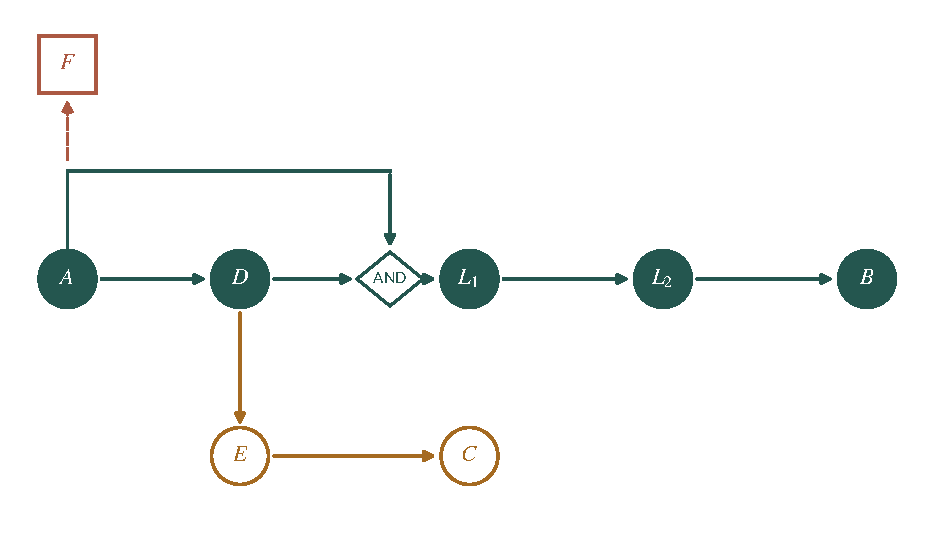
\includegraphics[width=\linewidth]{cover_field.pdf}
\vspace{4pt}
{\sffamily\fontsize{9}{12}\selectfont\color{KomorebiMuted}The proof is a certified core. The field retains the surrounding mathematics.\par}
\vfill
{\sffamily\bfseries\fontsize{11}{14}\selectfont\color{KomorebiInk}Komorebi P.\par}
\vspace{6pt}
{\sffamily\fontsize{9}{12}\selectfont\color{KomorebiMuted}Monograph edition 1.8.0\quad /\quad 19 October 2026\par}
\vspace*{3mm}
\end{titlepage}
\pagenumbering{roman}
\markboth{Monograph}{Monograph}
\section*{Preface}
\addcontentsline{toc}{section}{Preface}
A proof establishes an implication. The work surrounding that proof may answer other questions: why a definition was chosen, which hypothesis prevented an argument from failing, or how a change of representation opened a route that had not previously been visible. Publishing a certificate and preserving this larger mathematical record are related tasks, but they are not the same task.

Proof Path Theory studies that distinction through explicit finite objects. A proof field contains typed claims, justifications, evidence, and targets. Each justification requires all of its listed premises, while alternative justifications supply different routes to a conclusion. A certified derivation lies inside this field without converting its conjectures, examples, and unsuccessful attempts into additional proof steps.

The theory has two complementary directions. One selects or compresses a record while asking what remains recoverable. The other assembles local descriptions into coherent realizations. The first leads to certificate complexity, task sufficiency, information loss, and retention. The second gives a precise connection with Komorebi Space through local rule models, restriction maps, and gluing. A separate linear model yields positive realization certificates, negative obstruction witnesses, and exact observation counts.

Failed approaches remain part of the ambient record for a reason. They may isolate a missing hypothesis or reveal a limitation of one method. Their value does not turn a failed search into a proof of impossibility. A refutation must identify the assertion it refutes, the assumptions under which it applies, and the witness that establishes the failure. That scope is as important as the witness itself.

The later chapters examine how an archive changes and how its claims are evaluated. Their review and queue models are deliberately conditional. A covariance formula describes a specified dependence model, not an empirical diagnosis of a community. A record of social reception does not determine whether a proof is valid. Keeping those distinctions explicit allows the theory to study the transmission of mathematics without replacing mathematical standards with social judgments.

The mathematical ingredients come from proof theory, graph theory, category theory, linear algebra, information theory, and optimization. Their role here is to form one account of certified reasoning and the surrounding information that later inquiry may need. Familiar ingredients are not concealed, and a new notation is not presented as evidence of new mathematical truth.

This monograph preserves written proofs, finite examples, and the connection to the accompanying implementation. Its formal concordance identifies the selected Lean interfaces. The aim is a record that a reader can inspect at several levels: the statement, its argument, the hypotheses that make it valid, and the computational evidence supplied for its implementation.

\clearpage
\section*{Reading map}
\addcontentsline{toc}{section}{Reading map}
The five parts follow one mathematical record from discovery to certification, realization, compression, review, and reuse. The visual studies work through actual finite examples rather than replacing the proofs.

\begin{figure}[H]\centering
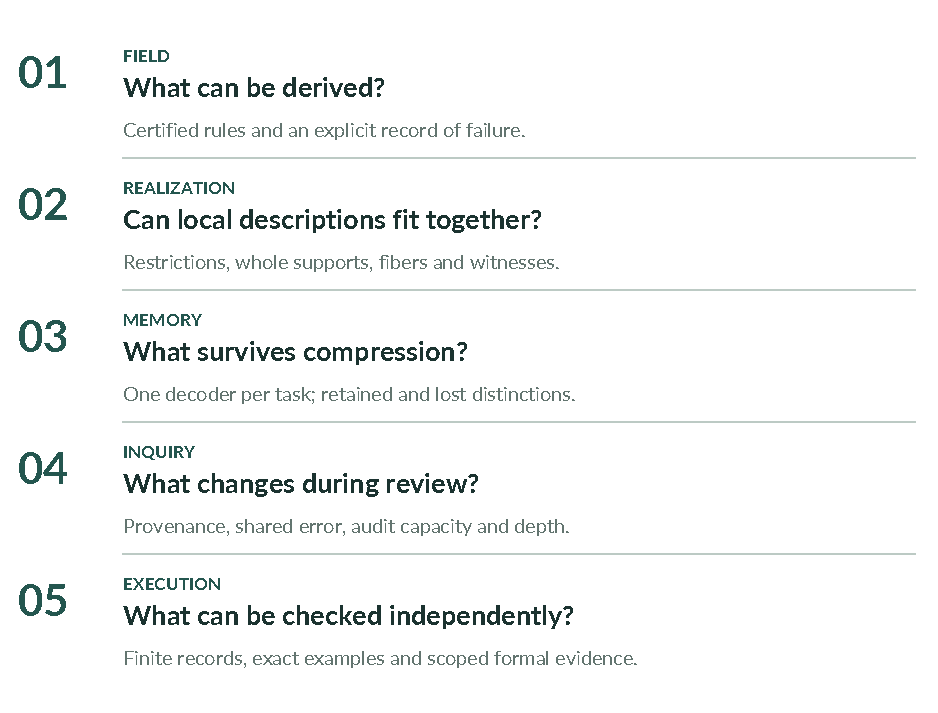
\includegraphics[width=\linewidth]{fig_00_theory_map.pdf}
\caption{Five questions organize the monograph. The order is a reading route, not a claim that one kind of evidence replaces another.}
\label{fig:theory-map}
\end{figure}

\begin{minipage}[t]{0.47\linewidth}
{\sffamily\bfseries\color{KomorebiTeal}A short technical route}\par\smallskip
Begin with Sections~\ref{sec:old3}, \ref{sec:old4}, \ref{sec:old24}, and \ref{sec:old7}. For collective interpretation, read Sections~\ref{sec:old17} and \ref{sec:old25} together.
\end{minipage}\hfill
\begin{minipage}[t]{0.47\linewidth}
{\sffamily\bfseries\color{KomorebiTeal}Evidence in this edition}\par\smallskip
The 41 prior result groups are retained. Six new groups specify trace checking and typed exchange. Eighteen Lean modules were freshly built, replayed with Lean's kernel, and axiom audited. Exact finite checks remain separate from the formal proofs.
\end{minipage}

\clearpage
\tableofcontents
\clearpage
\pagenumbering{arabic}
\monographpart{Proof fields and certificates}{Fields and certificates}{A completed proof occupies only part of its surrounding field. Keep the successful deduction, but do not confuse its unused alternatives with either errors in that deduction or proofs of impossibility.}

\section{Introduction}
\label{sec:old1}

A published proof often presents an argument after its exploratory work has been compressed. Definitions have stabilized, unsuccessful approaches have been set aside, and a long calculation may now appear as a lemma. The change of representation that first made the argument visible can disappear into a single sentence. Such compression is often useful: it leaves a certificate that is easier to check and reuse.

Compression can also remove mathematical information that is not needed for the present theorem. An example may explain why a definition was chosen. A failed route may isolate the exact boundary of a method. An alternative proof may carry a bridge to another field. A computation may reveal a stronger statement than the one originally sought. None of these objects is automatically part of the final implication
\[
A\vdash B.
\]
They may still be part of the mathematical event that produced it.

Proof Path Theory studies this larger object without changing the standard of proof. Its central separation is
\[
\boxed{
\text{certificate of validity}
\quad\ne\quad
\text{expanded discovery field}.
}
\]
The certificate answers whether the conclusion follows. The discovery field records how the conclusion became reachable, what alternatives were considered, what was lost during compression, and which omitted structures may matter later.

The construction begins with a typed field of claims, justifications, evidence, and targets. Its certified rules determine which targets are derivable. A certificate selects enough of those records to support a declared conclusion, while the ambient field can retain unresolved or refuted alternatives.

A second layer asks what survives when the field is compressed. The answer depends on the questions that a representation must support. An archive intended for future discovery may preserve examples and failed approaches that a verification certificate can omit. A bridge graph makes one such retention problem precise.

The final layer concerns the continuing life of the archive. Revisions change the set of claims that need review. Shared errors affect the information supplied by multiple reviewers. Audit capacity limits how quickly new candidates can be checked. These models are connected by their declared proof objects, without treating social judgments as substitutes for deduction.



\begin{figure}[htbp]
\centering
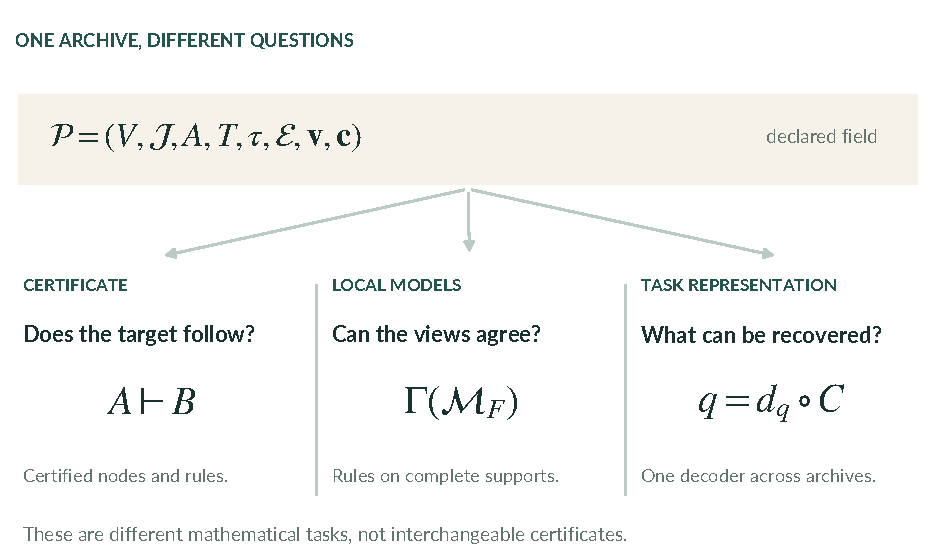
\includegraphics[width=\linewidth]{fig_01_architecture.pdf}
\caption{Three different questions about the same declared archive. A certificate records derivability, local models record rule compatibility, and a task representation records recoverable information. None of these questions subsumes the others without additional hypotheses.}
\label{fig:architecture}
\end{figure}

Komorebi Space enters when local descriptions of a proof field must agree. The construction of local rule models supplies actual restriction maps, not merely a visual analogy between two graphs. A gluing theorem identifies a sufficient condition for assembling those models, and a counterexample explains why pairwise dependency checks can miss a conjunctive rule. In a separate linear setting, the size of a realization fiber measures exactly what a new observation distinguishes.

The implemented proof fields are finite and acyclic. Some structural statements, including rule soundness and the linear separation alternative, are given in greater generality where their hypotheses allow it. Extensions to infinite search, probabilistic inference, and higher categorical proof objects require their own assumptions. Background on formal proof systems may be found in \cite{buss,troelstra}.


\section{Claim types and logical boundaries}
\label{sec:old2}

A useful theory of proof paths must not turn every recorded object into a proof step. A notebook may contain a theorem, a conjecture, a failed analogy, a numerical experiment, and a historical interpretation on the same page. Their coexistence does not give them the same logical status.

\begin{definition}[Evidence kind]
\label{res:2:1}
An evidence kind is a declared type attached to a record supporting a claim or justification. The core finite vocabulary used here is
\[
\begin{aligned}
&\text{formal proof},\quad \text{assumption},\quad \text{exact computation},\\
&\text{numerical evidence},\quad \text{conjecture},\quad \text{external result},\\
&\text{counterexample},\quad \text{interpretation}.
\end{aligned}
\]
An evidence record also states its source, scope, and whether it certifies the justification to which it is attached.
\end{definition}

The word ``certifies'' is deliberately separate from the evidence label. An exact computation may certify a finite identity while providing only numerical evidence for a general statement. An external result may certify a step only on the domain covered by its hypotheses. The scope field is therefore part of the mathematical object.

\begin{warning}[Evidence types are not one ranking]
\label{res:2:2}
The evidence kinds do not form a universal total order. A formal proof of a weak statement and an exact computation of a stronger finite instance cannot be compared by one scalar without specifying the task. The ledger retains type and scope instead of replacing them with a single confidence number.
\end{warning}

This separation will be used throughout. Candidate edges may remain in the discovery field, but only certified edges enter a proof certificate.


\section{Typed proof fields}
\label{sec:old3}

The first formal object is a directed hypergraph. A justification may require several premises at once, and a claim may admit several alternative justifications.

\begin{definition}[Typed proof field]
\label{res:3:1}
A finite typed proof field is a tuple
\[
\Pcal=(V,\Jcal,A,T,\tau,\Ecal,\mathbf v,\mathbf c),
\]
where:
\begin{itemize}
\item $V$ is a finite set of claim nodes.
\item $\Jcal$ is a finite set of justifications.
\item Each $j\in\Jcal$ has a finite premise set $\operatorname{prem}(j)\subseteq V$ and one conclusion $\operatorname{con}(j)\in V$.
\item $A\subseteq V$ is the set of required premises of the declared judgment.
\item $T\subseteq V$ is the nonempty target set.
\item $\tau$ assigns node and justification types.
\item $\Ecal$ is a typed evidence ledger.
\item $\mathbf v$ assigns nonnegative value coordinates to nodes.
\item $\mathbf c$ assigns nonnegative storage, audit, recovery, and cognitive costs.
\end{itemize}
The dependency graph contains an edge $u\to v$ whenever $u\in\operatorname{prem}(j)$ and $v=\operatorname{con}(j)$ for some justification $j$. It is required to be acyclic.
\end{definition}

A single justification is conjunctive in its premise set. All listed premises must be available. Multiple justifications with the same conclusion are alternatives. This gives the familiar AND/OR structure of proof search without forcing it into an ordinary graph.

\begin{definition}[Admissible leaf]
\label{res:3:2}
A node is an admissible leaf when it is a required premise, a declared axiom, or an explicitly admitted external result. Write $L$ for this set, so $A\subseteq L$. A certified justification with no premises can also derive a node, but it remains a justification and need not make that node a member of $L$. The distinction matters when extracting the smallest certificate.
\end{definition}

Required premises are not necessarily the entire assumption context. Admitted axioms and external results remain visible in the supporting ledger. The notation $A\vdash B$ is relative to that declared background and does not erase those dependencies. A comparison between certificates must retain the assumptions under which each certificate is valid.

\begin{definition}[Certified subfield]
\label{res:3:3}
The certified subfield $\Pcal^{\mathrm{cert}}$ contains every node of $\Pcal$ and only those justifications accepted by the declared certification policy. Evidence and scope are part of that policy. A certification flag records acceptance: it is not itself a proof that the rule is sound under an intended mathematical interpretation. That separate soundness contract is made explicit in Section~\ref{sec:old24}.
\end{definition}

\begin{definition}[Derivability]
\label{res:3:4}
Let $K\subseteq V$ be a selected node set and let $H\subseteq\Jcal$ be a selected justification set. The derivable set $D(K,H)$ is the least subset of $K$ satisfying:
\begin{enumerate}[label=\textup{(\roman*)}]
\item every selected admissible leaf belongs to $D(K,H)$.
\item if $j\in H$, $\operatorname{prem}(j)\subseteq D(K,H)$, and $\operatorname{con}(j)\in K$, then $\operatorname{con}(j)\in D(K,H)$.
\end{enumerate}
When only certified justifications are allowed, write $D_{\mathrm{cert}}(K,H)$.
\end{definition}

\begin{proposition}[Finite derivability]
\label{res:3:5}
For a finite acyclic proof field, $D(K,H)$ is uniquely determined and can be computed in one topological pass through the dependency graph.
\end{proposition}

\begin{proof}
Acyclicity gives a topological ordering of the nodes. Begin with the selected admissible leaves. At each later node, test whether one selected incoming justification has all of its premises already derived. Add the node exactly when such a justification exists. No later step can change the status of an earlier node because all dependencies point forward. The resulting set satisfies the closure rules. Any set satisfying the rules must contain every node added by this pass, so the result is the least such set and is unique.
\end{proof}

\begin{figure}[htbp]
\centering
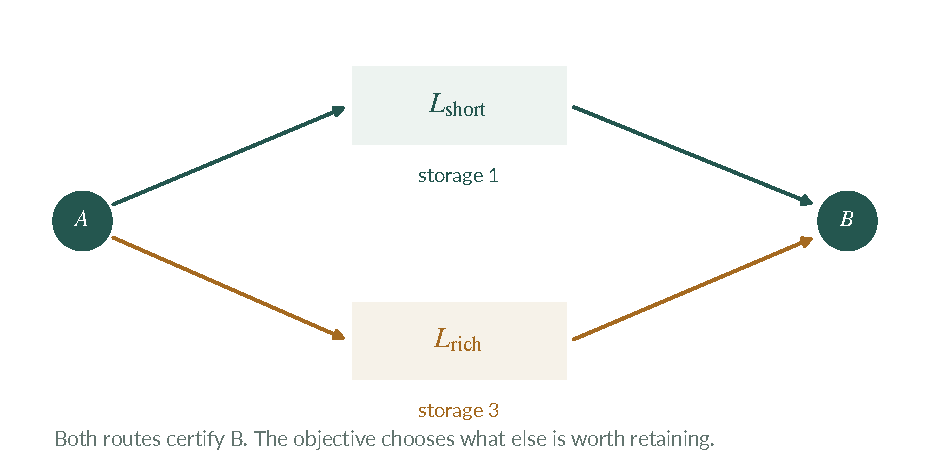
\includegraphics[width=\linewidth]{fig_03_alternative_hypergraph.pdf}
\caption{Two certified routes in \protect\path{alternative_proofs.json}. Their stored node costs are one and three. A storage objective selects the short route, while a task requiring explanatory information can prefer the richer route. Alternative derivations are OR choices, not extra conjunctive premises.}
\label{fig:andor}
\end{figure}


\section{The ambient proof field and the meaning of failure}
\label{sec:old22}
\label{sec:ambient}

A finished proof is rarely the only route the researcher could have explored. An archive often contains sketches that were never completed, arguments that failed because of a specific hypothesis, conjectured bridges that remain untested, and genuinely refuted local constructions. It is tempting to call this whole archive a proof, but doing so would erase the distinction between a certified result and a record of exploration. The \emph{ambient proof field} provides a more precise language: it is the declared field of reachable or recorded mathematical states and typed candidate transitions in which certified proof paths form a distinguished subfield.

The finite hypergraph model permits \path{failed_route}, \path{boundary_case}, and \path{counterexample} nodes. Their presence is useful, but none is a logically justified global nonexistence claim by itself. A failed search is not necessarily a proof of impossibility. A counterexample to one proposed lemma is not necessarily a counterexample to the goal. An exact obstruction must have a declared scope and a checkable witness.

\begin{definition}[Scoped branch assessment]
\label{res:22:1}
Let $\Pcal$ be a finite typed proof field with declared premises $A$ and target $t$. An exploratory branch is a finite sequence of candidate justifications whose certification and outstanding obligations are explicitly recorded. Its assessment is one of the following, relative to stated premises and rules:
\begin{enumerate}[label=\textup{(\roman*)}]
\item \emph{Open}: obligations remain unresolved.
\item \emph{Abandoned}: exploration stopped without a certificate of impossibility.
\item \emph{Locally refuted}: a checked counterexample or obstruction excludes a stated intermediate step under specified hypotheses.
\item \emph{Certified}: the selected justifications meet the declared proof certificate conditions.
\end{enumerate}
An assessment is a record of the branch, not a truth value assigned to every possible proof of $t$.
\end{definition}

\begin{proposition}[Local failure does not imply global failure]
\label{res:22:2}
A finite proof field may contain a locally refuted branch to target $t$ while also containing a certified derivation of $t$ from its declared premises.
\end{proposition}
\begin{proof}
Take a premise $A$ and two alternative candidate derivations of $t$. Let the first use a proposed intermediate lemma $L$ that has a checked counterexample, so the corresponding justification is not certified. Let the second use a distinct certified justification from $A$ to $t$. The certified closure reaches $t$ by the second route. The failed first route remains a valid record of unsuccessful exploration, but cannot negate the existence of the second certificate. The same example can be represented by the alternative justification hypergraph developed earlier.
\end{proof}



The logical lesson is substantive for machine reasoning. A search timeout, budget exhaustion, invalid intermediate conjecture, or failure to find a proof all have different meanings. Only a certificate whose conclusion explicitly concerns nonexistence under a declared model and scope licenses a nonexistence claim. This is especially important when a failed branch is used to prune an automated search. Pruning the refuted step may be safe, while pruning its entire goal may discard a genuine proof.

\begin{proposition}[Scoped refutation survives unchanged context]
\label{res:22:3}
Suppose a witness $w$ is verified by a sound checker to refute the predicate $L$ under assumptions $A$. In any later archive revision that retains the same interpretation of $L$, the same assumptions, and the checker's verification rules, $w$ remains a refutation of $L$. No conclusion follows about different predicates, altered assumptions, or alternative branches to a different goal.
\end{proposition}
\begin{proof}
The verification of $w$ depends only on the declared predicate, assumptions, and checking rules. An append-only collection of unrelated exploratory records does not alter those inputs. Therefore the same verification remains valid. When any of those inputs changes, the earlier check no longer certifies the revised claim without an explicit comparison theorem.
\end{proof}

This is a qualified stability principle, not a general theorem that proof search is decidable. The append-only derivability result of Section~\ref{sec:versioned} concerns certified edges. The present proposition concerns the narrower persistence of a checked counterexample under a fixed interpretation. Both retain scope as part of the mathematical data.


\section{Certificates and verification closure}
\label{sec:old4}

\begin{definition}[Certificate]
\label{res:4:1}
A certificate for a nonempty requested target set $T_0\subseteq V$ is a pair
\[
\Ccal=(K,H),
\qquad K\subseteq V,
\qquad H\subseteq\Jcal^{\mathrm{cert}},
\]
such that
\[
A\cup T_0\subseteq K
\qquad\text{and}\qquad
T_0\subseteq D_{\mathrm{cert}}(K,H).
\]
Order certificates componentwise: $(K,H)\leq(K^{\prime},H^{\prime})$ means $K\subseteq K^{\prime}$ and $H\subseteq H^{\prime}$. A least certificate is contained in every certificate for the same request. Minimizing only the node set, only the justification set, or a numerical cost is a different objective.
\end{definition}

The usual target request is a subset of $T$, but an intermediate node may be requested for local analysis. Only a justification whose premises have been derived and whose conclusion is selected can contribute to the derivation. A record may retain other, inactive justifications without using them as proof steps. Extra records cannot lower a nonnegative additive cost, although zero costs can allow several minimizing records.

\subsection{The fixed AND-DAG case}

The simplest case occurs when each relevant node that is not an admissible leaf has one certified incoming justification. Backward expansion stops at admissible leaves. A proof of a statement that has already been admitted as a leaf is not required to use that statement.

\begin{definition}[AND-DAG]
\label{res:4:2}
Starting at $T_0$, expand backward only at nodes outside $L$. The field is an AND-DAG relative to $T_0$ when every node reached outside $L$ has exactly one certified incoming justification. Every premise of that justification is then expanded in the same manner. The process may terminate at an admissible leaf or at a certified justification with no premises.
\end{definition}

Let $\Anc_L(T_0)$ denote the premise nodes reached by this backward expansion, stopping at $L$. Let $H_{\mathrm{core}}$ contain exactly the justifications selected at expanded nodes outside $L$.

\begin{theorem}[Unique verification core]
\label{res:4:3}
\label{thm:and-core}
Let $\Pcal$ be a finite acyclic AND-DAG relative to $T_0$. Put
\[
K_{\mathrm{core}}=A\cup T_0\cup\Anc_L(T_0).
\]
Then $(K_{\mathrm{core}},H_{\mathrm{core}})$ is a certificate and is the least certificate under componentwise inclusion. In particular it is the unique inclusion-minimal certificate pair for this recorded inference problem.
\end{theorem}

\begin{proof}
Backward expansion terminates because the dependency graph is finite and acyclic. Every terminal node is either an admissible leaf or the conclusion of the selected justification with no premises. A forward topological pass therefore derives every expanded node. The required premises in $A$ are admissible and are retained even if the target does not use them. Thus the constructed pair is a certificate.

Now let $(K,H)$ be any certificate for the same request. It contains $A\cup T_0$. If a requested or required predecessor node is outside $L$, its derivation must use its unique certified incoming justification. That justification belongs to $H$, and every one of its premises belongs to $K$. Repeating the argument forces all of $\Anc_L(T_0)$ and $H_{\mathrm{core}}$. At nodes in $L$ the argument stops. Hence $K_{\mathrm{core}}\subseteq K$ and $H_{\mathrm{core}}\subseteq H$, which proves the least-pair assertion.

Minimizing one coordinate alone does not make the whole record unique. One may add an irrelevant node without changing the least justification set, or retain an unused rule without changing the least node set. The componentwise statement avoids this ambiguity.
\end{proof}

\begin{corollary}[Linear extraction]
\label{res:4:4}
With indexed certified adjacency and constant-time membership bookkeeping, the core can be extracted in time linear in $|A|$ plus the number of visited nodes, selected justifications, and premise incidences.
\end{corollary}

This bound concerns the indexed graph algorithm. It is not a verified running-time bound for every scanning routine in the reference Python package.

\begin{figure}[htbp]
\centering
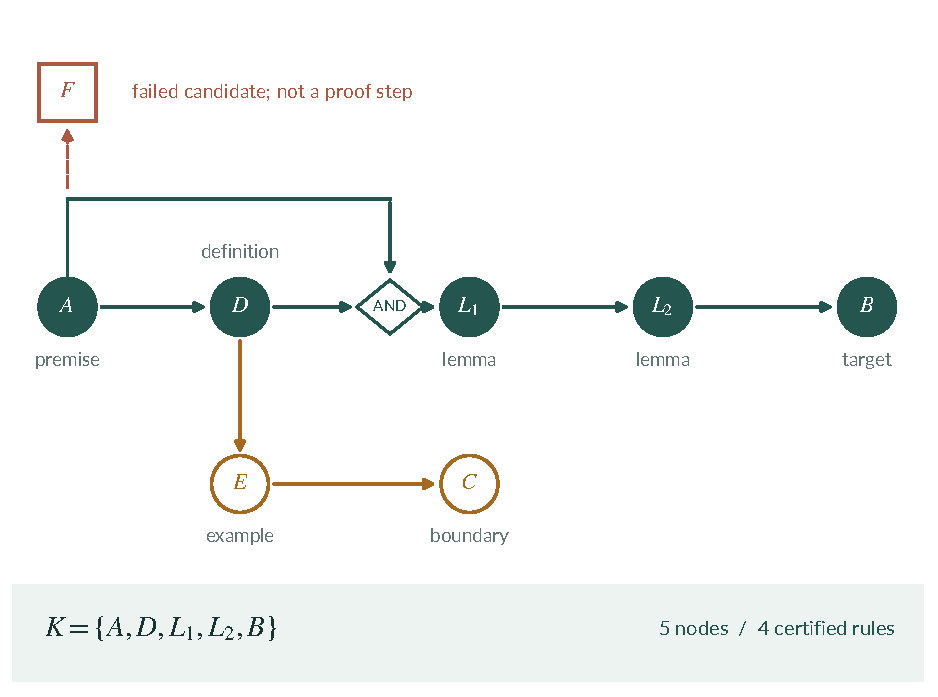
\includegraphics[width=\linewidth]{fig_02_and_dag_core.pdf}
\caption{The canonical \protect\path{and_dag.json} example. The AND gate requires both $A$ and $D$ for $L_1$. Its least certificate contains five nodes and four certified rules. The gold branch is certified but unnecessary for $B$. The dashed route to $F$ is uncertified and cannot enter the certificate.}
\label{fig:andcore}
\end{figure}

\begin{remark}
\label{res:4:5}
The theorem identifies the minimum certificate for the recorded derivation. It does not claim that the derivation is globally shortest among all possible proofs of the theorem. A different proof field may have a smaller core.
\end{remark}


\section{Alternative derivations and certificate complexity}
\label{sec:old5}

When a claim admits several certified justifications, certificate extraction is no longer a backward closure problem. A local choice may be reused by several later obligations, which couples decisions across the field.

\begin{problem}[Minimum Certificate Decision]
\label{res:5:1}
Given a finite acyclic certified proof field, a target set, nonnegative integer node and justification costs, and a budget $B$, determine whether a certificate of total cost at most $B$ exists.
\end{problem}

\begin{theorem}[Minimum certificate selection is NP-complete]
\label{res:5:2}
\label{thm:minimum-certificate}
Minimum Certificate Decision is NP-complete, even when every nonzero cost is a unit node cost and all justification costs are zero.
\end{theorem}

\begin{proof}
The problem belongs to NP. A proposed node and justification set can be checked in polynomial time by verifying references, computing derivability in topological order, and summing costs.

For NP-hardness, reduce Set Cover. Let $U=\{u_1,\ldots,u_m\}$ be the universe, let $S_1,\ldots,S_n\subseteq U$ be the available sets, and let $k$ be the cover budget. Construct one optional admissible leaf node $s_i$ for each set $S_i$, with unit cost. Construct one zero-cost obligation node $e_j$ for each element $u_j$. Whenever $u_j\in S_i$, add a certified justification
\[
\{s_i\}\Longrightarrow e_j.
\]
Add a zero-cost target node $t$ with the certified justification
\[
\{e_1,\ldots,e_m\}\Longrightarrow t.
\]
The dependency graph is acyclic. A certificate for $t$ must derive every $e_j$. Deriving $e_j$ requires at least one selected source node $s_i$ with $u_j\in S_i$. One selected $s_i$ may discharge several obligations, and its cost is paid once. Therefore a certificate of cost at most $k$ exists exactly when the original Set Cover instance has a cover of size at most $k$. The reduction is polynomial.
\end{proof}

\begin{figure}[htbp]
\centering
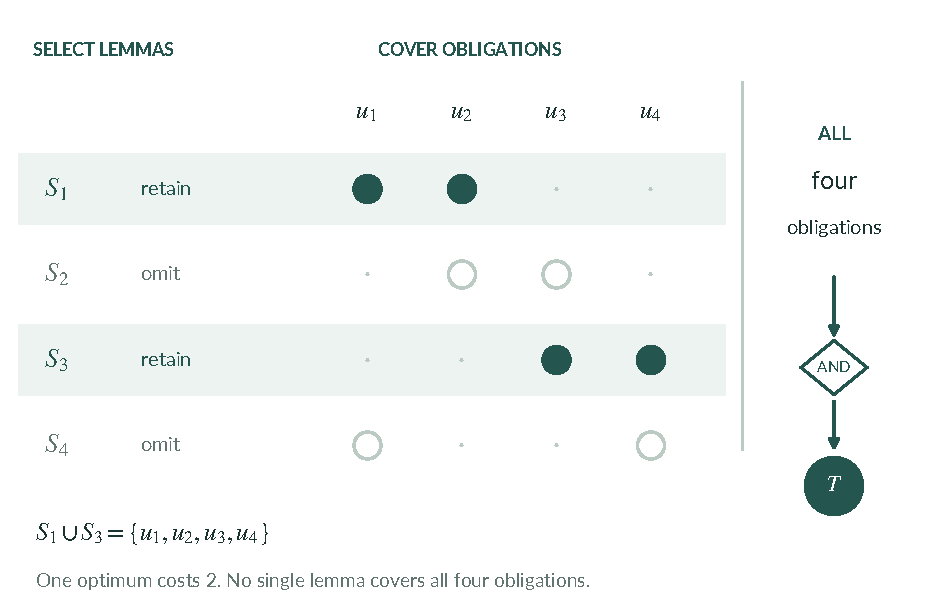
\includegraphics[width=\linewidth]{fig_04_certificate_complexity.pdf}
\caption{The Set Cover example as a membership matrix. Filled marks belong to the selected rows $S_1$ and $S_3$; open marks show unselected memberships. Every obligation is covered. The target requires all four obligations through one AND rule. The exact minimum is two, although the minimizing pair need not be unique.}
\label{fig:setcover}
\end{figure}

\begin{remark}[Algorithmic consequence]
\label{res:5:3}
Exhaustive certificate selection is useful for small fields or fields with few alternatives. The reference implementation uses branch and bound with an explicit search-state limit. Its result is optimal for the stored finite cost data when the search completes. It does not remove the exponential worst case. The decision theorem concerns integer costs, while the Python interface accepts finite floating-point costs and compares their exact stored binary values as rationals. Printed cost totals remain floating-point summaries. The input conversion does not recover an intended real or decimal value that was never represented. See \cite{garey-johnson} for the background complexity language.
\end{remark}


\section{Certified paths as a category}
\label{sec:old6}

The hypergraph model records local justifications. A complementary construction treats complete certified transformations as morphisms. It uses the usual category of paths \cite{maclane}.

\begin{definition}[Certified proof category]
\label{res:6:1}
Fix a directed graph of typed mathematical states and certified primitive transformations. Its path category $\mathsf{Cert}$ has these states as objects and finite composable paths as morphisms. The empty path is an identity, and composition is concatenation. One may further identify paths by a declared congruence compatible with concatenation. Associativity and the identity laws then hold by construction.
\end{definition}

A state may be a proposition, a diagram, an exact finite computation, a coordinate representation, or a structured collection of claims. Candidate analogies may live in a larger discovery graph, but they do not enter $\mathsf{Cert}$ until their logical force and domain have been certified.

\begin{proposition}[Functorial transport]
\label{res:6:2}
Let $F:\mathsf{Cert}_1\to\mathsf{Cert}_2$ be a functor. If
\[
A\xrightarrow{f_1}S_1\xrightarrow{f_2}\cdots\xrightarrow{f_r}B
\]
is a certified path in $\mathsf{Cert}_1$, then
\[
F(A)\xrightarrow{F(f_1)}F(S_1)\xrightarrow{F(f_2)}\cdots\xrightarrow{F(f_r)}F(B)
\]
is a certified path in $\mathsf{Cert}_2$.
\end{proposition}

\begin{proof}
A functor maps objects to objects and morphisms to morphisms. It preserves identities and composition. The image of the composite path is therefore the composite of the image morphisms, which is certified in the target category.
\end{proof}

The proposition transports certification inside the two declared categories. To interpret that transport as preservation of a mathematical judgment, the target category and functor must also have sound interpretations of their objects and rules. These requirements cannot be inferred merely from the word functor. Under that contract, different representations can preserve a judgment while exposing different features of its argument. The category language is standard \cite{maclane}.

\begin{definition}[Compositional certificate map]
\label{res:6:3}
A compositional certificate map is a functor
\[
\Ccal:\mathsf{Expanded}\longrightarrow\mathsf{Certificate}
\]
that sends expanded certified paths to checkable certificate paths and preserves identity and composition.
\end{definition}

\begin{proposition}[Local audit composes]
\label{res:6:4}
If every primitive morphism in a finite path has an auditable certificate and the certificate map is compositional, then the composite path is auditable from the primitive certificates and the declared composition rules.
\end{proposition}

\begin{proof}
Proceed by induction on path length. The length-zero case is an identity. Assume the first $r$ morphisms have an auditable composite certificate and append one certified morphism. Functoriality identifies the new certificate with the composition of the earlier certificate and the primitive certificate of the appended morphism. The declared composition rule completes the audit.
\end{proof}


\monographpart{Coherent realization and information}{Coherent realization}{Compatibility, extension, obstruction, and ambiguity become concrete once the views and protected observations are specified. This part gives the actual bridge to Komorebi Space.}

\section{Komorebi Space, realization fibers, and informative questions}
\label{sec:old23}
\label{sec:komorebi-bridge}

Komorebi Space supplies a natural setting for studying the proof field's coherent realizations. Here the connection is \emph{relative} to an explicitly chosen system of views. Nothing in a finite proof hypergraph canonically supplies one universal category of all proofs, and a formal proof term is not automatically equivalent to an intended semantic object. The view system must be stated, together with its restrictions and the observations that are required to survive.

\begin{definition}[Coherent views of a proof field]
\label{res:23:1}
Choose a finite collection of views $V$, fibers $F_v$ of local proof states or annotations, and for each declared directed edge $e:v\to w$ a restriction map $e^*:F_w\to F_v$. The \emph{strict realization set} is
\[
\Gamma(F)=\big\{(x_v)\in\prod_{v\in V}F_v : e^*(x_w)=x_v\text{ for every declared edge }e\big\}.
\]
The \emph{extension fiber} of prescribed information $s$ on $U\subseteq V$ consists of those global coherent families whose restrictions equal $s$. If the edges form a category, the usual functorial composition equations are additional explicit obligations.
\end{definition}

The finite implementation \path{ambient.py} realizes this edge-defined model exactly. The gluing condition should not be weakened to covering the objects alone: a compatibility equation is attached to an edge and must appear in at least one patch.

\begin{theorem}[Finite arrow-cover gluing]
\label{res:23:2}
Suppose patches $U_i\subseteq V$ cover every view and every declared edge has both endpoints in some $U_i$. Let $s_i$ be coherent assignments on $U_i$ that agree on all overlaps. There is a unique global coherent assignment $s\in\Gamma(F)$ restricting to every $s_i$.
\end{theorem}
\begin{proof}
For each view $v$, choose any patch containing it and define $s(v)$ to be the value supplied by that patch. Agreement on overlaps makes this independent of the choice. For a declared edge $e:v\to w$, choose a patch containing both endpoints. The local assignment on that patch obeys $e^*s(w)=s(v)$, so the global assignment is coherent. It is the only possible glue because every coordinate was prescribed by at least one patch.
\end{proof}

\begin{example}[Object coverage cannot replace arrow coverage]
\label{res:23:3}
Let $V=\{v,w\}$ with an edge $v\to w$, both fibers $\{0,1\}$, and identity restriction. Singleton patches prescribe $s(v)=0$ and $s(w)=1$. These assignments cover all views and agree on their empty overlap. There is no global coherent assignment with those coordinates. The missing ingredient is the edge condition, not the availability of the two individual values.
\end{example}

The theorem is a finite instance of the strict gluing construction in \emph{Komorebi Space} \cite{komorebi-space}. It does not claim a general stack theorem for nonabelian proof objects. Gluing up to isomorphism requires the identifications and their coherence witnesses, which are retained in the corresponding groupoid setting.

\subsection{Exact finite realization and obstruction certificates}

A second connection is quantitative. Work over $\mathbb F_2$ with $E=\mathbb F_2^n$. Let $A:E\to\mathbb F_2^m$ impose coherence, $P:E\to\mathbb F_2^p$ retain prescribed information, and $x\in E$ be a raw candidate. Define
\[
\mathfrak K_P(x)=\{y\in E:Ay=0,\ Py=Px\},\qquad
M=\begin{bmatrix}A\\P\end{bmatrix},\quad
b=\begin{bmatrix}0\\Px\end{bmatrix}.
\]
This is a finite linear realization fiber. The equation $My=b$ does not by itself produce a solution. Compatibility of the prescribed information must first be established.

\begin{theorem}[Finite realization alternative and ambiguity]
\label{res:23:4}
Exactly one of the following holds:
\begin{enumerate}[label=\textup{(\roman*)}]
\item $My=b$ has a solution $y_0$. Its complete solution set is $y_0+H$, where $H=\ker A\cap\ker P$, and
\[
|\mathfrak K_P(x)|=2^{n-\operatorname{rank}(M)}.
\]
\item A row vector $\lambda$ exists with $\lambda M=0$ and $\lambda b=1$. It is a directly checkable certificate that $\mathfrak K_P(x)=\varnothing$.
\end{enumerate}
\end{theorem}
\begin{proof}
If $My_0=b$, any other solution differs from $y_0$ by an element of $\ker M=H$, and every such difference gives another solution. Rank nullity gives $\dim H=n-\operatorname{rank}(M)$. If $b$ is not in the column space of $M$, linear algebra supplies a linear functional that vanishes on that column space and takes value $1$ on $b$. Expressing it as a row vector gives $\lambda$. Conversely such a witness contradicts any proposed equation $My=b$, since it would imply $0=\lambda My=\lambda b=1$. These cases are mutually exclusive and exhaustive over a field.
\end{proof}

This negative certificate is a concrete instance of the protected obstruction principle from Komorebi Space. Its scope is exactly the finite linear system $My=b$. It is not a certificate that some broad mathematical conjecture is unprovable.

\subsection{The information gained by a new observation}

Suppose the realization fiber is nonempty and a new linear observation $Q:E\to\mathbb F_2^q$ becomes available. The right question is not how many bits appear in the output of $Q$ but how many remaining degrees of freedom in the fiber it distinguishes.

\begin{theorem}[Exact observation gain]
\label{res:23:5}
Give the nonempty finite affine fiber $y_0+H$ the uniform distribution. Then the Shannon entropy of the observed value $Qy$ is
\[
H(Qy)=\operatorname{rank}(Q|_H)\quad\text{bits}.
\]
For every observation value that actually occurs, the corresponding conditional fiber contains
\[
2^{\dim H-\operatorname{rank}(Q|_H)}
\]
realizations. Thus the uncertainty reduction is exactly $\operatorname{rank}(Q|_H)$ bits.
\end{theorem}
\begin{proof}
The image $Q(H)$ is a vector subspace of dimension $r=\operatorname{rank}(Q|_H)$, so the observed values form the affine set $Qy_0+Q(H)$ of size $2^r$. Every such value has a preimage that is a coset of $H\cap\ker Q$, whose dimension is $\dim H-r$ by rank nullity. Equal fiber cardinalities make the induced output distribution uniform on $2^r$ values. Its entropy is $\log_2(2^r)=r$, and each conditional fiber has cardinality $2^{\dim H-r}$.
\end{proof}

\begin{example}[One informative question]
\label{res:23:6}
Let $y=(a,b,c)\in\mathbb F_2^3$ with $a+b+c=0$ and protected value $a=0$. The realization fiber is $\{(0,0,0),(0,1,1)\}$. It has one bit of ambiguity. Observing $b$ resolves that bit exactly. Observing $a$ supplies no new information, despite being a perfectly valid measurement. This difference is measured by the rank of the observation restricted to $H$, rather than by the output width of the observation.
\end{example}

The module \path{realization.py} computes these quantities through exact binary row reduction, and returns an explicit linear witness when the protected realization is impossible. The program does not enumerate all solutions, although the tests compare its results with exhaustive enumeration on small cases. The entropy statement uses Shannon entropy \cite{cover-thomas} and assumes uniform sampling of the compatible realizations. It does not assert a universal prior over mathematical discoveries, or that the most informative observation is automatically the most valuable research question once costs and task priorities are included.


\section{A checked realization bridge for proof fields}
\label{sec:old24}
\label{sec:checked-bridge}

The ambient interpretation can be made into a mathematical construction rather than left as an analogy. The important step is to specify what a local realization means. A node label may describe an arbitrary mathematical sentence, but a Boolean value attached to that node does not automatically evaluate that sentence. In this section it records membership in a set closed under the declared certified rules. This restricted interpretation has an exact soundness and completeness theorem. An interpretation in actual mathematical propositions is a separate contract.

\subsection{The declared rule system and its models}

Fix a node set $V$, a set $L\subseteq V$ of admissible leaves, and a set $J$ of justifications. A justification $j$ has a premise set $A_j$, a conclusion $c_j$, and a certification predicate. Define its support by
\[
S_j=A_j\cup\{c_j\}.
\]
A set $X\subseteq V$ is a \emph{model of the declared field} when $L\subseteq X$ and, for every certified $j$,
\[
A_j\subseteq X\quad\Longrightarrow\quad c_j\in X.
\]
Each justification is one implication with conjunctive premises. Alternative justifications remain separate implications. Uncertified attempts and failed-route annotations do not contribute a deduction rule merely by appearing in the archive.

Let $\operatorname{Der}_F$ be the inductively generated set obtained from the leaves by certified rules. For a finite field, repeated forward closure computes this set. It is not necessary to enumerate all valuations to perform that computation.

Every declared field of this positive-implication form has a model: the full set $V$. It contains every leaf and every rule conclusion. Nonexistence in the following extension problems therefore concerns prescribed local values or additional preservation requirements, not this unrestricted model space. This does not make every node derivable. Derivability is membership in the least model, not membership in some model.

\begin{theorem}[Soundness and relative completeness]
\label{res:24:1}
\label{thm:relative-completeness}
For every node $v$,
\[
v\in\operatorname{Der}_F
\quad\Longleftrightarrow\quad
\text{$v\in X$ for every model $X$ of the declared field}.
\]
If $v$ is not derivable, $\operatorname{Der}_F$ itself is a model omitting $v$.
\end{theorem}
\begin{proof}
Every model contains the leaves. Induction on a derivation shows that it contains the conclusion of every certified application whose premises have already been derived. Thus every model contains $\operatorname{Der}_F$. Conversely, the inductive constructors show that $\operatorname{Der}_F$ contains the leaves and is closed under every certified rule. It is therefore a model. Applying the universal condition to this particular model proves the reverse implication, and the same model gives the stated countermodel.
\end{proof}

This is relative completeness for the declared rule system, not completeness of arbitrary mathematical proof search. A missing theorem may simply require a rule or a lemma absent from the field. A failed search can therefore produce a useful countermodel to a proposed finite inference architecture without disproving the mathematical target.

For an intended interpretation $\mu:V\to\mathrm{Prop}$, the transfer to mathematical truth has explicit hypotheses: every leaf must satisfy $\mu$, and every certified rule must preserve $\mu$ from all its premises to its conclusion. Under those hypotheses, induction gives $v\in\operatorname{Der}_F\Rightarrow\mu(v)$. Lean checks this statement as \path{ProofPath.Field.semantic_soundness}. It does not infer those hypotheses from a JSON certification flag.

\subsection{From patches to a contravariant view system}

For a patch $U\subseteq V$, let $\mathcal M_F(U)$ consist of subsets $X_U\subseteq U$ which contain $L\cap U$ and obey every certified rule whose entire support lies in $U$. If $U\subseteq W$, define
\[
\rho_{U,W}:\mathcal M_F(W)\longrightarrow\mathcal M_F(U),
\qquad \rho_{U,W}(X_W)=X_W\cap U.
\]
This map is well defined. A rule supported in $U$ is also supported in $W$, and its conclusion remains in $U$. The restriction therefore preserves both the local leaves and the local implication conditions.

\begin{proposition}[The proof-field view laws]
\label{res:24:2}
The restriction maps satisfy
\[
\rho_{U,U}=\mathrm{id},\qquad
\rho_{U,W}\rho_{W,Z}=\rho_{U,Z}\quad(U\subseteq W\subseteq Z).
\]
Consequently $U\mapsto\mathcal M_F(U)$ is a contravariant set-valued view system on the inclusion order of patches.
\end{proposition}
\begin{proof}
Both laws are the corresponding intersection identities. For the second, $(X\cap W)\cap U=X\cap U$ because $U\subseteq W$. The values outside a patch are absent, or equivalently normalized to false in the Lean representation. There are no additional hidden coordinates.
\end{proof}

The strict Komorebi realization is now an actual set of coherent local models,
\[
\Gamma(\mathcal M_F)=
\left\{(X_U)_U:\rho_{U,W}(X_W)=X_U\text{ whenever }U\subseteq W\right\}.
\]
There is an explicit bijection
\[
\operatorname{Models}(F)\simeq\Gamma(\mathcal M_F),
\qquad X\longmapsto(X\cap U)_U.
\]
Its inverse evaluates a coherent family at the full patch $V$. Coherence shows that every other component is precisely the restriction of that value. The Lean declaration \path{ProofPath.Field.modelEquivSections} constructs this equivalence, using \path{ViewDiagram} and the actual local restriction maps.

The full-patch equivalence identifies the ambient construction. It does not prove that arbitrary prescribed proper-patch data extend: the full patch already contains the global problem. Extension from smaller views is the distinct content of the following theorem.


\studyhead{01}{The bridge is a restriction map}
For one certified rule $\{a,b\}\to c$ and no admissible leaves ($L=\varnothing$), there are seven global Boolean rule models. Only $(1,1,0)$ violates the implication. On either two-node patch below, the complete support is absent, so all four local valuations are admissible.

\begin{figure}[H]\centering
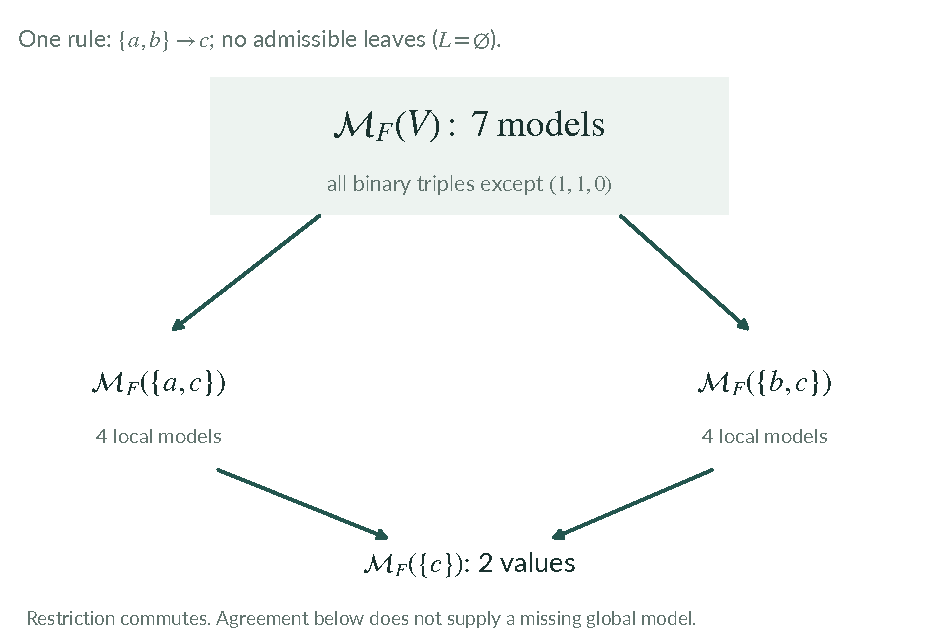
\includegraphics[width=\linewidth]{fig_16_restriction_bridge.pdf}
\caption{The local model sets and their actual restrictions. Each arrow is $\rho_{U,W}(X)=X\cap U$. The two ways of restricting a global model to $\{c\}$ agree. The diagram is counted directly from the finite rule model, with seven global models, four models on each two-node patch, and two overlap values.}
\label{fig:restriction-models}
\end{figure}

{\sffamily\bfseries\color{KomorebiTeal}What the diagram establishes}\par\smallskip
It displays the contravariant view construction and the consistency of restriction. The full-patch equivalence identifies global rule models with their coherent families of restrictions.

\medskip
{\sffamily\bfseries\color{KomorebiGold}What the diagram does not establish}\par\smallskip
A pair of matching proper-patch models need not be in the image of a global model. That extension question is controlled by the support of the rule, as the next study shows.
\clearpage

\subsection{The correct coverage condition is a whole support}

Let $(U_i)_{i\in I}$ cover the nodes. A family $X_i\in\mathcal M_F(U_i)$ is matching when
\[
X_i\cap U_j=X_j\cap U_i\qquad\text{for every }i,j.
\]
This equality includes agreement about false values, not merely common true values.

\begin{theorem}[Whole-support gluing]
\label{res:24:3}
\label{thm:support-gluing}
Suppose every certified justification has its whole support in some patch:
\[
\forall j\text{ certified},\quad\exists i\quad S_j\subseteq U_i.
\]
Then every matching family $(X_i)$ has a unique global field model $X$ satisfying $X\cap U_i=X_i$ for all $i$.
\end{theorem}
\begin{proof}
Set $X=\bigcup_iX_i$. Matching and node coverage imply $X\cap U_i=X_i$. A leaf belongs to some patch and hence to its local model, so $L\subseteq X$. Consider a certified rule whose premises belong to $X$. Choose a patch containing its entire support. Matching implies that every premise is true in that patch's local model, whose rule condition forces the conclusion. Hence $X$ obeys all certified rules. Any other global model with the specified restrictions agrees with $X$ at every node because the patches cover the nodes. This proves uniqueness.
\end{proof}

\begin{example}[Pairwise dependencies do not suffice]
\label{res:24:4}
Take nodes $a,b,c$, no admissible leaves ($L=\varnothing$), and one certified rule
\[
\{a,b\}\longrightarrow c.
\]
Use patches $U_0=\{a,c\}$ and $U_1=\{b,c\}$. The local valuations $X_0=\{a\}$ and $X_1=\{b\}$ agree on their overlap: both assign false to $c$. Both are local models, since neither patch contains the full rule support. They cover every node and both pairwise premise-to-conclusion dependencies. Nevertheless, a global model realizing them would contain $a,b$ and omit $c$, contradicting the rule. Thus replacing a conjunctive hyperedge by unrelated pairwise checks can lose precisely the constraint that matters.
\end{example}

The example is kernel checked in \path{ProofPath.Examples}. It does not contradict the earlier arrow-cover theorem. That theorem applies to a problem already specified by binary restriction equations. A conjunctive proof rule is a different constraint until a correct representation of its whole support has been supplied. The full support may be redundant in particular fields, so the theorem gives a sufficient cover condition rather than a necessary one for every individual diagram. Section~\ref{sec:semantic-cover} gives an exact entailment criterion for those redundancies.

The Python class \path{ProofFieldViews} implements these definitions. It freezes the rule and leaf contents at construction, restricts local valuations by literal intersection, checks support coverage before gluing, and can form a finite intersection-closed diagram for \path{FiniteViewSystem}. Local enumeration has explicit size limits. Forward closure and declared-field countermodels do not require that enumeration.


\studyhead{02}{Agreement can hide a missing rule}
Keep the same rule and choose the local data $X_0=\{a\}$ on $U_0=\{a,c\}$ and $X_1=\{b\}$ on $U_1=\{b,c\}$. Both local models assign false to their shared coordinate $c$. They match exactly, yet their only assembled valuation violates the global rule.

\begin{figure}[H]\centering
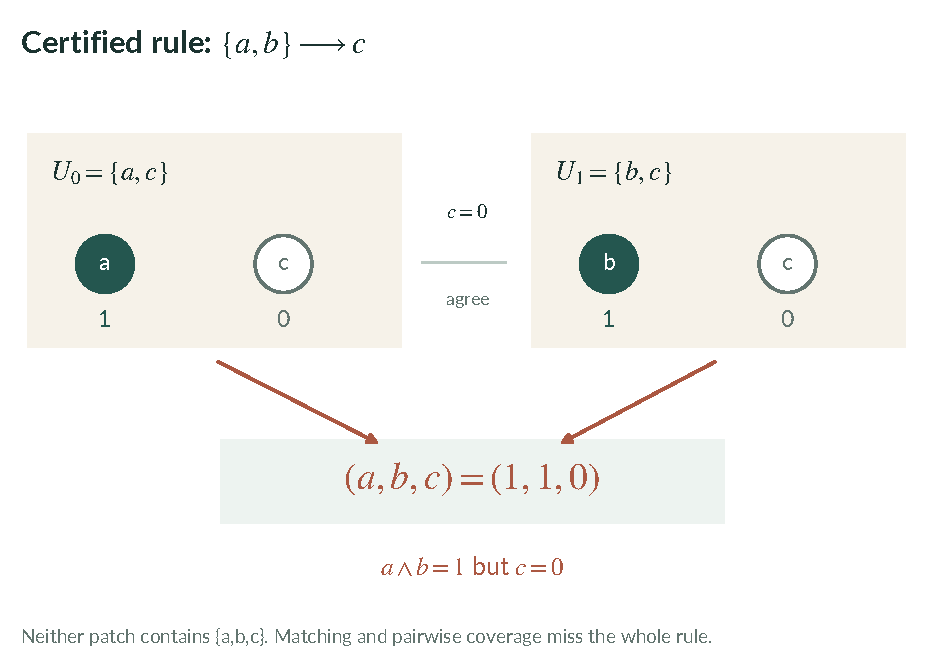
\includegraphics[width=\linewidth]{fig_15_whole_support.pdf}
\caption{The explicit counterexample to replacing whole-support coverage with pairwise dependency coverage. The local data force $(a,b,c)=(1,1,0)$, so both premises hold and the conclusion fails. Green nodes carry value one and open nodes carry value zero.}
\label{fig:whole-support-example}
\end{figure}

{\sffamily\bfseries\color{KomorebiTeal}The successful gluing argument}\par\smallskip
A patch containing the entire support $\{a,b,c\}$ must enforce the conjunctive rule. If all local models match and every certified support occurs in a patch, their union obeys every rule. Node coverage then gives uniqueness. This is the content of Theorem~\ref{thm:support-gluing}, not an inference from pairwise agreement alone.

\medskip
The cover condition is sufficient for all matching data. It need not be necessary for an individual field whose other rules already make a support constraint redundant.
\clearpage

\subsection{Protected realization over a field}

The exact binary model admits a general algebraic formulation. Let $K$ be a field, let $E,R,S$ be $K$-vector spaces, and let $D:E\to R$ and $p:E\to S$ be linear. The prescribed problem is to repair $x$ while retaining $p(x)$:
\[
Dy=0,\qquad p(y)=p(x).
\]
The admissible correction image is $B=D(\ker p)$. The elementary correction equivalence gives feasibility exactly when $Dx\in B$.

\begin{theorem}[A linear certificate alternative]
\label{res:24:5}
\label{thm:linear-alternative}
The protected problem is infeasible if and only if there is a linear functional $\lambda:R\to K$ satisfying
\[
\lambda(Dh)=0\quad\text{whenever }p(h)=0,
\qquad \lambda(Dx)=1.
\]
For a finite matrix $M$ and right side $b$, the corresponding alternative is
\[
\nexists y\ (My=b)
\quad\Longleftrightarrow\quad
\exists\ell\ (\ell M=0\ \text{and}\ \ell b=1).
\]
\end{theorem}
\begin{proof}
If $Dx\notin B$, linear separation of a vector from a subspace gives a functional vanishing on $B$ and nonzero at $Dx$. One construction extends a basis of $B$ by $Dx$ and then to a basis of $R$. Assign value zero to the basis of $B$ and value one to $Dx$, and extend linearly. Equivalently, normalize any separating functional by its nonzero value. Conversely, if $y$ were feasible, then $h=x-y$ would satisfy $p(h)=0$ and $Dh=Dx$, contradicting the displayed functional equations. For a matrix, take $B$ to be its column image. In finite coordinates the separating functional is a row vector, giving the stated alternative.
\end{proof}

The general existence proof is classical. It does not claim an efficient procedure for arbitrary infinite spaces. In the implemented binary case, Gaussian elimination constructs a row witness, and the witness is checked against the original matrix and right side. A positive solution and a normalized negative witness cannot both verify.


\studyhead{03}{An obstruction is a checkable equation}
In the binary example from \path{data/bridge_examples.json}, compatibility demands $a+b=0$ while the protected observations require $a=0$ and $b=1$. The variable $c$ is unconstrained. Its freedom cannot remove the incompatible requirement on the first two coordinates.

\begin{figure}[H]\centering
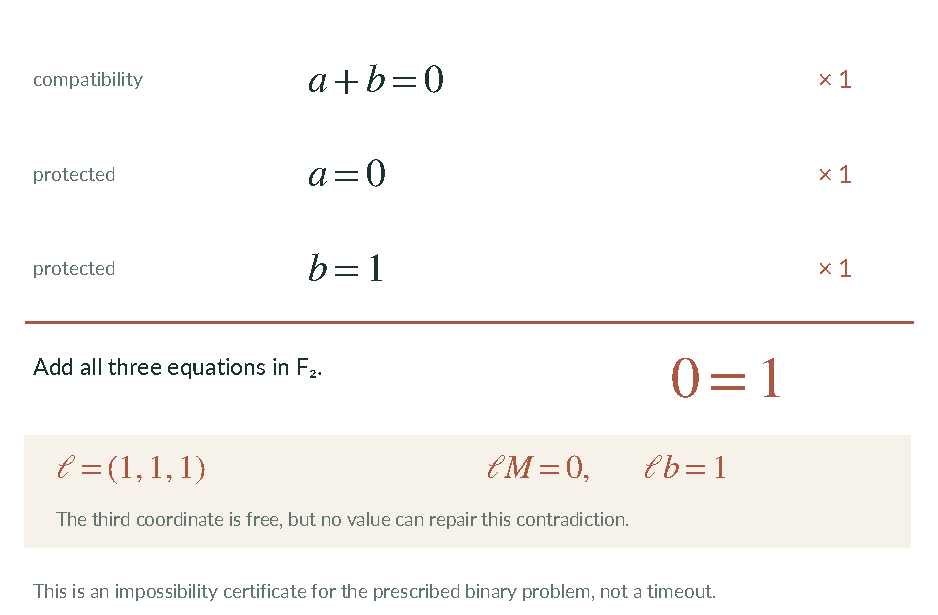
\includegraphics[width=\linewidth]{fig_19_obstruction_witness.pdf}
\caption{A normalized negative witness in $\mathbb F_2$. Adding the three rows gives zero on the left and one on the right. The witness is $\ell=(1,1,1)$, which satisfies $\ell M=0$ and $\ell b=1$ for the original stacked system.}
\label{fig:obstruction-witness}
\end{figure}

The exact system and witness can be inspected without trusting a search procedure:
\[
 M=\begin{pmatrix}1&1&0\\1&0&0\\0&1&0\end{pmatrix},\qquad
 b=\begin{pmatrix}0\\0\\1\end{pmatrix},\qquad
 \ell M=(0,0,0),\quad \ell b=1.
\]
If $My=b$ had a solution, multiplying by $\ell$ would give $0=1$. This is a certificate for the declared protected problem. A search that merely stops supplies no comparable implication.
\clearpage

\subsection{Counting what remains after an observation}

Let $T:E\to R$ and $Q:E\to W$ be linear, and fix a known point $x_0$. Put
\[
\mathcal A=\{y:Ty=Tx_0\},\quad H=\ker T,\quad
Q_H=Q|_H.
\]
Translation $h\mapsto x_0+h$ identifies $H$ with $\mathcal A$. The observation image is the translate $Qx_0+Q(H)$, and the fiber above the attained value $Qx_0$ is a translate of $\ker Q_H$.

\begin{theorem}[Exact observation counts]
\label{res:24:6}
\label{thm:checked-counts}
Suppose $K$ is a finite field of cardinality $q$ and $E$ is a finite-dimensional $K$-vector space. Set
$k=\dim_K H$ and $r=\dim_K Q(H)$. Then
\[
|\mathcal A|=q^k,\qquad
|Q(\mathcal A)|=q^r,\qquad
|\{y\in\mathcal A:Qy=Qx_0\}|=q^{k-r}.
\]
In particular the exact count identity is
\[
|\mathcal A|=
|\{y\in\mathcal A:Qy=Qx_0\}|\,q^r.
\]
Every attained observation fiber has the same size. For the uniform distribution on $\mathcal A$, the observation removes exactly $r\log_2q$ bits of uncertainty.
\end{theorem}
\begin{proof}
The two translation equivalences reduce the counts to finite vector spaces. Such a space of dimension $d$ has $q^d$ elements. Rank-nullity for $Q_H$ gives $\dim\ker Q_H+r=k$, proving the product identity and all the counts. An attained value can be treated by choosing a point attaining it as the base point. Equal fiber sizes imply a uniform observation distribution and a uniform conditional distribution on each fiber. The entropy difference is therefore $\log_2(q^k)-\log_2(q^{k-r})=r\log_2q$.
\end{proof}

Lean checks the translation equivalences, rank-nullity specialization, fiber cardinalities, and product identity in \path{ProofPath.Protected}, with the binary specialization in \path{ProofPath.Binary}. The logarithmic entropy interpretation is the written corollary above, not a newly compiled theorem about a Lean probability distribution. Uniformity is substantive. With a nonuniform prior, dimension alone does not determine Shannon information.

For the protected problem, set $T=(D,p)$ and choose an actual feasible $y_0$, so $Ty_0=(0,px)$. This reduces its solution fiber to the theorem without changing the protected values. A concrete binary example has $a+b+c=0$ and $a=0$. Its two realizations are $(0,0,0)$ and $(0,1,1)$. Observing $b$ has rank one on the ambiguity space and determines the remaining coordinate. Repeating the same observation in two output rows does not double the information.


\studyhead{04}{Ask what an observation distinguishes}
Return to the two vertices $000$ and $011$ from the opening cube. The ambiguity space is the span of $011$. Reading the protected coordinate $a$ repeats known information. Reading $b$ separates the two points. Reading $b$ twice creates two output rows but no additional distinction.

\begin{figure}[H]\centering
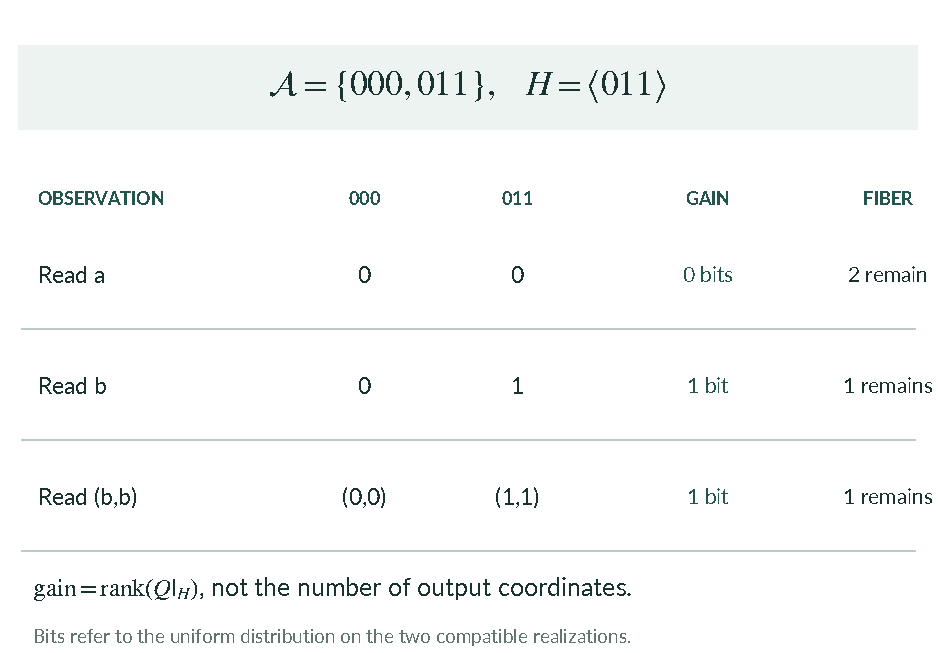
\includegraphics[width=\linewidth]{fig_18_observation_partitions.pdf}
\caption{Three observation maps on the same feasible binary fiber. The last column is the size of each attained conditional fiber. Gains of zero, one, and one bit follow from the rank of the map restricted to $H$, under the uniform distribution. The duplicated output is not twice as informative.}
\label{fig:observation-partitions}
\end{figure}

For example, the repeated observation has matrix
\[
 Q=\begin{pmatrix}0&1&0\\0&1&0\end{pmatrix}.
\]
Its two rows are identical. On $H=\langle011\rangle$ it has rank one, so $|\mathcal A|=2$, $|Q(\mathcal A)|=2$, and every attained observation fiber has size one. These are count identities before they are interpreted probabilistically.

\medskip
The general finite-field formula in Theorem~\ref{thm:checked-counts} retains the same separation: $q^k$ initial possibilities, $q^r$ attained outcomes, and $q^{k-r}$ realizations per outcome.
\clearpage

\subsection{Executable witnesses and a native declaration export}

Four exact examples are regenerated from the Python implementation: a one-bit ambiguity, an incompatible protected assignment, a redundant observation, and a uniquely determined realization. The generator emits the original stacked matrices and right sides alongside the proposed solutions or row witnesses. It also emits Lean declarations which check those concrete equations and cardinalities by kernel reduction. A faulty generator cannot make a false displayed proposition pass merely by assigning a certification flag. The generator itself is not thereby verified for arbitrary inputs, and the correspondence between the supplied JSON input and its emitted Lean syntax remains an audited software boundary.

A separate native exporter reads five already compiled Lean declarations, extracts their direct type and proof-constant dependencies, and records the transitive axiom sets. Dependencies outside the selected roots are explicit external leaves. This yields an actual proof-field JSON record rather than a hand-authored imitation of one. The exported field is then loaded through the public Python importer, and its declared closure is checked to contain its roots.

The export has a deliberately narrow meaning. It is syntactic dependency data for selected declarations, not a reconstruction of the entire discovery process. It does not recover failed attempts, prove that every constant in a type was a historically essential idea, or formally verify the metaprogram that extracts the data. The mathematical proof-field bridge is checked independently of that metaprogram. Its semantic interpretation retains the explicit hypotheses in Theorem~\ref{thm:relative-completeness}.

\subsection{Verification scope and reproducibility}

The present release freshly builds eighteen production Lean modules in a new object directory. Each module is replayed through Lean's own kernel against the pinned imported environment. The nine dependency revisions and the compiler hash are checked before building. All explicit named source declarations receive an axiom audit against the declared whitelist. The thirteen preceding mathematical modules are unchanged. Five new modules add executable trace checking, finite witness completeness, a typed JSON codec, and checked exchange examples.

Ten deliberately invalid files test false conclusions, missing support, placeholders, invalid decoders, merged observations, forged or incomplete closures, and a Boolean used as a node index. A further file introduces an explicit false axiom. Lean correctly accepts a consequence relative to that axiom, while the release's separate axiom policy rejects the dependency. A missing import, unavailable decision procedure, or timeout does not count as a mathematical rejection.

The fresh record is in \path{evidence/formal_1.8.0/}. The older record remains separately identified. Kernel replay here is not an independent implementation of Lean and does not rebuild or replay the entire cached Mathlib library. Written proofs, general Lean statements, generated concrete examples, and Python tests remain different evidence categories. In particular, a sound mathematical algorithm does not make its Python implementation universally verified.

\subsection{Protected extensions of the actual rule field}
\label{sec:protected-rule-extension}

The linear model is not the only setting in which an obstruction can be returned explicitly. The original rule field has its own constructive extension problem. A partial Boolean description records which nodes must belong to a model and which must remain absent. These are observations about the declared model, not assertions that the sentences attached to the nodes are true or false in an intended mathematical universe.

Fix the field $F$, including its admitted leaves and certified rules. For a positive observation set $S\subseteq V$, let
\[
  \operatorname{cl}_F(S)=\operatorname{Der}_{F[S]},
\]
where $F[S]$ is obtained by admitting $L\cup S$ as leaves and changing nothing else. For a negative observation set $N\subseteq V$, define
\[
 \operatorname{Ext}_F(S,N)=
 \{X\subseteq V:X\text{ is an }F\text{-model},\ S\subseteq X,\ X\cap N=\varnothing\}.
\]
Positive and negative observations are both part of the preservation contract. Dropping the negative observations can turn an impossible request into a different, feasible problem.

\begin{theorem}[Least protected extension and a complete obstruction]
\label{res:new:extension}
The extension fiber is nonempty exactly when
\[
 \operatorname{cl}_F(S)\cap N=\varnothing.
\]
When this condition holds, $\operatorname{cl}_F(S)$ is its least member. More generally,
\[
 X\in\operatorname{Ext}_F(S,N)
 \quad\Longleftrightarrow\quad
 X\text{ is an }F\text{-model and }
 \operatorname{cl}_F(S)\subseteq X\subseteq V\setminus N.
\]
If no extension exists, some $n\in N$ has a derivation from $L\cup S$ using only the declared certified rules.
\end{theorem}
\begin{proof}
Induction on a derivation shows that every model containing $S$ contains $\operatorname{cl}_F(S)$. The inductive closure is itself a model and contains $S$. If it avoids $N$, it is therefore a permitted extension, and the preceding inclusion proves leastness. If it meets $N$, every model containing $S$ contains a forbidden node, so no extension is possible. The displayed classification follows from the same inclusions. A point of the nonempty intersection is exactly the conclusion of the stated forbidden-node derivation.
\end{proof}

This describes an interval \emph{inside the family of rule models}, not an arbitrary interval of the power set. Closure under the rules remains essential. Nor is the fiber generally an affine space. For the rule $\{a,b\}\to c$, with no leaves, $S=\varnothing$ and $N=\{c\}$, the allowed models are precisely $\varnothing$, $\{a\}$, and $\{b\}$. There are three, not a power of two. The rank and entropy formulas for vector spaces cannot be imported into this model without additional structure.

\begin{corollary}[Exact extension of a partial valuation]
\label{res:new:partial}
Let $S\subseteq U\subseteq V$. A global model whose true nodes on $U$ are exactly $S$ exists if and only if
\[
 \operatorname{cl}_F(S)\cap U=S.
\]
\end{corollary}
\begin{proof}
Set $N=U\setminus S$. Closure always contains $S$, so avoiding $N$ is equivalent to the displayed equality. Apply Theorem~\ref{res:new:extension}.
\end{proof}

In particular, the test works for partial data that already violate a local rule. It need not assume local consistency and then hide that failure in a precondition. A contradictory observation can be exposed as a specific forbidden consequence.

\begin{proposition}[Staged closure and persistent obstructions]
\label{res:new:stages}
For positive sets $S,T$,
\[
 \operatorname{cl}_F\bigl(\operatorname{cl}_F(S)\cup T\bigr)
   =\operatorname{cl}_F(S\cup T).
\]
If $S\subseteq S'$ and $N\subseteq N'$, then
$\operatorname{Ext}_F(S',N')\subseteq\operatorname{Ext}_F(S,N)$.
Consequently an infeasible request stays infeasible under those additions, while the field and the meaning of its rules remain fixed.
\end{proposition}
\begin{proof}
Closure is extensive, monotone, and idempotent because it is the least model containing its seed. The model $\operatorname{cl}_F(S\cup T)$ contains $\operatorname{cl}_F(S)$ and $T$, giving one inclusion in the first equation. Extensivity gives $S\cup T\subseteq\operatorname{cl}_F(S)\cup T$, and monotonicity gives the other. A model satisfying the larger positive and negative prescriptions also satisfies the smaller ones. The last conclusion follows by inclusion of the extension fibers.
\end{proof}

The module \path{ProofPath.Extension} checks these statements on the existing \path{Field} type. The Python module \path{extension.py} uses the same \path{ProofFieldViews} snapshot as the local-model construction. It computes closure by forward rule scans and records each newly derived node. At most $|V|$ successful insertions occur. If a forbidden node is reached, a causal subtrace is extracted. It need not be the shortest or cheapest refutation.

The independent result checker replays that trace and checks that the recorded closure is closed under every rule. Derivability of every recorded node and closure of the recorded set together establish leastness. A negative witness only needs a valid derivation of one forbidden node. Its replay permits a previously derived node to have become an admitted observation, so the same witness can remain valid after positive data are strengthened. The checker does not call the producer, and a timeout is never returned as an obstruction.


\begin{figure}[htbp]\centering
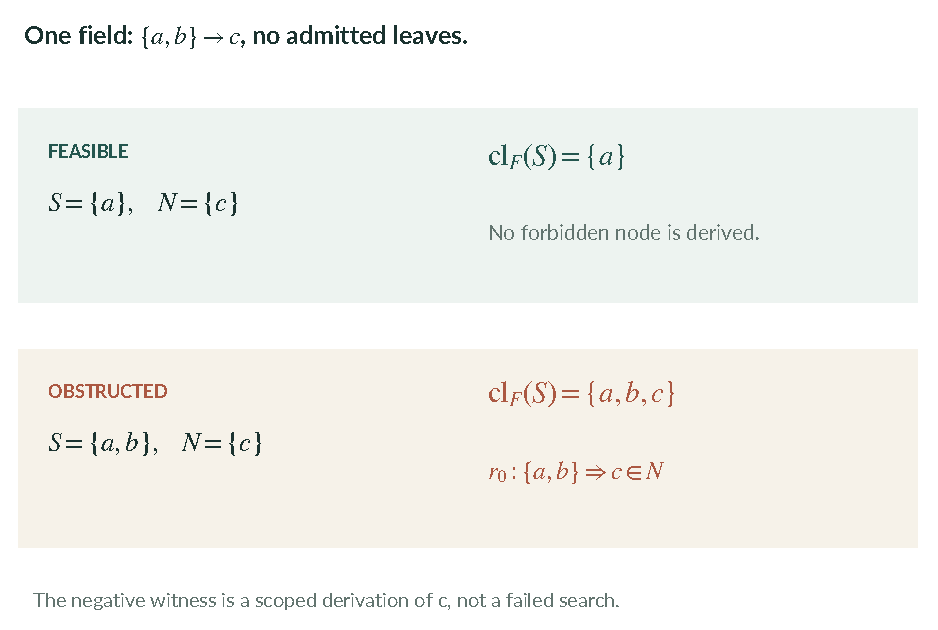
\includegraphics[width=\linewidth]{fig_23_protected_closure.pdf}
\caption{Two protected requests for the same rule field. With only $a$ prescribed true and $c$ prescribed false, the least model is $\{a\}$. Adding $b$ to the positive data derives the forbidden node $c$. The obstruction is the certified rule application, not the act of abandoning a search.}
\label{fig:protected-closure}
\end{figure}

\subsection{Semantic covers rather than only syntactic covers}
\label{sec:semantic-cover}

Whole-support coverage is easy to inspect and is sufficient for gluing. It can nevertheless be unnecessarily strong. Suppose $F$ contains $a\to b$, $b\to c$, and $a\to c$, with patches $\{a,b\}$ and $\{b,c\}$. The last support $\{a,c\}$ is absent from both patches. Yet the first two visible rules already imply the last rule. Requiring another patch would duplicate information rather than restore a missing constraint.

Let $\mathcal U=(U_i)_i$ cover every node. Define $F_{\mathcal U}$ to have the same nodes and leaves as $F$ but only those certified rules whose entire support lies in some $U_i$. The distinction between the two fields is explicit. We call the cover \emph{semantically sufficient for the declared rules} when
\[
 \forall j\text{ certified in }F,\qquad
 c_j\in\operatorname{cl}_{F_{\mathcal U}}(A_j).
 \tag{SC}\label{eq:semantic-cover}
\]
The word semantic here refers to the Boolean rule-model semantics of Section~\ref{sec:old24}, not to an automatic interpretation of node labels as arbitrary mathematical truths.

\begin{theorem}[Exact criterion for universal gluing]
\label{res:new:semantic-cover}
Under node coverage, the following conditions are equivalent:
\begin{enumerate}[label=(\roman*)]
\item Every matching family of local $F$-models on the patches has a unique global $F$-model extending it.
\item Every model of $F_{\mathcal U}$ is a model of $F$.
\item Condition~\eqref{eq:semantic-cover} holds.
\item For every positive seed $S$, $\operatorname{cl}_{F_{\mathcal U}}(S)=\operatorname{cl}_F(S)$.
\end{enumerate}
Whole-support coverage implies these conditions, but the converse need not hold.
\end{theorem}
\begin{proof}
A matching family assembles uniquely to a subset $X\subseteq V$ because the patches cover all nodes and agree on their common coordinates. Its local rule conditions say exactly that $X$ is a model of $F_{\mathcal U}$. Conversely, a model of $F_{\mathcal U}$ restricts to an $F$-model on every patch: every original rule supported in that patch is among the retained rules. Those restrictions match. Thus (i) and (ii) are equivalent, and uniqueness follows from node coverage.

Assume (ii) and fix a certified rule $j$. The set $\operatorname{cl}_{F_{\mathcal U}}(A_j)$ is a model of $F_{\mathcal U}$ containing all of $A_j$. By (ii) it obeys the original rule and contains $c_j$, proving (iii). Conversely, if $X$ is a model of $F_{\mathcal U}$ containing $A_j$, leastness gives $\operatorname{cl}_{F_{\mathcal U}}(A_j)\subseteq X$. Condition (iii) therefore forces $c_j\in X$. Every original rule is satisfied, which proves (ii).

Under (ii) the two fields have exactly the same models, since every $F$-model already obeys the retained rules. Their least models containing any seed are equal, giving (iv). If (iv) holds, apply it to $A_j$. The conclusion $c_j$ lies in $\operatorname{cl}_F(A_j)$ by the original rule, so it lies in the retained closure as required by (iii). Finally, whole-support coverage retains every certified rule. The three-rule example above proves that this condition is not necessary.
\end{proof}

There is a constructive negative result as well. If (SC) fails for $j$, let
\[
 X=\operatorname{cl}_{F_{\mathcal U}}(A_j).
\]
Then $A_j\subseteq X$ and $c_j\notin X$. The restrictions $X\cap U_i$ are matching local $F$-models, but their only assembled subset violates the original rule. They are a checkable obstruction to \emph{universal gluing for this cover}. They do not show that every matching family on the cover fails.

The module \path{ProofPath.SemanticCover} proves the criterion, including its connection to the actual \path{Local}, \path{Matching}, and \path{gluedValue} constructions. It is not a replacement field chosen only to have a convenient name. The Python producer returns a derivation of each original conclusion from its premises using only visible rules, or the countermodel just described. The verifier replays the positive derivations or checks the negative valuation directly. A new \path{glue_semantic} operation requires the positive certificate. The older \path{glue} method retains its simpler whole-support contract.

\studyhead{05}{A missing support can be redundant}
The patches $U_0=\{a,b\}$ and $U_1=\{b,c\}$ do not contain the support of $a\to c$. Their visible rules $a\to b$ and $b\to c$ nevertheless provide a certified derivation of that implication. Compare this with the missing conjunctive support in Figure~\ref{fig:whole-support-example}: neither visible patch there provides a substitute for $\{a,b\}\to c$.

\begin{figure}[H]\centering
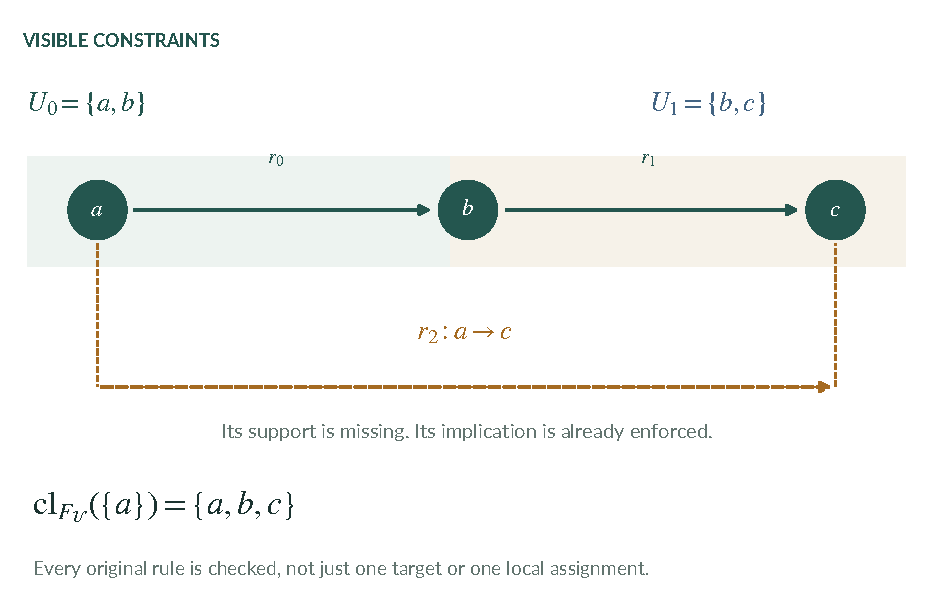
\includegraphics[width=\linewidth]{fig_22_semantic_cover.pdf}
\caption{The exact semantic-cover check for a redundant rule. The two solid rules are visible in the displayed patches. The dashed original rule has no covered whole support, but its conclusion is derived by the solid path. Dashed here means omitted from the visible subsystem, not uncertified in the original field.}
\label{fig:semantic-cover}
\end{figure}

\calloutbox{Preserve the constraint, not necessarily its original presentation}{The cover is sufficient because its visible rules impose the same models as the full field. The criterion checks every original rule, not just the target of one successful example.}

For a finite field, one closure computation per original rule is enough to produce the positive certificates or expose a failed entailment. This avoids enumerating all local valuations or all matching families. The implementation uses repeated rule scans, so the release does not claim the indexed linear-time bound for its code. Its output certificates can be verified without trusting that search procedure.
\clearpage

\subsection{Typed transport of derivations and obstructions}
\label{sec:rule-transports}

A change of proof-field representation needs more than a map of node names. Let $F$ and $G$ be declared fields. A rule transport consists of a node map $f:V_F\to V_G$ and a rule map $h:J_F\to J_G$ satisfying
\[
\begin{aligned}
 f(L_F)&\subseteq L_G,\\
 j\text{ certified in }F&\Longrightarrow h(j)\text{ certified in }G,\\
 A^G_{h(j)}&\subseteq f(A^F_j),\\
 c^G_{h(j)}&=f(c^F_j).
\end{aligned}
\]
The premise inclusion points in the direction needed for executing the translated step. The mapped target rule may need fewer premises, but it must not introduce a new premise unsupported by the source step. This is a sufficient, deliberately concrete transport interface. A more general translation could map one rule to an entire derivation.

\begin{theorem}[Compositional rule transport]
\label{res:new:transport}
Rule transports admit identities and associative composition. A transport $(f,h):F\to G$ sends every derivation of $v$ in $F$ to a derivation of $f(v)$ in $G$. Every $G$-model pulls back along $f$ to an $F$-model. In particular,
\[
 Y\in\operatorname{Ext}_G(f(S),f(N))
   \Longrightarrow f^{-1}(Y)\in\operatorname{Ext}_F(S,N).
\]
An obstruction in the source extension problem therefore implies an obstruction in the target extension problem with the mapped observations.
\end{theorem}
\begin{proof}
Identity maps meet each displayed condition. For two composable transports, compose the node and rule maps. Applying the second map to the first premise inclusion and then using the second inclusion proves the composite premise condition. The conclusion and leaf conditions also compose. Function composition gives the identity and associativity laws.

Proceed by induction on a source derivation. A source leaf maps to a target leaf. For a rule step, every premise of the target rule is the image of a source premise, so the induction hypotheses supply all the required target premises. Certification and the conclusion equation then give the translated conclusion.

If $Y$ is a target model, $f^{-1}(Y)$ contains all source leaves. When it contains every premise of a source rule, $Y$ contains every premise of the mapped rule and hence its conclusion. This proves the model pullback. Positive and negative observations pull back by their image definitions. If a target extension existed while the source problem were infeasible, its pullback would contradict that infeasibility.
\end{proof}

Positive seeds can be added before transport. The same rule transport sends $F[S]$ to $G[f(S)]$, and hence
\[
 f\bigl(\operatorname{cl}_F(S)\bigr)
      \subseteq\operatorname{cl}_G(f(S)).
\]
A forbidden source consequence $n\in N\cap\operatorname{cl}_F(S)$ maps to the explicit forbidden consequence $f(n)\in f(N)\cap\operatorname{cl}_G(f(S))$. The formal development checks this witness map, not only the existence statement obtained by contraposition.

\begin{example}[Why transport is not an equivalence]
\label{res:new:collapse}
Let the source have nodes $a,b$, no leaves, and no rules. The request $a$ true and $b$ false is feasible. Map both nodes to one target node $u$, again with no leaves or rules. This is a rule transport, but the image request requires $u$ both true and false and is infeasible. Thus source feasibility need not imply target feasibility, and target infeasibility need not imply source infeasibility.
\end{example}

\path{ProofPath.RuleTransport} checks these laws for actual derivations, and \path{ProofPath.ExtensionExamples} checks the collapse. The transported conclusion is true under an intended interpretation only if the target leaves and rules are sound. Renaming alone does not provide that contract.


\subsection{Executable certificates for the declared closure}
\label{sec:trace-checker}

A mathematical characterization of closure is not yet a correctness theorem for the program that checks a certificate. The next construction closes that boundary for an explicit Lean checker. It uses the existing \path{Field} and seeded-closure definitions, rather than replacing their meaning by the output of an algorithm.

\begin{definition}[Finite indexed problem and trace]
\label{res:trace:problem}
An indexed problem $P$ specifies a finite address space $V_n=\{0,\ldots,n-1\}$, admitted leaves $L$, a list of certified rules, positive observations $S$, and forbidden nodes $N$. A rule at address $j$ has a finite premise list $A_j$ and conclusion $b_j$. Two identical rows may have different rule addresses. Every listed node must belong to $V_n$. Node lists are individually duplicate free, but $L$, $S$, and $N$ need not be disjoint.

A trace $\sigma=(j_1,\ldots,j_k)$ is a list of rule addresses. Replay begins with the list $K_0=L\mathbin{+\!+}S$. It rejects an unknown rule address or a step whose premises are not all known. Otherwise it adds the conclusion. Strict replay additionally requires the conclusion to be new. Causal replay permits a conclusion already known. Lists are compared by membership when they represent sets.
\end{definition}

Only rows declared certified enter this indexed rule list. The finite checker does not infer certification from a claim's label, its position in a document, or an author's confidence. An adapter that selects these rows must preserve the intended field and its assumptions.

\begin{theorem}[Replay preserves derivability and composes]
\label{res:trace:replay}
Suppose every member of $K$ belongs to $\operatorname{cl}_F(S)$. If either replay mode accepts a trace starting from $K$ and returns $K'$, then
\[
 K\subseteq K'\subseteq\operatorname{cl}_F(S).
\]
For a fixed replay mode, replaying $\sigma\mathbin{+\!+}\tau$ is the same as replaying $\sigma$ and then replaying $\tau$ from the returned state. Failure at either stage propagates to the concatenated execution.
\end{theorem}
\begin{proof}
Induct on the trace. The empty trace returns the initial state. For a nonempty trace, a successful first step identifies a certified rule whose premises are already derivable. Closure under that rule proves its conclusion derivable. Adding the conclusion preserves all previously known nodes, and the induction hypothesis applies to the remaining trace. The stricter novelty test can reject a step but cannot invalidate this argument for an accepted one. The composition identity follows by the same induction, with the lookup and enabling tests taking the same branch on both sides.
\end{proof}

The functions \path{replay}, \path{enabled}, and \path{lookup} are executable definitions. The formal theorems \path{replay_sound}, \path{replay_extensive}, and \path{replay_append} concern those definitions themselves. They are not specifications assumed of an otherwise unchecked replay routine.

\begin{theorem}[Acceptance identifies the least seeded model]
\label{res:trace:least}
A complete-closure certificate consists of a strict trace $\sigma$ and a reported node list $K$. The checker accepts precisely when replay succeeds, its output has the same members as $K$, and $K$ contains the admitted leaves and satisfies every declared rule. Acceptance implies
\[
 \boxed{K=\operatorname{cl}_F(S).}
\]
Here equality means equality of the represented sets, not equality of list order.
\end{theorem}
\begin{proof}
Theorem~\ref{res:trace:replay} gives $K\subseteq\operatorname{cl}_F(S)$ because every initial node is an admitted leaf or a positive observation. Extensivity of replay ensures that $K$ contains $S$. The final closedness test makes $K$ an $F$-model, so leastness of seeded closure gives the reverse inclusion. Both tests are needed: replay provides derivability, while the model test provides saturation under rules not used in the trace.
\end{proof}

The connection to the prior theory is exact. In Lean, \path{closed_iff_model} identifies the Boolean rule check with the existing \path{Field.Model} predicate, and \path{checkClosure_exact} proves the displayed equality with \path{Field.closure}. For a valid indexed problem, \path{valid_closure_bounded} proves that every member of that closure has an address below $n$. Thus totalizing rule lookup in the abstract \path{Field} cannot introduce a conclusion at an unnamed address: only successful lookups are certified.

Logical meaning remains a separate, explicit hypothesis. If an interpretation $\mu:V_n\to\mathrm{Prop}$ satisfies the admitted leaves and rules, and every observation in $S$ is true under $\mu$, then every member of an accepted closure is true under $\mu$. This follows by applying the prior model-soundness theorem to the derived nodes. Acceptance does not establish the truth of arbitrarily attached sentence labels.

\subsection{Finite witnesses for forbidden consequences}
\label{sec:trace-obstruction}

\begin{definition}[Checked forbidden-node witness]
\label{res:trace:witness}
A witness is a pair $(v,\tau)$, consisting of a target address and a causal trace. Its checker accepts when replay from $L\cup S$ succeeds, the returned state contains $v$, and $v\in N$.
\end{definition}

\begin{theorem}[Sound and complete obstruction witnesses]
\label{res:trace:complete}
For the finite-premise indexed rule field,
\[
 \boxed{
 \text{an accepted forbidden-node witness exists}
 \quad\Longleftrightarrow\quad
 \operatorname{Ext}_F(S,N)=\varnothing.
 }
\]
The statement does not require the dependency graph to be acyclic.
\end{theorem}
\begin{proof}
An accepted witness derives a node in $N$. Every model containing $L\cup S$ contains that node, so no protected extension exists.

Conversely, Theorem~\ref{res:new:extension} gives a forbidden node with an inductive derivation. Every such derivation has a finite causal trace. For an admitted leaf or observation, the empty trace suffices. For a rule application, obtain a trace for each of its finitely many premises by induction, concatenate those traces, and append the rule address. Previously derived nodes are never removed. A trace valid from one known set remains valid from a larger known set in causal mode, so the premise traces remain valid when concatenated. Repeated conclusions are allowed, including when an earlier premise trace already established one. The resulting trace derives the forbidden node and is accepted.
\end{proof}

This proof explains the two replay modes. A causal witness can be reused after stronger positive observations make one of its intermediate conclusions already known. Requiring novelty at that point would reject a sound explanation. A complete-closure trace instead records fresh insertions and uses a separate final saturation test. The two contracts should not be conflated.

The Lean development proves trace weakening, strict-to-causal replay, finite premise-trace assembly, and \path{derivation_has_trace} before proving \path{witness_exists_iff_infeasible}. Witness existence is not a claim that a particular search procedure finds the shortest trace, nor is it a bound on the time taken by a Python producer.

\clearpage
\studyhead{06}{Why replay and closedness are both necessary}
\label{study:trace}

Take $V_4=\{0,1,2,3\}$, $L=\{0\}$, $S=\varnothing$, and the two rules $r_0:0\to1$ and $r_1:1\to2$. The least closure is $\{0,1,2\}$. Node $3$ has no derivation from these inputs.

\begin{figure}[H]\centering
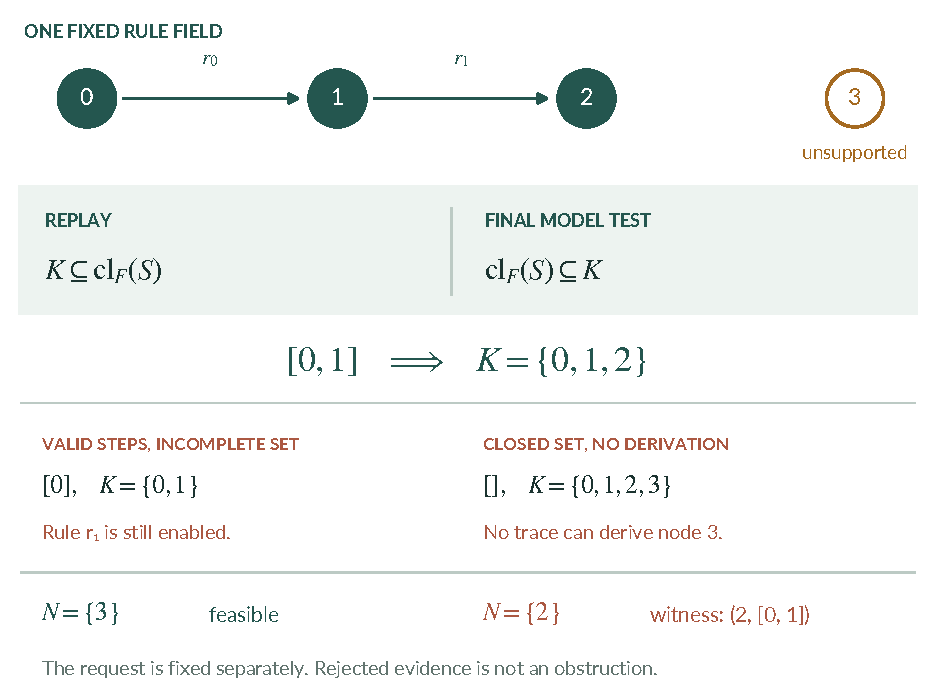
\includegraphics[width=\linewidth]{fig_24_trace_contract.pdf}
\caption{Replay and the final model test establish opposite inclusions. Together they identify the least closure. The two rejected records fail different obligations. Changing only the forbidden set changes the correct feasibility verdict without changing the closure.}
\label{fig:trace-contract}
\end{figure}

The trace $[0]$ derives exactly $\{0,1\}$ but leaves $r_1$ enabled with its conclusion absent. It is a valid partial derivation, not a complete closure. Conversely, $\{0,1,2,3\}$ is closed under both rules, but replay cannot establish its unsupported node $3$. A model need not be the least model.

With $N=\{3\}$, the exact closure gives a positive result. With $N=\{2\}$, the same closure supports a negative result with witness $(2,[0,1])$. The second problem is not a different interpretation of the same request: its protected observations have changed. A checker must receive the fixed request separately from the proposed answer.

\clearpage
\begin{corollary}[Meaning of a complete result certificate]
\label{res:trace:verdict}
The complete result format contains a Boolean feasibility flag, a reported closure, a strict closure trace, and an optional forbidden-node witness. Both branches require the complete-closure check. A positive result additionally requires no obstruction witness and no forbidden node in the closure. A negative result requires an accepted obstruction witness. For every accepted result $C$,
\[
 C.K=\operatorname{cl}_F(S),\qquad
 \bigl(C.\mathrm{feasible}=\mathrm{true}\bigr)
 \Longleftrightarrow
 \operatorname{Ext}_F(S,N)\ne\varnothing.
\]
\end{corollary}
\begin{proof}
The complete-closure check proves the first equality. In the positive branch, the closure is a model containing $S$ and avoiding $N$, hence is an extension. In the negative branch, the witness excludes every extension by Theorem~\ref{res:trace:complete}. Case analysis on the Boolean flag gives the equivalence.
\end{proof}

A bare negative witness has its own checker and does not need a saturated closure. The complete result format asks for both because it promises both an exact closure and a feasibility verdict. Failure of either check means that this certificate was not accepted. It is not itself a refutation of the protected problem.

\subsection{Typed exchange and the boundary of serialization}
\label{sec:trace-wire}

A certificate is useful outside its producer only when the receiving system knows exactly which data it checked. The exchange format therefore uses versioned positional arrays, exact nonnegative integer tokens, literal Booleans, and explicit rule addresses. Problem and certificate are separate records. The node address book and the selected certified-rule order remain associated with the originating proof-field snapshot.

At the JSON syntax-tree level, the problem has the shape
\begin{lstlisting}[language={}]
["proof-path/problem/1", node_count, leaves, rules, positive, negative]
\end{lstlisting}
where each rule is \texttt{[premises, conclusion]}. The certificate has the shape
\begin{lstlisting}[language={}]
["proof-path/certificate/1", feasible, closure, trace, obstruction]
\end{lstlisting}
where an obstruction is either \texttt{null} or \texttt{[target, trace]}. Array lengths and tags are exact. A Boolean is not an integer address, and the string \texttt{"false"} is not a Boolean verdict. Duplicate node entries are rejected by validity checks, while identical rule rows at different addresses remain distinguishable.

\begin{theorem}[Lossless encoding at the typed syntax boundary]
\label{res:trace:codec}
Let $e_P,d_P$ and $e_C,d_C$ be the stated Lean encoders and partial decoders for problem and certificate records. For every typed problem $P$ and certificate $C$,
\[
 d_P(e_P(P))=\operatorname{some}(P),\qquad
 d_C(e_C(C))=\operatorname{some}(C).
\]
Consequently both encoders are injective on their typed domains. These identities do not require the encoded record to pass the separate validity checks.
\end{theorem}
\begin{proof}
The natural-number and Boolean constructors decode to their original values. Induction on a list proves the corresponding array round trip. The rule, witness, and optional-witness decoders then recover their components. Unfolding the exact-length record encoders and decoders gives the two identities. If two encoded records are equal, applying the decoder gives equal \texttt{some} values, hence equal original records.
\end{proof}

\begin{theorem}[Accepted JSON records certify their decoded answer]
\label{res:trace:json}
Suppose the JSON checker accepts the separately supplied problem and certificate syntax trees. Then both decode to typed records $P,C$, both pass their index and shape checks, and the decoded certificate satisfies the closure equality and feasibility equivalence of Corollary~\ref{res:trace:verdict} for that decoded problem.
\end{theorem}
\begin{proof}
The executable checker rejects any failed decoding or validity check. In the remaining branch it calls the same complete result checker used in Corollary~\ref{res:trace:verdict}. Its acceptance therefore supplies that corollary's hypothesis. The round-trip identities additionally show that checking encoded typed records agrees with checking those records directly.
\end{proof}

The general proof ends at Lean's \path{Json} syntax-tree interface. It does not prove the correctness of the standard text parser, printer, file system, Python interpreter, or name-to-index adapter. The command-line reader is executed on actual canonical bytes and compared with an independent finite model oracle. That conformance test complements the formal theorem without extending its quantified scope.

Canonical standalone files use compact ASCII JSON with an optional final newline. Decimal or exponent spellings, alternative internal whitespace, extra fields, and duplicate object-key constructions are outside this exchange contract. The format uses no objects. Resource limits are explicit operational rejections, not evidence that a protected realization is impossible. The encoder's injectivity is a statement about retained data, not a collision-freedom claim for a later cryptographic hash.

The package supplies actual named-field exports, a separate indexed Python checker, the Lean text adapter, and generated Lean fixtures for six concrete exchanges. Their role is to test the entire executed route as well as its proved core. The original named proof fields remain finite and acyclic. Cyclic examples belong to the lower-level indexed checker and show that its soundness theorem does not depend on topological sorting. An unseeded cycle supplies no finite derivation merely by referring to itself.


\monographpart{Compression, representation, and memory}{Compression and memory}{Compression changes which questions can still be answered. A certificate may preserve every required deduction while erasing distinctions that later inquiry needs.}

\section{Compression relative to a task family}
\label{sec:old7}

A representation is sufficient only relative to specified questions and a specified class of possible archives. Fix a set $\mathscr A$ of admissible proof archives. A representation scheme is a map $C:\mathscr A\to\mathscr R$. Its output for an archive $\Pcal$ is $C(\Pcal)$. Distinguishing the scheme from one output is essential: a decoder chosen only after seeing one fixed archive could simply store the answer.

\begin{definition}[Task]
\label{res:7:1}
A task is a map $q:\mathscr A\to Y_q$ to a declared answer set. A task family $\Qcal$ is a set of such maps. Examples include asking for the target certificate, a dependency list, a specified boundary example, or the claims affected by a recorded revision. A teaching or discovery objective becomes an exact task only after its required output or acceptance criterion has been specified.
\end{definition}

\begin{definition}[Task-sufficient representation]
\label{res:7:2}
The scheme $C:\mathscr A\to\mathscr R$ is sufficient for $q$ when there is a single decoder $d_q:C(\mathscr A)\to Y_q$ such that
\[
q(\Pcal)=d_q(C(\Pcal))\qquad\text{for every }\Pcal\in\mathscr A.
\]
It is $\Qcal$-sufficient when this holds for every $q\in\Qcal$. The decoder may depend on the task and the scheme, but not on hidden knowledge of the particular archive being decoded.
\end{definition}

The decoder is defined on attained representations, so no arbitrary answer is required for an encoding that never occurs. Exact reconstruction is one possible task, not a requirement for every purpose. The basic definition is set theoretic and does not assert that a decoder is computable, efficient, or available to a particular reader. Those are additional conditions on a practical compiler.

\begin{theorem}[Task information loss criterion]
\label{res:7:3}
Let $C$ be a compression map and let $q$ be a task. If there exist proof fields $\Pcal_1$ and $\Pcal_2$ such that
\[
C(\Pcal_1)=C(\Pcal_2)
\qquad\text{but}\qquad
q(\Pcal_1)\ne q(\Pcal_2),
\]
then the compressed representation is not sufficient for $q$.
\end{theorem}

\begin{proof}
Suppose a decoder $d_q$ existed. Applying it to the common compressed representation would have to produce both $q(\Pcal_1)$ and $q(\Pcal_2)$. Since these answers differ, no such decoder exists.
\end{proof}

\begin{definition}[Recoverability preorder]
\label{res:7:4}
For a fixed task family $\Qcal$, write
\[
R_1\preceq_{\Qcal} R_2
\]
when every task in $\Qcal$ that factors through the representation scheme $R_1$ also factors through $R_2$. Both schemes have domain $\mathscr A$, and each factorization uses one decoder valid on that whole domain.
\end{definition}

\begin{proposition}[Recoverability is a preorder]
\label{res:7:5}
The relation $\preceq_{\Qcal}$ is reflexive and transitive.
\end{proposition}

\begin{proof}
Every representation supports every task it supports, so the relation is reflexive. If every task supported by $R_1$ is supported by $R_2$, and every task supported by $R_2$ is supported by $R_3$, then every task supported by $R_1$ is supported by $R_3$. Thus the relation is transitive.
\end{proof}

Define $R_1\sim_{\Qcal}R_2$ when both $R_1\preceq_{\Qcal}R_2$ and $R_2\preceq_{\Qcal}R_1$.

\begin{corollary}[Quotient poset]
\label{res:7:6}
The recoverability preorder descends to a partial order on the equivalence classes under $\sim_{\Qcal}$.
\end{corollary}

\begin{proof}
Reflexivity and transitivity pass to equivalence classes. Mutual recoverability has been quotiented out, so antisymmetry holds by construction.
\end{proof}


\subsection{Pure retention operators}

The simplest compression removes nodes without rewriting the retained material. This baseline is useful because it separates information deletion from more complicated summarization or reinterpretation.

\begin{definition}[Retention projection]
\label{res:7:7}
Fix a finite node universe $V$. For a mask $K\subseteq V$, define
\[
P_K(S)=S\cap K,
\qquad S\subseteq V.
\]
\end{definition}

\begin{theorem}[Retention projection algebra]
\label{res:7:8}
For masks $K,L\subseteq V$,
\[
P_K\circ P_L=P_{K\cap L}=P_L\circ P_K.
\]
Consequently every retention projection is idempotent, and the masks form a Boolean lattice with meet $K\cap L$ and join $K\cup L$.
\end{theorem}

\begin{proof}
For every $S\subseteq V$,
\[
P_K(P_L(S))=(S\cap L)\cap K=S\cap(K\cap L).
\]
Intersection is associative and commutative, which gives the composition identity and commutativity. Taking $L=K$ gives idempotence. The power set of $V$ with intersection, union, complement, bottom $\varnothing$, and top $V$ is a Boolean lattice.
\end{proof}

\begin{corollary}[Task monotonicity under retention]
\label{res:7:9}
If $K\subseteq L$, every task whose required nodes and metadata are retained by $P_K$ is also supported by $P_L$.
\end{corollary}

\begin{proof}
Every item retained by $K$ is retained by $L$. Hence every task requirement contained in $K$ is contained in $L$.
\end{proof}

Pure retention operators commute. Noncommutativity in real proof workflows therefore requires an additional operation such as state-dependent summarization, renaming, quotienting, or reinterpretation. This distinction prevents simple deletion from being credited with structure it does not possess.

\begin{figure}[htbp]
\centering
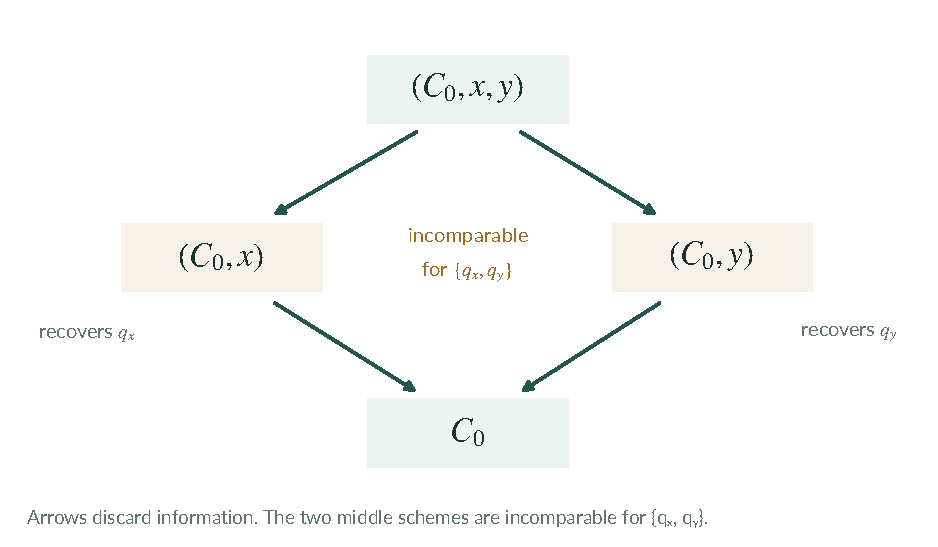
\includegraphics[width=\linewidth]{fig_05_recoverability_preorder.pdf}
\caption{A concrete retention diamond for the four archives $(C_0,x,y)$ with $x,y\in\{0,1\}$. Arrows discard coordinates. The two middle schemes are incomparable for the task family $\{q_x,q_y\}$. This is not a universal ranking of teaching, discovery, and formal presentations.}
\label{fig:preorder}
\end{figure}

\begin{theorem}[Task-family dependence of minimal compression]
\label{res:7:10}
There is a family of archives with a fixed mandatory certificate and two independently variable side records for which different task families have different least sufficient retention masks.
\end{theorem}

\begin{proof}
Let the archives be $\Pcal_{xy}=(C_0,x,y)$ for $(x,y)\in\{0,1\}^2$, where $C_0$ is a fixed certificate retained by every allowed mask. Let $q_x(\Pcal_{xy})=x$ and $q_y(\Pcal_{xy})=y$. Retaining $x$ is sufficient for $q_x$. Any mask omitting $x$ identifies $\Pcal_{0y}$ with $\Pcal_{1y}$, so it is not sufficient for that task. Thus the least mask for $\{q_x\}$ retains exactly $C_0$ and $x$. The same argument gives the least mask $C_0$ and $y$ for $\{q_y\}$. Their joint task family requires both records. These masks are also the unique minima for unit cost per retained side record.
\end{proof}

The example concerns pure retention. A general encoding may recode the records rather than delete them. Sufficiency for all archive queries requires an injective encoding, not literal preservation of the original file. The following theorem makes that distinction precise.

\begin{theorem}[All predicates distinguish exactly injective encodings]
\label{res:7:11}
\label{thm:injective-compression}
Let $C:A\to B$. Every predicate $q:A\to\mathrm{Prop}$ factors through $C$ if and only if $C$ is injective.
\end{theorem}
\begin{proof}
If $C$ is injective, define the decoder of $q$ at $b$ by the predicate $\exists a\ (C(a)=b\ \text{and}\ q(a))$. At $b=C(a_0)$, injectivity makes this equivalent to $q(a_0)$. Conversely, if $C(a)=C(a')$, use the predicate $q(z)\equiv(z=a)$. Its decoded values at the equal encodings must agree, giving $a'=a$. This is the general collision criterion specialized to all predicates.
\end{proof}

The formal result \path{ProofPath.all_predicates_sufficient_iff_injective} records the distinction between information loss and lossless recoding. It makes no assertion about how cheaply a decoder can be computed.


\subsection{A complete factorization test on attained representations}
\label{sec:attained-recovery}

The collision obstruction of Theorem~\ref{res:7:3} has a converse. It gives a complete test for exact task recovery at the level of sets. Write $\operatorname{im}C=C(\mathscr A)$ for the attained output set. A decoder is required on this set and nowhere else.

\begin{theorem}[Attained factorization and unique decoding]
\label{res:new:factorization}
For $C:\mathscr A\to\mathcal R$ and $q:\mathscr A\to Y$, the following are equivalent:
\[
\begin{aligned}
 &\exists d:\operatorname{im}C\to Y\quad
       \forall a\in\mathscr A,\quad q(a)=d(C(a)),\\
 &\forall a,b\in\mathscr A,\quad C(a)=C(b)\Longrightarrow q(a)=q(b).
\end{aligned}
\]
When a decoder exists it is unique on $\operatorname{im}C$. Otherwise there are two archives with the same encoding and different task answers.
\end{theorem}
\begin{proof}
A decoder applied to equal encodings gives equal answers. Conversely, for an attained value $r$, choose $a$ with $C(a)=r$ and define $d(r)=q(a)$. Constancy on each fiber makes the value independent of the choice. At $r=C(a)$ it gives the required answer. Any other decoder must give that same answer at every attained value, proving uniqueness. Negating fiber constancy supplies the pair in the last statement. The construction is set theoretic and uses classical choice in the Lean implementation. It does not provide an efficient decoder for arbitrary infinite archive classes.
\end{proof}

\begin{example}[The empty-domain boundary]
\label{res:new:empty-decoder}
Take $\mathscr A=\varnothing$, $\mathcal R=\{*\}$, and $Y=\varnothing$. There is one encoding and one task on the empty archive class. The attained set is empty, so its empty decoder exists. There is no total decoder $\{*\}\to\varnothing$. Thus attained decoding and decoding on the entire output type are not equivalent without an additional hypothesis.
\end{example}

The earlier formal definition \path{ProofPath.Sufficient} asks for a total decoder. It is retained for compatibility and was not false, but it was stronger than the manuscript's stated domain convention. The new namespace \path{ProofPath.Recovery} matches the manuscript exactly. It proves that total decoding implies attained decoding, and that the two are equivalent whenever the answer type is nonempty. In the latter case choose one default answer for unattained outputs. The empty-domain example is also kernel checked.

The finite Python interface \path{factor_task} takes an explicitly declared table of archive encodings and a task table on the identical domain. It returns either a decoder table or two archive identifiers witnessing a collision. Its verifier checks the proposed result directly, including the empty domain, missing outputs, extra unattained entries, and contradictory records. The table strings are exact identifiers and answers, not a semantic equality procedure for arbitrary mathematical expressions. The existing retention-based \path{task_sufficient} function remains a different, narrower task model.

\subsection{The least information for a family of tasks}
\label{sec:joint-recovery}

Suppose tasks $q_i:\mathscr A\to Y_i$ are indexed by $i\in I$. Their joint representation is
\[
 Q(a)=(q_i(a))_{i\in I}.
\]
It records every distinction asked for by the task family and makes no demand to recover the entire source archive.

\begin{theorem}[Joint task representation and compositional recovery]
\label{res:new:joint}
An encoding $C$ is sufficient for every $q_i$ if and only if it is sufficient for $Q$. In particular every sufficient encoding recovers the joint representation on attained values, while $Q$ itself recovers each task by projection.

If a representation $R$ is recoverable from $C$, then every task recoverable from $R$ is recoverable from $C$. Recovery of representations is reflexive and transitive.
\end{theorem}
\begin{proof}
If $Q$ factors through $C$, each coordinate factors by projection. Conversely, equal values of $C$ give equal values of every $q_i$. Function extensionality gives equal joint vectors, and Theorem~\ref{res:new:factorization} supplies the joint decoder. This argument allows a different answer type for each task and also covers an empty task family.

For the second assertion, write $R=\pi\circ C$ and $q=d\circ R$ on their attained sets. Then $q=(d\circ\pi)\circ C$. The identity decoder proves reflexivity, and composition of two recovery maps proves transitivity. All maps are applied only to outputs in their declared domains.
\end{proof}

The word least concerns retained distinctions, not bytes, running time, or the cognitive cost of reading an archive. Two archives are identified by $Q$ precisely when every declared task gives the same answer on them. Any sufficient representation may retain more, but it cannot identify archives that $Q$ distinguishes. For a finite archive family, the reference implementation labels these joint-answer classes and checks that every task is constant within a class. Costs remain a separate optimization problem.

This result also completes the formal justification of the recovery condition in Section~\ref{sec:old19}. A refinement that reconstructs only the final theorem need not preserve the joint tasks of audit and discovery. A refinement with a checked recovery map for the preceding representation does preserve them. The distinction is between a longer proof and a genuinely more informative archive, not between short and long documents in general.


\section{Endpoint, audit, and discovery equivalence}
\label{sec:old8}

The phrase ``the same proof'' can refer to several distinct equivalence relations.

\begin{definition}[Endpoint equivalence]
\label{res:8:1}
Fix a background theory, an interpretation of claim labels, and an admissible inference policy. Within that context, two representations are endpoint equivalent when they certify the same judgment from the same complete assumption context and requested targets. Required premises and any additional admitted assumptions are accounted for in that context. A comparison across different contexts requires an explicitly specified transport of assumptions and judgments, not merely identical displayed labels.
\end{definition}

\begin{definition}[Audit equivalence]
\label{res:8:2}
Two representations are audit equivalent when they preserve equivalent dependency, evidence, provenance, and scope information for checking the declared targets.
\end{definition}

\begin{definition}[Discovery equivalence]
\label{res:8:3}
Two representations are discovery equivalent relative to a declared bridge model when they preserve the same examples, alternatives, boundary cases, candidate routes, and future reach, up to the chosen graph equivalence.
\end{definition}

When audit and discovery task families are required to include the endpoint tasks, either equivalence implies endpoint equivalence. Audit and discovery equivalence need not imply one another: a representation may preserve provenance without alternatives, or alternatives without provenance. Their joint task family is stronger than either. Any further hierarchy requires an explicit inclusion of task families. Two perfectly valid certificates can therefore expose different mathematical neighborhoods without differing in validity.

\begin{remark}
\label{res:8:4}
These equivalences are task-relative. Discovery equivalence requires a declared bridge model. It is not an assertion that every future use of a proof can be predicted.
\end{remark}


\section{Vector-valued loss}
\label{sec:old9}

Let a node $v$ carry finite nonnegative numerical coordinates
\[
\mathbf v(v)=
\bigl(V(v),D(v),M(v),F(v),A(v)\bigr),
\]
representing declared verification, discovery, meaning, future bridge, and auditability weights. Summation requires an additive numerical model. The weights may be supplied or estimated, but an ordinal ranking alone does not justify adding them. Changing a numerical scale can change the resulting loss and retention problem.

\begin{definition}[Additive loss vector]
\label{res:9:1}
For a retained node set $K\subseteq V$, define
\[
\Loss(\Pcal,K)
=
\sum_{v\notin K}\mathbf v(v).
\]
Normalize a coordinate by its total only when that total is positive. If the total is zero, nonnegativity makes every contribution in that coordinate zero. The implementation records normalized loss zero there as a convention, rather than dividing by zero.
\end{definition}

\begin{proposition}[Zero verification loss can coexist with positive discovery loss]
\label{res:9:2}
There exist proof fields and certificates $K$ for which the verification coordinate of $\Loss(\Pcal,K)$ is zero while the discovery and bridge coordinates are positive.
\end{proposition}

\begin{proof}
Take an AND-DAG certificate from $A$ to $B$ and add an optional example node $E$ that is not an ancestor of $B$. Assign positive discovery and bridge values to $E$ and zero verification value. The unique core omits $E$ while preserving the entire verification ancestry. The verification loss is zero and the other declared losses are positive.
\end{proof}

\begin{figure}[htbp]
\centering
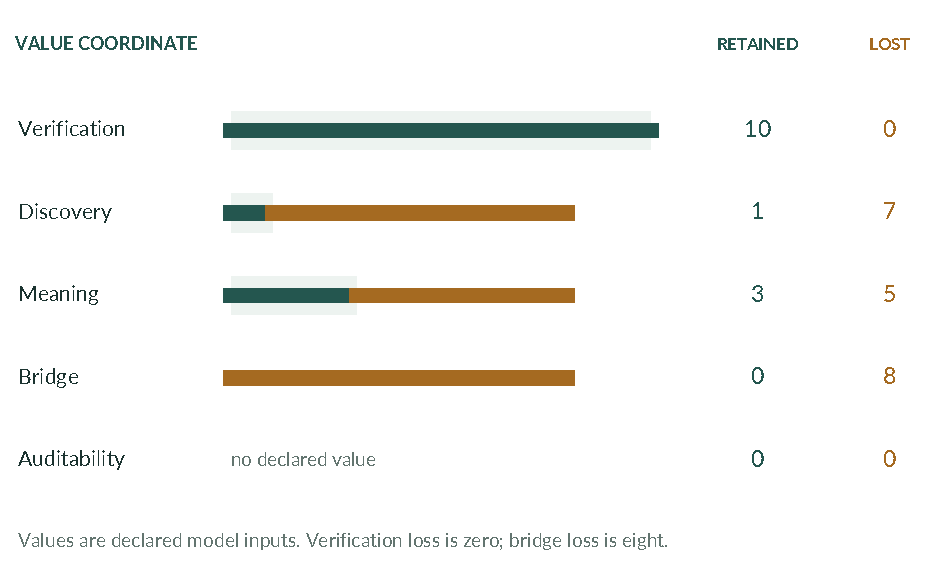
\includegraphics[width=\linewidth]{fig_06_loss_vectors.pdf}
\caption{Exact retained and lost values for the canonical AND-DAG certificate. The numbers are declared values, not measured universal units of meaning. Zero verification loss coexists with loss of seven discovery units and eight bridge units. All auditability values in this example were declared zero.}
\label{fig:loss}
\end{figure}

No claim is made that all value coordinates are additive. Additivity is a transparent baseline. Interactions can be represented by hyperedge values, submodular utilities, or task-specific decoders when the application requires them.


\section{Compression debt}
\label{sec:old10}

Compression may postpone work rather than eliminate it. A later task may require reconstruction of material that was omitted from the current representation.

\begin{definition}[Future task model]
\label{res:10:1}
Let $\Tcal$ be a finite task set with probabilities $p_t\ge0$ satisfying $\sum_t p_t=1$. Let $R_t\subseteq V$ be the node set required by task $t$, and let $c(v)\ge0$ be the recovery cost of node $v$ when it is absent.
\end{definition}

\begin{definition}[Expected compression debt]
\label{res:10:2}
The expected compression debt of retained set $K$ is
\[
\Debt(K)
=
\sum_{t\in\Tcal}p_t
\sum_{v\in R_t\setminus K}c(v).
\]
\end{definition}

\begin{proposition}[Debt is monotone under retention]
\label{res:10:3}
If $K_1\subseteq K_2$, then
\[
\Debt(K_2)\le\Debt(K_1).
\]
\end{proposition}

\begin{proof}
For every task $t$, the missing set $R_t\setminus K_2$ is contained in $R_t\setminus K_1$. Recovery costs are nonnegative. The taskwise cost cannot increase, and neither can its probability-weighted sum.
\end{proof}

\begin{corollary}[Irreversible compression accumulates debt]
\label{res:10:4}
For a descending sequence of retained sets
\[
K_0\supseteq K_1\supseteq\cdots\supseteq K_r,
\]
the expected debt is nondecreasing.
\end{corollary}

A recovery archive can change the cost function. If an omitted node has a stable provenance pointer and a reproducible generator, its recovery cost may be small. If it survives only in memory, its recovery cost may be effectively infinite.


\section{A proof ecology rather than one ideal form}
\label{sec:old11}

The same theorem can support several legitimate representations:
\[
\Rcal(B)=
\{R_{\mathrm{cert}},R_{\mathrm{journal}},R_{\mathrm{teach}},
R_{\mathrm{formal}},R_{\mathrm{discovery}},R_{\mathrm{archive}}\}.
\]
The certificate is optimized for checking. The journal form balances rigor and readable length. The teaching form expands conceptual bottlenecks. The formal form exposes primitive dependencies. The discovery form retains alternatives and failed routes. The archive preserves reconstruction information.

\begin{definition}[Representation portfolio]
\label{res:11:1}
A representation portfolio is a family of proof representations together with stable claim identifiers, translation maps, and a shared status ledger.
\end{definition}

\begin{proposition}[Portfolio robustness]
\label{res:11:2}
For representation schemes $C_i:\mathscr A\to R_i$, retain the tagged portfolio $C(\Pcal)=(C_i(\Pcal))_i$. Every task recoverable from any one $C_i$ is recoverable from $C$.
\end{proposition}

\begin{proof}
If $q=d_i\circ C_i$, compose $d_i$ with the $i$th coordinate projection from the portfolio. This gives a decoder of $q$ from $C$. Retaining the coordinate labels is part of the construction. An untagged union that loses source identities need not permit the same recovery.
\end{proof}

Redundancy is useful when it is heterogeneous. Storing six copies of the same compressed certificate adds little. Storing a certificate, an expanded explanation, a formal dependency graph, and a reproducible notebook may preserve genuinely different values.


\section{Proof compilers and shared ledgers}
\label{sec:old12}

A proof compiler generates a representation for a specified purpose from one canonical proof field. The connection between source and readable exposition also motivates literate programming \cite{knuth}.

\begin{definition}[Proof compiler]
\label{res:12:1}
Let $g$ be a presentation goal and let $\Pcal$ be a versioned proof field. A proof compiler is a map on the declared archive class
\[
\Gamma_g:\mathscr A\longrightarrow R_g
\]
that selects, orders, and renders the material required by $g$ while preserving links to canonical claim and justification identifiers.
\end{definition}

Typical goals include certificate, journal, teaching, discovery, formal verification, and archive. The compiler does not invent logical status. It reads status from the canonical ledger.

\begin{proposition}[Shared-ledger consistency]
\label{res:12:2}
Suppose every compiled representation is generated from one canonical ledger and every rendered claim retains its ledger identifier. Then a status correction can be propagated consistently to every compiled representation containing that claim by updating the ledger and recompiling.
\end{proposition}

\begin{proof}
The stable identifier determines every occurrence of the claim across the compiled outputs. Updating the canonical record changes the source value associated with that identifier. Recompilation reads the updated record in every view. A stale status can persist only in an output detached from the canonical ledger or not recompiled.
\end{proof}

This proposition is operationally important. A monograph, a formal library, and a teaching site should not maintain independent truth labels for the same claim.


\section{Latent bridge graphs}
\label{sec:old13}

A proof field records certified dependencies. A latent bridge graph records possible future transfers. The two graphs have different logical roles.

\begin{definition}[Latent bridge graph]
\label{res:13:1}
A latent bridge graph is a finite directed graph
\[
\Bcal=(W,E_B)
\]
whose nodes include retained proof objects, omitted proof objects, and anticipated future targets. An edge $x\to y$ means that $x$ has been declared a possible transfer route toward $y$. The edge may be certified, conjectural, or exploratory, but its status must be recorded.
\end{definition}

Let $S\subseteq W$ be the retained starting set. Let $F\subseteq W$ be a future target set with weights $w_f\ge0$.

\begin{definition}[Future reach utility]
\label{res:13:2}
The weighted future reach of $S$ is
\[
U(S)=\sum_{f\in F}w_f\,
\mathbf 1\{f\in\Reach_{\Bcal}(S)\}.
\]
\end{definition}

This quantity measures declared reach, not truth. A conjectural edge can increase modeled reach without certifying the target. The ledger must keep those statuses separate.

\subsection{Bridge criticality and dominators}

\begin{definition}[Bridge-critical node]
\label{res:13:3}
A node $v$ is bridge critical for target $f$ relative to starts $S$ when $f$ is reachable from $S$ in $\Bcal$ and becomes unreachable after $v$ is removed.
\end{definition}

In graph language, $v$ dominates an initially reachable $f$ relative to $S$ when every directed path from $S$ to $f$ passes through $v$. Paths of length zero are allowed in the reachability convention. Standard graph terminology is used throughout \cite{diestel}.

\begin{theorem}[Criticality equals domination]
\label{res:13:4}
Assume $f$ is reachable from $S$. A node $v\notin S$ is bridge critical for $f$ if and only if $v$ dominates $f$ relative to $S$.
\end{theorem}

\begin{proof}
If $v$ dominates $f$, every path from $S$ to $f$ uses $v$. Removing $v$ removes every such path, so $f$ becomes unreachable. Conversely, if removing $v$ makes $f$ unreachable, then there could not have been a path from $S$ to $f$ avoiding $v$. Therefore every path used $v$, which is exactly domination.
\end{proof}

\begin{corollary}[Weighted criticality]
\label{res:13:5}
For $v\notin S$, the utility lost by deleting $v$ is the total weight of initially reachable future targets dominated by $v$:
\[
U(S)-U_{\Bcal\setminus\{v\}}(S)
=\sum_{\substack{f\in F\cap\Reach_{\Bcal}(S)\\v\text{ dominates }f}}w_f.
\]
Deleted target vertices are counted as unreachable.
\end{corollary}

\begin{figure}[htbp]
\centering
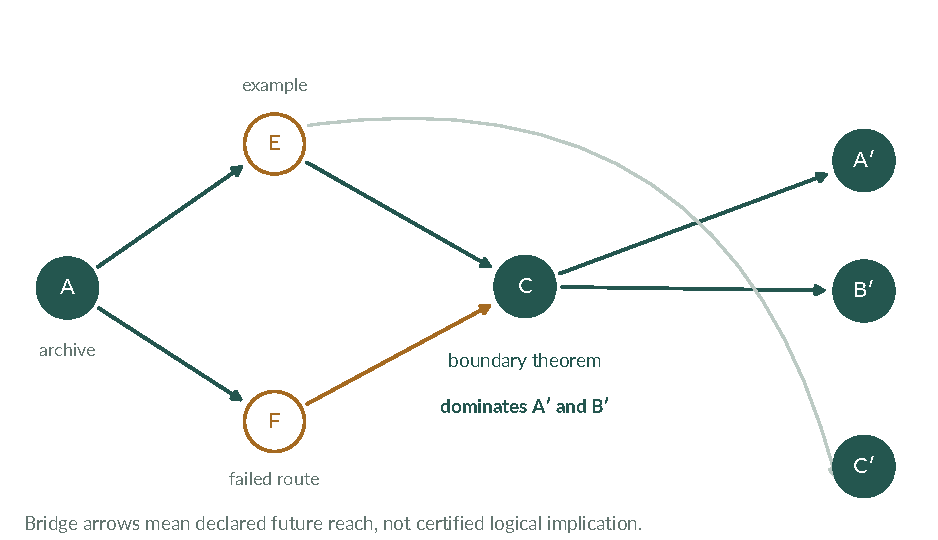
\includegraphics[width=\linewidth]{fig_07_bridge_dominators.pdf}
\caption{A declared bridge graph. The boundary theorem $C$ dominates future targets $A^\prime$ and $B^\prime$ but not $C^\prime$, which has a bypass from $E$. These arrows describe future reach in the supplied model, not proof certification. Deleting a bridge vertex is different from merely retaining a different source set.}
\label{fig:dominator}
\end{figure}

A node may have low verification value for the current theorem and high domination value for future targets. This is the precise form of the claim that a forgotten step can remain mathematically important after it has lost its role in the original certificate.


\section{Retention under a budget}
\label{sec:old14}

An archive cannot retain every object at full resolution. The first mathematically controlled retention problem is to choose a finite supplement that preserves as much future reach as possible.

Let $C\subseteq W$ be the candidate nodes that may be retained and let $M$ be a mandatory base set. For $S\subseteq C$, define
\[
U_M(S)=U(M\cup S).
\]
The bridge graph remains fixed: retention changes the starting set, not the available intermediate vertices or edges. Deleting unretained intermediate vertices would define a different objective, for which the coverage proof below need not apply.

\begin{theorem}[Bridge coverage is monotone and submodular]
\label{res:14:1}
\label{thm:bridge-submodular}
The future reach utility $U_M$ is a nonnegative monotone submodular set function on $C$.
\end{theorem}

\begin{proof}
For each candidate $x\in C$, let $R_x\subseteq F$ be the set of future targets reachable from $M\cup\{x\}$. Let $R_M$ be the targets already reachable from $M$. Reachability from a union of starting nodes is the union of their individual reach sets, so
\[
U_M(S)=
\sum_{f\in R_M\cup\bigcup_{x\in S}R_x}w_f.
\]
Adding a candidate cannot remove a reachable target, so $U_M$ is monotone.

Now let $S\subseteq T\subseteq C$ and let $x\in C\setminus T$. The marginal gain of adding $x$ is the total weight of targets in $R_x$ that are not already covered. Since $T$ covers at least every target covered by $S$, the set newly covered from $T$ is contained in the set newly covered from $S$. Therefore
\[
U_M(S\cup\{x\})-U_M(S)
\ge
U_M(T\cup\{x\})-U_M(T),
\]
which is submodularity.
\end{proof}

\begin{theorem}[Greedy cardinality guarantee]
\label{res:14:2}
\label{thm:bridge-greedy}
Let $k$ be an integer with $1\leq k\leq|C|$. Starting from the empty supplement, let $S_k$ result from repeatedly adding an unselected candidate with largest marginal future reach. Let $O_k$ be an optimal supplement of size at most $k$. Then
\[
U_M(S_k)-U_M(\varnothing)
\ge
\left(1-\left(1-\frac1k\right)^k\right)
\bigl(U_M(O_k)-U_M(\varnothing)\bigr),
\]
and therefore the greedy gain is at least $(1-1/e)$ times the optimal gain.
\end{theorem}

\begin{proof}
Write $G_i=U_M(S_i)-U_M(\varnothing)$ and $G^*=U_M(O_k)-U_M(\varnothing)$. By monotonicity and submodularity, the total marginal contribution of the at most $k$ elements of $O_k$ beyond $S_i$ is at least $G^*-G_i$. Hence at least one candidate has marginal gain at least $(G^*-G_i)/k$. Greedy chooses a candidate with at least that gain, so
\[
G^*-G_{i+1}
\le
\left(1-\frac1k\right)(G^*-G_i).
\]
Iterating from $G_0=0$ gives
\[
G^*-G_k
\le
\left(1-\frac1k\right)^kG^*.
\]
Rearranging gives the first bound. The inequality $(1-1/k)^k\le e^{-1}$ gives the second.
\end{proof}

\begin{warning}[Arbitrary costs]
\label{res:14:3}
For $k=0$, both gains are zero without using the displayed division by $k$. For a budget at least $|C|$, retaining all candidates is optimal. The displayed theorem is the cardinality form of the standard submodular greedy bound \cite{nemhauser}. A gain-per-cost rule for unequal costs is a different algorithm and does not inherit this guarantee. Zero-cost candidates also need an explicit convention.
\end{warning}

\begin{figure}[H]
\centering
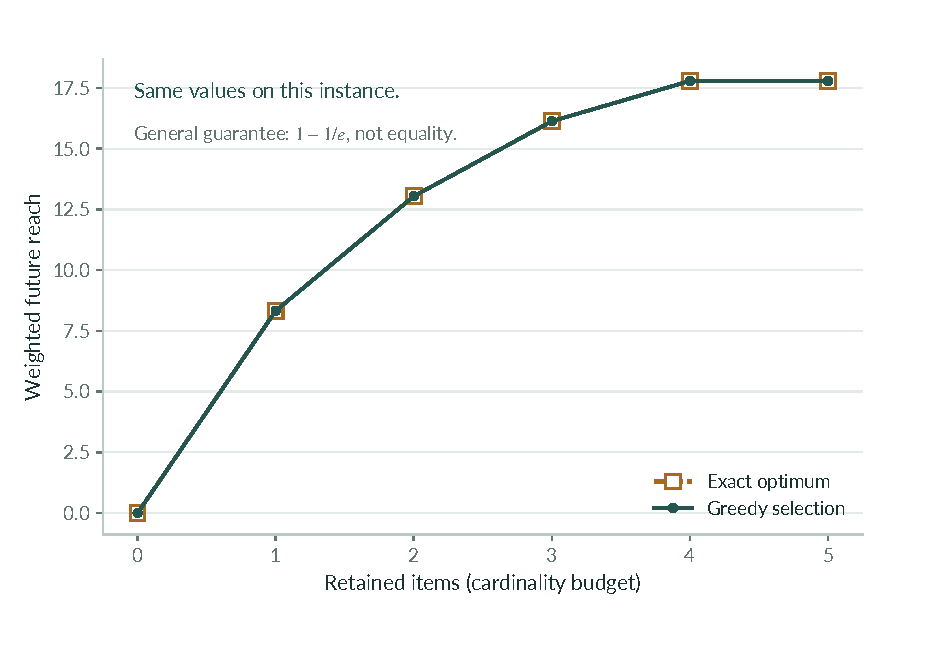
\includegraphics[width=\linewidth]{fig_08_submodular_greedy.pdf}
\caption{Greedy and exact retention coincide on the committed finite instance. The square and circle marks are deliberately overlaid. The general cardinality guarantee is $1-1/e$, not equality with the optimum on every graph.}
\label{fig:greedy}
\end{figure}


\monographpart{Revision, review, and inquiry}{Revision and inquiry}{A mathematical archive has a continuing life. Revisions, shared error, and finite checking capacity change its use without changing the standard of proof.}

\section{Versioned proof objects}
\label{sec:old15}
\label{sec:versioned}

A proof archive changes. Claims are strengthened, corrected, refuted, or split. A reproducible theory therefore needs stable identifiers and explicit version relations.

\begin{definition}[Versioned proof object]
\label{res:15:1}
A versioned proof object is a sequence
\[
\Pcal_0\longrightarrow\Pcal_1\longrightarrow\cdots
\]
whose nodes and justifications carry stable identifiers. Each transition records additions, removals, altered scopes, evidence changes, and a digest of its parent version.
\end{definition}

\begin{definition}[Append-only certified update]
\label{res:15:2}
An update $\Pcal_i\to\Pcal_{i+1}$ is append-only certified when every existing node, admissible-leaf status, evidence record, interpretation, and certified justification remains unchanged. The later field may add records and certified rules but may not withdraw an earlier admitted leaf or change the scope of an earlier inference.
\end{definition}

\begin{theorem}[Derivability is monotone under append-only updates]
\label{res:15:3}
Every target derivable in $\Pcal_i$ remains derivable in $\Pcal_{i+1}$ under an append-only certified update.
\end{theorem}

\begin{proof}
A certificate in $\Pcal_i$ uses only nodes and certified justifications that remain unchanged in $\Pcal_{i+1}$. The same selected subfield therefore satisfies the same derivability closure in the later version.
\end{proof}

Retractions and semantic changes are not append-only. They require invalidation analysis.

\begin{definition}[Syntactic affected set]
\label{res:15:4}
For a changed node set $X\subseteq V$, define
\[
\operatorname{Aff}(X)=X\cup\Desc(X),
\]
where descendants are computed in the declared dependency graph.
\end{definition}

\begin{theorem}[Minimal closed syntactic review set]
\label{res:15:5}
The set $\operatorname{Aff}(X)$ is the unique smallest node set $Y$ such that $X\subseteq Y$ and $Y$ is closed under outgoing dependency edges: whenever $u\in Y$ and $u\to v$ is a declared dependency edge, then $v\in Y$.
\end{theorem}

\begin{proof}
By construction, every node reachable from $X$ lies in $\operatorname{Aff}(X)$, so the set contains $X$ and is closed under outgoing edges. Let $Y$ be any other set with those two properties. Every directed path beginning in $X$ remains inside $Y$ by induction on path length. Hence every descendant of $X$ lies in $Y$, and $\operatorname{Aff}(X)\subseteq Y$.
\end{proof}

\begin{figure}[htbp]
\centering
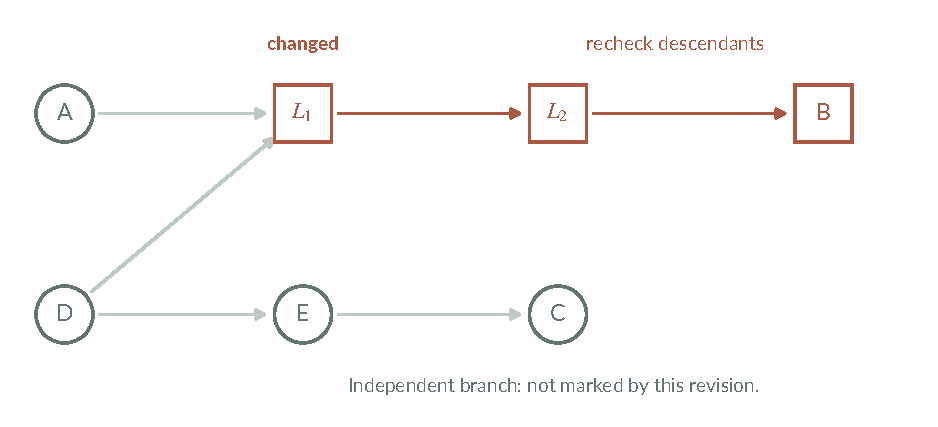
\includegraphics[width=\linewidth]{fig_09_version_invalidation.pdf}
\caption{Changing $L_1$ marks $L_1$, $L_2$, and $B$ for syntactic review. The lower branch has no forward dependency path from $L_1$. Membership in the review set is not a claim that a theorem has become false.}
\label{fig:invalidation}
\end{figure}

The theorem is intentionally syntactic. A descendant can survive after rechecking. The affected set says where review is required, not where falsehood is guaranteed.


\FloatBarrier
\section{Evidence ledgers and provenance}
\label{sec:old16}

\Needspace{9\baselineskip}
A claim ledger should answer five questions without reconstructing the entire research history.

\begin{enumerate}
\item What is the exact claim identifier?
\item What is its current status and scope?
\item Which justifications depend on it?
\item Which evidence records support or challenge it?
\item Which versions and compiled documents contain it?
\end{enumerate}

\begin{definition}[Evidence ledger]
\label{res:16:1}
An evidence ledger is an appendable collection of typed, scoped records linked to claim and justification identifiers. A record may certify, support, challenge, interpret, or refute an object. Its role is explicit rather than inferred from prose placement.
\end{definition}

\begin{definition}[Provenance digest]
\label{res:16:2}
A provenance digest is a cryptographic hash of a canonical serialization of the claim identifier, content, scope, evidence references, parent version, and relevant build inputs.
\end{definition}

A digest does not prove a theorem. A changed digest establishes that the hashed byte sequence changed. An unchanged digest is an integrity check only subject to the possibility of collisions. Canonical serialization gives different representations a common byte-level reference.

\begin{proposition}[Digest stability]
\label{res:16:3}
Fix a deterministic serialization $s$ and a deterministic hash function $h$. Identical serialized byte sequences have identical digests under $h$. Distinct serialized byte sequences have distinct digests unless they form a collision under $h$. Detecting a record change additionally requires that the change alter its serialized bytes.
\end{proposition}

\begin{proof}
If $s(r)=s(r')$, applying the function $h$ gives equal digests. If $s(r)\ne s(r')$ but $h(s(r))=h(s(r'))$, the two serialized strings form a hash collision by definition. Thus change detection at the record level requires both preservation of the audited distinction by $s$ and exclusion of a collision for the resulting bytes. No injectivity of a fixed-length hash on arbitrary byte strings is asserted.
\end{proof}


The serialization contract must state which fields, types, and distinctions it preserves and which differences it intentionally normalizes. Loss during serialization and a collision during hashing are separate mechanisms.

For example, joining string parts with a separator is ambiguous if the same separator may occur inside a part. The tuples $(\texttt{a|b},\texttt{c})$ and $(\texttt{a},\texttt{b|c})$ both become \texttt{a|b|c}. No hash function can recover the lost tuple boundary. The earlier \path{provenance_digest} helper had this defect with a control-character separator. Python release 1.4.0 replaces that encoding with a versioned, domain-separated JSON array of strings. Historical digests must retain their earlier format and version. The snapshot digest has its own unchanged serialization contract.

\begin{proposition}[Hashing cannot add recoverable tasks]
\label{res:new:hash}
Let $s:\mathscr A\to B$ be serialization and $h:B\to D$ be any deterministic map. Every task recoverable from $h\circ s$ is recoverable from $s$. If $h$ is injective on the attained set $s(\mathscr A)$, the two encodings support exactly the same tasks.
\end{proposition}
\begin{proof}
If $s(a)=s(b)$, then $h(s(a))=h(s(b))$. Any task constant on the digest fibers is therefore constant on the serialization fibers, and Theorem~\ref{res:new:factorization} supplies its decoder. If $h$ is injective on attained serializations, equality of digests conversely implies equality of serializations, so the two fiber partitions coincide and the same criterion applies in both directions.
\end{proof}

The module \path{ProofPath.Recovery} checks both implications. The injectivity condition is a conditional mathematical hypothesis, not a claim that a fixed-length cryptographic hash is injective on arbitrary inputs. A hash cannot repair an ambiguity introduced before hashing. It may introduce additional collisions, which must be kept separate from the serializer's preservation contract.

\section{Correlated review}
\label{sec:old17}
\label{sec:correlated-review}

Several reviews are not equivalent to several independent reviews. Reviewers may share training, notation, examples, software, or an unnoticed premise.

Let $X_i=\theta+\varepsilon_i$ be numerical estimates of a fixed quantity $\theta$. Assume $\mathbb E\varepsilon_i=0$, $\operatorname{Var}(\varepsilon_i)=\sigma^2>0$, and common pairwise correlation $\rho$. For $n>1$, assume $-1/(n-1)<\rho\leq1$, so the mean has positive variance. These variables model estimates, not proof truth values. The mean has variance
\[
\operatorname{Var}(\bar X)
=
\sigma^2\left(\frac{1-\rho}{n}+\rho\right).
\]

\begin{theorem}[Effective reviewer count]
\label{res:17:1}
\label{thm:review-count}
Under the equicorrelated model, define the variance-equivalent reviewer count by
\[
\boxed{
 n_{\mathrm{eff}}
 =
 \frac{n}{1+(n-1)\rho}
}
\]
so that $\operatorname{Var}(\bar X)=\sigma^2/n_{\mathrm{eff}}$. This effective count is a positive real number and need not be an integer.
\end{theorem}

\begin{proof}
The mean of $m$ independent reviewers of variance $\sigma^2$ has variance $\sigma^2/m$. Equating this with the correlated mean variance gives
\[
\frac{\sigma^2}{m}
=
\sigma^2\left(\frac{1-\rho}{n}+\rho\right)
=
\sigma^2\frac{1+(n-1)\rho}{n}.
\]
Solving for $m$ gives the formula.
\end{proof}

For $n=1$, the effective count is one. At the excluded boundary $\rho=-1/(n-1)$, the mean has zero variance and there is no finite variance-equivalent count. For fixed $0<\rho\leq1$, $n_{\mathrm{eff}}\to1/\rho$ as $n\to\infty$. Negative correlations can give $n_{\mathrm{eff}}>n$, but a fixed negative correlation is not admissible for arbitrarily large $n$.

\begin{figure}[htbp]
\centering
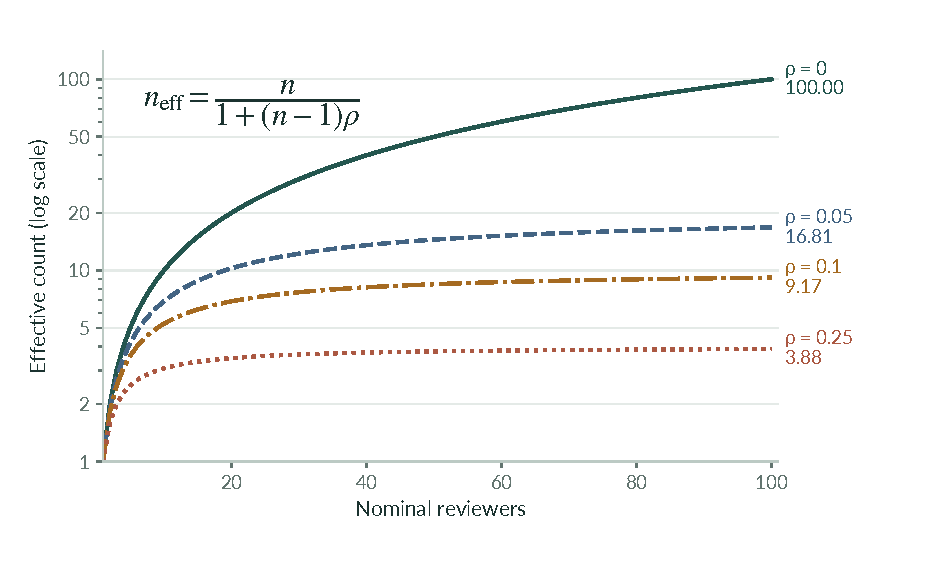
\includegraphics[width=\linewidth]{fig_10_effective_reviewers.pdf}
\caption{Effective reviewer count under the specified equicorrelation model. The logarithmic vertical scale keeps all four curves visible. At $n=100$ and $\rho=0.1$, the effective count is about $9.17$. This formula models variance reduction, not the probability that a mathematical claim is true.}
\label{fig:reviewers}
\end{figure}

For a general positive definite covariance matrix $\Sigma$, consider unbiased linear aggregates $w^\top X$ with $\mathbf 1^\top w=1$.

\begin{theorem}[Minimum-variance covariance-aware weights]
\label{res:17:2}
The unique minimum-variance unbiased linear aggregate has weights
\[
w^*
=
\frac{\Sigma^{-1}\mathbf 1}
{\mathbf 1^\top\Sigma^{-1}\mathbf 1}.
\]
Its variance is
\[
\frac{1}{\mathbf 1^\top\Sigma^{-1}\mathbf 1}.
\]
\end{theorem}

\begin{proof}
Minimize $w^\top\Sigma w$ subject to $\mathbf 1^\top w=1$. The Lagrangian is
\[
L(w,\lambda)=w^\top\Sigma w-2\lambda(\mathbf 1^\top w-1).
\]
Stationarity gives $\Sigma w=\lambda\mathbf 1$, hence $w=\lambda\Sigma^{-1}\mathbf 1$. The constraint gives
\[
\lambda=(\mathbf 1^\top\Sigma^{-1}\mathbf 1)^{-1}.
\]
Positive definiteness makes the objective strictly convex, so the solution is unique. Substitution gives the variance formula.
\end{proof}

\begin{warning}[Bias is not covariance]
\label{res:17:3}
Covariance-aware weighting does not remove a common bias that is absent from the covariance model. If every reviewer shares bias $b$, the mean squared error contains the irreducible term $b^2$.
\end{warning}

Under the model, dependence rather than nominal count determines the variance reduction. Whether a particular review process has this covariance structure is an empirical question. The formula alone neither endorses nor discredits a community judgment.


\section{Shared interpretation, review dependence, and identification}
\label{sec:old25}
\label{sec:interpretation}

The distinction between proof and proof field also matters when many people assess the same mathematics. An individual can evaluate a theorem through the notation, examples, expectations, and disciplinary assumptions available to them. Different reviewers may share these influences. Agreement therefore need not provide independent evidence, although substantive criticism can still identify a real defect. The mathematical contribution of a model lies in making its assumptions explicit, not in diagnosing the motives of reviewers.

\subsection{Correlated noise and persistent common bias}

The covariance model of Section~\ref{sec:correlated-review} measures how dependence reduces the effective information in repeated estimates. It cannot remove a common offset. The next proposition puts both effects into one equation.

\begin{proposition}[MSE with a shared interpretive offset]
\label{res:25:1}
Suppose reviewers report $J_i=\theta+b+\varepsilon_i$, where $\theta$ is the target quantity, $b$ is a fixed shared offset, $\mathbb E\varepsilon_i=0$, $\operatorname{Var}(\varepsilon_i)=\sigma^2$, and $\operatorname{Cov}(\varepsilon_i,\varepsilon_j)=\rho\sigma^2$ for $i\ne j$. For admissible $\rho$, the mean squared error of the reviewer average is
\[
\boxed{\mathbb E(\overline J_n-\theta)^2=b^2+\sigma^2\left(\rho+\frac{1-\rho}{n}\right).}
\]
For fixed $\rho\ge0$, it approaches $b^2+\rho\sigma^2$ as $n\to\infty$.
\end{proposition}
\begin{proof}
The estimation error is $\overline J_n-\theta=b+\overline\varepsilon_n$. Its mean is $b$, and its variance is $\sigma^2\big((1-\rho)/n+\rho\big)$ by summing all diagonal and off-diagonal covariance entries. Mean squared error is variance plus squared bias. Taking the limit completes the proof.
\end{proof}

This formula complements, rather than replaces, the effective reviewer count. Adding reviewers may reduce independent error while leaving the common offset untouched. The existing Python routine \path{shared_bias_mse} computes this model and permits an additional declared variance term for a shared random lens. Its input parameters are model choices, not measured facts about a given intellectual community.

\subsection{When an identity effect can actually be measured}

A claim about identity effects needs a design that can distinguish them from other differences. Hold the mathematical content fixed and let $Y_i(1)$ and $Y_i(0)$ be the fixed potential evaluations of reviewer $i$ under two labels. In a finite set of $N$ reviewers, assign exactly $n_1$ to the first label and $n_0=N-n_1$ to the second, uniformly over assignments with those sizes, where $n_0,n_1>0$. Assume each observed response equals the potential response under its assigned label and does not depend on other assignments. Then the difference of the two sample means is unbiased for $N^{-1}\sum_i(Y_i(1)-Y_i(0))$. Indeed, each reviewer has inclusion probability $n_1/N$ in the first mean and $n_0/N$ in the second, so linearity of expectation gives that identity.

This conclusion concerns the assigned reviewers. Generalizing to a broader population requires a sampling model. Missing responses, shared discussion, or changes to the argument itself can invalidate the simple interpretation. None of these comparisons determines whether the proof is correct. Correctness requires its own mathematical audit.

This distinction is central to a proposed application of Proof Path Theory. One may observe that a presentation changes which branches reviewers explore or how they estimate importance. Those differences become evidence of a contextual effect only after alternative explanations have been addressed. A skeptical review can be correct. Agreement can be justified. The mere presence of community influence neither validates nor invalidates a theorem.

The research opportunity is to connect a typed archive of mathematical claims with controlled studies of how proof paths are selected, compressed, and interpreted. A certified proof core would be held fixed while the accompanying discovery field or contextual labels change. The questions are which alternatives readers recognize, which obstructions they find, and how their subsequent mathematical exploration differs. These are empirical targets for future work, not conclusions established by this finite model.

\subsection{Interpretation and mathematical validity}

The ambient field records exploratory trajectories, the realization theory determines whether specified local models assemble, and the review model describes the effect of declared dependence among numerical judgments. They address different questions. Their common archive makes comparison possible without identifying agreement, coherence, and deductive validity.

These constructions do not yield a general solver for mathematical conjectures, a unique numerical measure of mathematical meaning, a canonical global proof field, or an empirical diagnosis of actual mathematical communities. They provide explicit finite questions with checkable answers and identify the conditions needed for stronger generalizations. Most importantly, they preserve the difference between a valid result and the circumstances through which people discover or evaluate it.



\section{Verification bandwidth and audit queues}
\label{sec:old18}

Let $a_t\geq0$ be candidate arrivals during audit cycle $t$, let $s_t\geq0$ be service capacity, and let $B_t\geq0$ be the unresolved backlog. Suppose arrivals in a cycle are available to that cycle's service. The basic deterministic queue is
\[
B_{t+1}=\max\{0,B_t+a_t-s_t\}.
\]

\begin{theorem}[Constant-rate audit regimes]
\label{res:18:1}
\label{thm:audit-rates}
Suppose $a_t\equiv\lambda$ and $s_t\equiv\mu$.
\begin{enumerate}[label=\textup{(\roman*)}]
\item If $\lambda<\mu$, every finite initial backlog reaches zero after finitely many cycles.
\item If $\lambda=\mu$, the backlog remains constant.
\item If $\lambda>\mu$, the backlog grows linearly with slope $\lambda-\mu$.
\end{enumerate}
\end{theorem}

\begin{proof}
Before the truncation at zero, each cycle adds $\lambda-\mu$. When this quantity is negative, the backlog decreases by a fixed amount until it reaches zero. When it is zero, the backlog is unchanged. When it is positive, the truncation is never active after a nonnegative start, and the backlog is $B_0+t(\lambda-\mu)$.
\end{proof}

\begin{figure}[htbp]
\centering
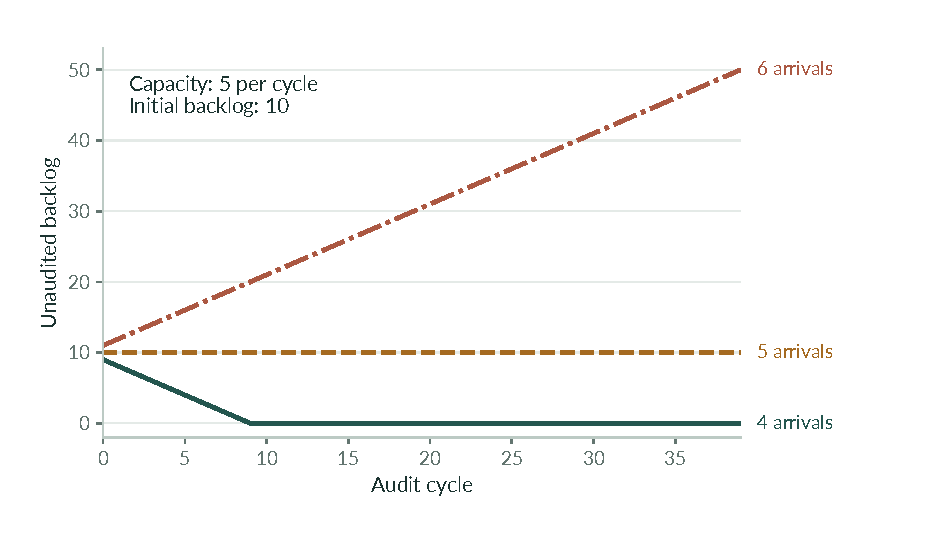
\includegraphics[width=\linewidth]{fig_11_audit_queues.pdf}
\caption{The committed audit example starts with backlog ten and capacity five. Four arrivals per cycle clear the queue, five preserve the backlog, and six increase it. Direct labels replace a separate legend. These are exact trajectories for the declared constant-rate model.}
\label{fig:auditqueue}
\end{figure}

A simple audit priority score is
\[
P(x)
=
\frac{p_{\mathrm{err}}(x)\,c_{\mathrm{consequence}}(x)
\bigl(1+r_{\mathrm{dependency}}(x)\bigr)}
{c_{\mathrm{audit}}(x)}.
\]
Here $p_{\mathrm{err}}(x)\in[0,1]$, the consequence and dependency factors are nonnegative, and $c_{\mathrm{audit}}(x)>0$. Zero-cost checks can be handled separately. This is a declared priority heuristic, not a probability of truth or a proved optimal scheduling rule.


\FloatBarrier
\section{Recursive proof cubes and expansion depth}
\label{sec:old19}

A visible proof step is rarely atomic. A lemma opens into definitions and sublemmas. A computation opens into algorithms, parameters, and exact checks. A citation opens into another dependency graph. Proof Path Theory treats this as recursive refinement.

\begin{definition}[Proof packet and refinement]
\label{res:19:1}
A proof packet is a node presented at one resolution. A refinement replaces that node by a finite subfield whose certified target reconstructs the original node on the declared scope.
\end{definition}

A refinement preserves the certified target on its declared scope. Preservation of other tasks requires a separate recovery condition. Let $R_d:\mathscr A\to\mathcal R_d$ be the representation scheme at depth $d$. A sufficient condition is a map
\[
\pi_d:R_{d+1}(\mathscr A)\longrightarrow R_d(\mathscr A)
\qquad\text{with}\qquad R_d=\pi_d\circ R_{d+1}.
\]
If a task factors as $q=d_q\circ R_d$, then
\[
q=(d_q\circ\pi_d)\circ R_{d+1}.
\]
Hence $R_d\preceq_{\Qcal}R_{d+1}$. Repeated refinements satisfying this condition give the recoverability chain. For a restricted task family, preserving its supported tasks directly can suffice without recovering the entire preceding representation.

A longer derivation is not automatically a richer archive. It may reconstruct the same conclusion while omitting an example, a failed approach, or a provenance record. Those losses must be assessed against the declared task family.

Let $r_d\geq0$ be a declared unresolved-work score and $c_d\geq0$ the cumulative cost. These are model inputs. A small $r_d$ is not, without another theorem, a certificate of a nearly valid proof. The word cube names the layered presentation, not a cubical complex supplied with additional geometric axioms.

\begin{definition}[Goal-relative depth objective]
\label{res:19:2}
For goal $g$ with weights $\alpha_g,\beta_g\ge0$, define
\[
J_g(d)=\alpha_g r_d+\beta_g c_d.
\]
An optimal expansion depth is any minimizer of $J_g$.
\end{definition}

\begin{theorem}[Expansion depth is goal dependent]
\label{res:19:3}
The same proof object can have different optimal expansion depths for different goals.
\end{theorem}

\begin{proof}
Take a proof object with exactly two available depths $d_1<d_2$, with $r_{d_2}<r_{d_1}$ and $c_{d_2}>c_{d_1}$. Direct subtraction shows that $d_2$ is preferred exactly when
\[
\alpha_g(r_{d_1}-r_{d_2})>\beta_g(c_{d_2}-c_{d_1}).
\]
The goal $(\alpha_g,\beta_g)=(1,0)$ strictly prefers $d_2$, whereas $(0,1)$ strictly prefers $d_1$. Since these are the only available depths, each preference is a global optimum. If both weights vanish, every depth is optimal. No division by a possibly zero weight is needed.
\end{proof}

A practical stopping rule selects the first depth satisfying
\[
r_d\le\varepsilon\qquad\text{or}\qquad
\frac{r_{d-1}-r_d}{c_d-c_{d-1}}<\tau.
\]
The first condition uses a declared tolerance. The second applies only at $d\geq1$ with $c_d>c_{d-1}$ and compares the most recent reduction with its extra cost. Zero-cost refinements require separate handling. These stopping rules do not generally minimize $J_g$ over all remaining depths.

Figure~\ref{fig:refinement} and the worked example in Section~\ref{sec:depth-example} give explicit costs and unresolved-work scores for three goals.

Deeper is not automatically better. A formal checker may need primitive steps. A specialist paper may cite a standard theorem. A teaching account may expand only the conceptual bottleneck. An archive may retain a failed branch that neither certificate requires.


\monographpart{Examples, implementation, and boundaries}{Examples and scope}{The final layer is inspectable: source records, computations, certificates, and evidence. Each check has a declared scope, and the open problems remain separate from the implemented finite theory.}

\section{Worked finite examples}
\label{sec:old20}

The accompanying repository contains three canonical JSON proof fields and several auxiliary models. The examples are small enough to inspect by hand and complete enough to exercise the formal distinctions.

\subsection{A fixed AND-DAG}

The field \texttt{examples/and\_dag.json} has required premise $A$, a definition $D$, lemmas $L_1$ and $L_2$, and target $B$. It also contains a worked example, a failed route, and a boundary case. The unique verification core is
\[
\{A,D,L_1,L_2,B\}.
\]
The optional nodes have zero declared verification value for $B$ and positive discovery, meaning, or bridge value. This is the executable instance behind Figure~\ref{fig:loss}.

\subsection{Two certified proofs}

The field \texttt{examples/alternative\_proofs.json} contains a short route and a richer explanatory route. The short route has storage cost $1$, while the richer route has storage cost $3$ and larger meaning and discovery values. Exact certificate search chooses
\[
A\longrightarrow L_{\mathrm{short}}\longrightarrow B
\]
when the objective is storage cost alone. A teaching compiler may rationally choose the other route because it uses a different objective.

\subsection{Set Cover encoded as certificate selection}

The field \texttt{examples/set\_cover\_certificate.json} contains four optional source lemmas and four obligations. Exact search returns the certificate using $S_1$ and $S_3$, with total cost $2$. The particular optimum is not important. The example demonstrates how local alternative derivations create a global combinatorial selection problem.

\subsection{Bridge retention}

The bridge experiment uses ten candidate nodes and sixteen weighted future targets. For budgets zero through five, the script computes both the exact optimum and the greedy solution. The generated data are stored in \texttt{data/retention\_comparison.csv}. On this instance the two curves coincide. The theorem guarantees only the worst-case $(1-1/e)$ factor.

\subsection{Correlated review and audit capacity}

For one hundred equicorrelated reviewers with $\rho=0.1$,
\[
n_{\mathrm{eff}}
=
\frac{100}{1+99(0.1)}
\approx 9.17.
\]
The audit example begins with backlog $10$. Arrivals $4$ and capacity $5$ clear the queue. Equal rates hold the backlog at $10$. Arrivals $6$ and capacity $5$ increase it by one per cycle.

\begin{table}[H]
\centering
\caption{Canonical finite examples and their mathematical roles.}
\begin{tabular}{@{}lll@{}}
\toprule
Object & Computed result & Mathematical role\\
\midrule
AND-DAG & unique five-node core & Theorem~\ref{thm:and-core}\\
Alternative field & minimum cost $1$ & exact finite search\\
Set Cover field & minimum cost $2$ & Theorem~\ref{thm:minimum-certificate} encoding\\
Bridge model & greedy and exact curves & Theorems~\ref{thm:bridge-submodular}--\ref{thm:bridge-greedy}\\
Review model & $n_{\mathrm{eff}}$ formula & Theorem~\ref{thm:review-count}\\
Audit model & three queue regimes & Theorem~\ref{thm:audit-rates}\\
\bottomrule
\end{tabular}
\end{table}


\subsection{An expansion-depth calculation}
\label{sec:depth-example}
For depths $0$ through $6$, take unresolved-work scores
$(1,0.55,0.30,0.18,0.12,0.09,0.075)$ and costs
$(0,0.25,0.65,1.2,2.1,3.5,5.5)$. The declared weights
$(\alpha,\beta)=(1,0.75)$, $(2.5,0.35)$, and $(5,0.15)$ give
minimizing depths $1$, $3$, and $4$, respectively. Their minimum objective
values are $0.7375$, $0.87$, and $0.915$. These follow by evaluating
$\alpha r_d+\beta c_d$ at the seven available depths. The labels certificate,
teaching, and archive name these three supplied objectives rather than
measured preferences of actual readers.

\begin{figure}[htbp]
\centering
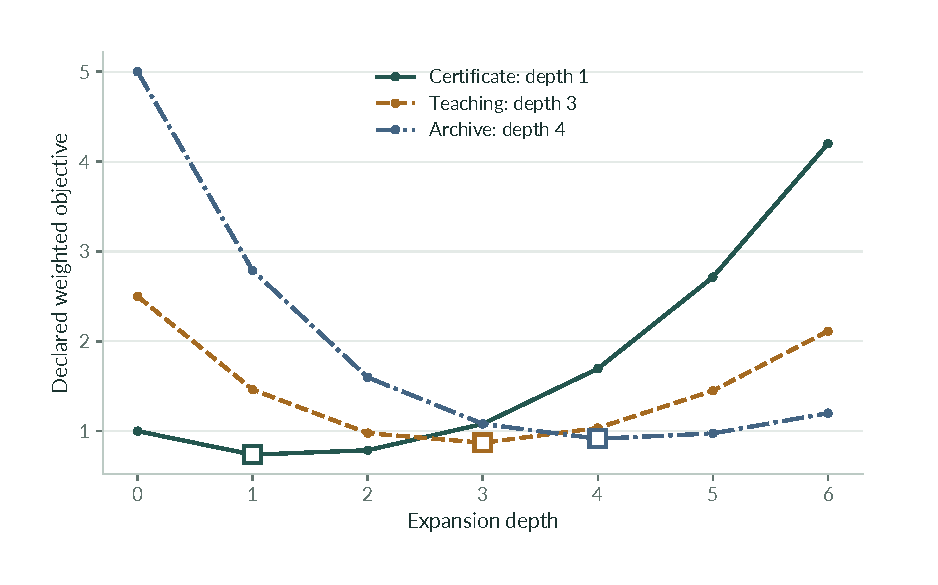
\includegraphics[width=\linewidth]{fig_12_refinement_goals.pdf}
\caption{Three declared objectives on the same finite depth set. Square markers select the exact minimum: depth one for certificate, three for teaching, and four for archive. The weights define these tasks; they are not estimates of how every reader should study a proof.}
\label{fig:refinement}
\end{figure}

\Needspace{12\baselineskip}
\subsection{An independently checkable decoder}

Take two archives with the same certificate output but different retained side answers. The following code executes the collision alternative. It then checks the result without running the producer again.
\begin{lstlisting}[language=Python]
from proof_path_theory import factor_task, verify_factorization
encoding = {"archive0": "certificate", "archive1": "certificate"}
task = {"archive0": "0", "archive1": "1"}
result = factor_task(encoding, task)
assert not result.sufficient
assert verify_factorization(encoding, task, result)
\end{lstlisting}
The witness names both archives. It is evidence that this declared task cannot be recovered from this encoding on this domain. It says nothing about whether the shared proof certificate is valid. The package's new worked script also prints the positive decoder, the protected-rule obstruction, and the semantic-cover derivations.

\section{Reference implementation}
\label{sec:old21}

The repository implements the finite theory as the Python package \texttt{proof\_path\_theory}. The public modules are organized by mathematical responsibility.

\begingroup\small
\begin{longtable}{@{}p{0.24\linewidth}p{0.68\linewidth}@{}}
\toprule
Module & Responsibility\\
\midrule
\endhead
\texttt{model.py} & Typed nodes, justifications, evidence records, acyclicity, ancestry, and finite derivability.\\
\texttt{certificate.py} & Certificate validation, unique AND-DAG cores, exact minimum certificate search, and certificate cost.\\
\texttt{compression.py} & Task sufficiency, recoverability preorder, loss reports, compression debt, representation utilities, and Pareto fronts.\\
\texttt{bridges.py} & Reachability, domination-based criticality, exact retention, greedy retention, and finite submodularity checks.\\
\texttt{review.py} & Equicorrelated covariance, effective reviewer count, generalized least squares, and shared-bias mean squared error.\\
\texttt{audit.py} & Audit queue simulation, rate regimes, and explicit priority scores.\\
\texttt{refinement.py} & Goal-relative refinement decisions, optimal depth, and stopping rules.\\
\texttt{versioning.py} & Affected descendants, append-only checks, ledger snapshots, and provenance digests.\\
\texttt{ambient.py} & Finite declared view fibers, restriction checks, and arrow-cover gluing.\\
\texttt{realization.py} & Exact binary elimination, protected fibers, obstruction witnesses, and observation gain.\\
\texttt{views.py} & Local field models, whole-support gluing, declared countermodels, and intersection diagrams.\\
\texttt{extension.py} & Least models preserving true and false observations, with replayable forbidden-node derivations.\\
\path{semantic_cover.py} & Entailment certificates for redundant supports, countermodels to universal gluing, and checked semantic gluing.\\
\texttt{recovery.py} & Factorization on explicit archive families, collision witnesses, joint task schemes, and decoder composition.\\
\path{trace_codec.py} & Versioned indexed exchange, strict and causal trace replay, and an independent result checker.\\
\texttt{io.py} & Stable JSON import and export for proof fields and certificates.\\
\texttt{cli.py} & Command-line validation, core extraction, minimum certificate search, and certificate audit.\\
\bottomrule
\end{longtable}
\endgroup

\subsection{Command-line interface}

The main commands are:

\begin{lstlisting}[language=bash]
proof-path validate examples/and_dag.json
proof-path core examples/and_dag.json --output core.json
proof-path minimum examples/alternative_proofs.json --output minimum.json
proof-path audit examples/and_dag.json core.json
\end{lstlisting}



\subsection{JSON contract}

A proof field file contains:
\begin{itemize}
\item a schema version and metadata.
\item required premises and targets.
\item typed nodes with value and cost vectors.
\item typed evidence records with scope and certification flags.
\item justifications with premise sets, conclusions, rules, evidence references, and certification flags.
\end{itemize}

The named proof-field schema is intentionally plain. It can be produced by a proof assistant adapter, a research notebook, a theorem ledger, or a hand-written example. The positional trace-exchange format in Section~\ref{sec:trace-wire} is a separate, versioned contract. Neither an imported certification flag nor a successful schema check establishes semantic validity.

\subsection{Tests and build discipline}

The regression suite covers graph validation, derivability, certificate extraction, alternative proofs, schema boundaries, and input validation. It also exercises loss vectors, task sufficiency, bridge coverage, retention, review covariance, audit queues, refinement, version propagation, JSON round trips, and the command line. The dated verification record gives the executed count for each edition.

A separate deterministic cross-check compares the exact certificate solver with brute-force enumeration over eighteen cost profiles, tests the greedy cardinality guarantee on one hundred generated coverage instances, verifies 1,024 retention-algebra identities, and compares the effective-reviewer formula with direct covariance calculations in 114 parameter settings.

The extension cross-check exhausts all forward rule subsets on three ordered nodes, every admitted-leaf set, every positive and negative observation set, and every node-covering patch family. An independent truth-table calculation checks feasibility and universal gluing. A separate enumeration compares encodings, task fibers, joint task partitions, and decoder composition on archive domains of at most four elements. These are bounded finite comparisons, not empirical models of mathematical practice.

The trace conformance suite adds independently enumerated finite models, canonical JSON records, and malformed or altered certificates. Its actual byte stream is processed by the Lean checker built in the current formal run. The report records each verdict and the exact input and output hashes. Rejection of a malformed record is not counted as a proof of an impossible mathematical request.

The general Lean proofs now establish the specified trace checker and typed codec. The Python producer, Python checker implementation, standard text parser, and source-address adapter retain separate conformance evidence.

The tests and cross-checks verify the implementation of finite definitions and examples. They do not replace the proofs in this monograph. Conversely, the proofs do not guarantee that a software implementation is free of defects. The release keeps both forms of verification.


\section{What the theory establishes}
\label{sec:old26}

The finite theory establishes the following structural facts.

\begin{enumerate}
\item A proof field can represent conjunction within a justification and alternatives among justifications without confusing candidate edges with certified edges.
\item Derivability in a finite acyclic selected subfield is well defined and computable in topological order.
\item A fixed AND-DAG, expanded only outside its admitted leaves, has a least certificate pair.
\item Alternative derivations make minimum certificate selection NP-complete in general.
\item Compression is meaningful only relative to a task family.
\item Task-relative recoverability forms a preorder and a quotient partial order.
\item Verification loss, discovery loss, meaning loss, bridge loss, and audit loss can diverge.
\item Expected reconstruction debt decreases monotonically as more required material is retained.
\item Bridge criticality is domination in the declared future-reach graph.
\item Weighted future reach is monotone and submodular.
\item Greedy cardinality retention has the standard $(1-1/e)$ guarantee.
\item Append-only certified updates preserve existing derivability.
\item The forward dependency closure is the least set containing the changed nodes and closed under outgoing dependency edges. It marks potential review, not automatic falsehood.
\item Positive review dependence lowers the variance-equivalent count. Under a positive definite covariance model, generalized least squares gives the minimum-variance unbiased linear aggregate.
\item Constant-rate audit queues have an exact stable, critical, or unstable classification.
\item Optimal proof expansion depth depends on the presentation goal.
\end{enumerate}

These results turn the original methodological insight into a finite mathematical branch with explicit objects, algorithms, complexity, and failure boundaries.

The extension results add three further capabilities. A protected rule-model request returns its least feasible model or a derivation of a forbidden node. A cover has universal gluing exactly when its visible rules entail every original rule. A representation admits a task decoder exactly when equal encodings have equal task answers. These outputs are respectively model witnesses, rule derivations, and decoding or collision witnesses. None can replace the others merely because it is called a certificate.


\noindent The realization theory gives the proof field a contravariant diagram of local models and an explicit equivalence with its coherent sections. Whole-support gluing proves extension from suitably covering patches. The protected linear alternative classifies feasible fibers and supplies normalized witnesses for infeasibility. Exact finite-field counts yield an information formula only after a uniform distribution is chosen. The native exporter supplies syntactic dependencies from compiled declarations, not the complete history of discovery.


\section{Limitations and claim boundaries}
\label{sec:old27}

Proof Path Theory does not establish a theorem by preserving the history of an argument. A richly documented wrong proof remains wrong. Bridge value is not validity. Explanatory power is not validity. Consensus is not validity. The certified subfield remains the object that carries deductive force.

The dependency graph is a declared model. It records the dependencies that were formalized, not every historical influence on discovery. Tacit knowledge, visual intuition, unrecorded conversations, and changes in vocabulary may be absent.

The value and cost coordinates are task models. Verification can often be specified sharply. Meaning and future bridge value are partly prospective. Their use is justified when assumptions are stated, not when the numbers are treated as intrinsic physical constants.

The finite bridge graph does not predict every future theorem. It supports conditional statements of the form: under these declared future targets and transfer edges, this retention policy preserves this amount of modeled reach.

The exact minimum certificate algorithm is exponential in the worst case. The package makes this limitation explicit through a search-state bound.

The review and queue models are deliberately elementary. They isolate dependence and capacity effects, but they do not model every institutional or psychological feature of mathematical review.

Finally, the monograph does not claim that graphs, hypergraphs, proof theory, submodular optimization, covariance-aware aggregation, or queueing recurrences were invented here. The contribution is the formal assembly of these structures around proof compression, discovery fields, mathematical memory, and versioned proof portfolios.


\paragraph{The remaining implementation boundary.} Theorem~\ref{res:trace:json} proves the meaning of an accepted decoded answer. It does not prove that every named-field export preserves its source, or that the text parser and Python producer always realize that contract. Those are the next refinement obligations, not hypotheses silently supplied by successful tests.

\section{Open theorem program}
\label{sec:old28}

The finite protected-extension, semantic-cover, and attained-decoder problems developed in this edition are closed under their stated hypotheses. The questions below concern stronger interfaces. In particular, the rule transport sends one source rule to one target rule and is not asserted to be a general equivalence of proof fields. A transport into a derived target proof, executable correctness of the producers, and richer semantic objects remain distinct next steps.


\begin{problem}[Proof-path view functors and comparison]
\label{res:28:1}
The declared-field local-model functor and whole-support gluing are established here. Extend the checked interface to richer proof-state representations, and verify the implementation of general proof assistant adapters. Determine when objects with symmetry require nonabelian or higher descent rather than the strict set-valued construction.
\end{problem}

\begin{problem}[Counterfactual proof-search observations]
\label{res:28:2}
Study which observations on a finite realization fiber yield the greatest task-relative reduction of uncertainty per unit cost. Extend the binary rank theorem to controlled infinite or nonlinear settings only after specifying distributions, admissible questions, and the semantics of proof state.
\end{problem}

\begin{problem}[Collective evaluation without shared-context confounding]
\label{res:28:3}
Design preregistered evaluations of identical certified mathematics under randomized labels and alternative explanatory contexts. Separate measurement of interpretation differences from independent verification of correctness, and test whether models of correlated review predict actual audit errors.
\end{problem}



Further directions include the following problems.

\begin{problem}[Infinite proof fields]
\label{res:28:4}
Develop locally finite and countable proof fields with conditions guaranteeing that finite certificates approximate an infinite derivation without losing domain or convergence information.
\end{problem}

\begin{problem}[Parameterized certificate complexity]
\label{res:28:5}
Classify minimum certificate selection by treewidth, number of alternative justifications, justification arity, shared-subproof width, and target count. Identify fixed-parameter tractable regimes and approximation bounds.
\end{problem}

\begin{problem}[Probabilistic bridge calibration]
\label{res:28:6}
Replace declared bridge weights by calibrated posterior models while keeping conjectural reach separate from certified derivability.
\end{problem}

\begin{problem}[Proof assistant interoperability]
\label{res:28:7}
Construct adapters that export stable claim identifiers, primitive dependencies, scopes, and proof terms from existing formal systems into the common proof-field schema.
\end{problem}

\begin{problem}[Higher proof transformations]
\label{res:28:8}
Model transformations between proofs, transformations between transformations, and coherent compiler pipelines in a higher categorical setting.
\end{problem}

\begin{problem}[Privacy and attribution]
\label{res:28:9}
Design proof archives that preserve provenance and priority while allowing private notes, embargoed routes, and sensitive collaboration records to remain access controlled.
\end{problem}

\begin{problem}[Empirical validation]
\label{res:28:10}
Study real mathematical projects to estimate recovery costs, audit bottlenecks, and the predictive value of bridge-retention scores. Such work should test the models rather than assume them.
\end{problem}

\begin{problem}[Distributed audit systems]
\label{res:28:11}
Extend the queue model to heterogeneous reviewers, dependent tasks, rework, priority classes, and claims whose audit cost changes after neighboring claims are resolved.
\end{problem}


\clearpage
\section{Conclusion}
\label{sec:old29}

A proof certificate and its surrounding proof field answer different mathematical questions. The field need not consist only of viable derivations. It can retain failed strategies and genuine local refutations without allowing either to masquerade as global unprovability. A checked contravariant system of local field models gives an explicit bridge to Komorebi Space. Whole-support coverage identifies a constraint that pairwise dependencies can miss. The semantic-cover criterion now determines exactly when visible rules recover a missing constraint. In the linear finite case, protected observations admit exact success or failure certificates and a measurable information gain. A separate review model distinguishes proof correctness from correlated social interpretation.



A final proof is indispensable, but it is not always the whole mathematical object. The theory distinguishes the certificate from the declared field in which it is recorded. It gives that field typed nodes, alternative justifications, evidence records, task-relative compressions, bridge graphs, version histories, and explicit audit models.

The central distinction is between derivability within a declared inference system and the wider information retained by its archive. Certified closure records which claims follow from admitted leaves and accepted rules. Its interpretation as mathematical validity depends on the soundness of those leaves and rules. Discovery information serves different tasks: explaining a definition, locating a failed method, preserving a comparison, or opening a route to another problem.

Compression can preserve the present derivation while losing those other capabilities. Proof Path Theory makes that difference explicit through task families, recovery maps, extension problems, and versioned evidence. The certificate and the surrounding field should therefore be maintained together, with their logical roles kept distinct.

The final thesis is therefore:
\[
\boxed{\begin{minipage}{0.88\linewidth}
A proof should be published as a certificate and maintained as a versioned proof field. The certificate preserves deductive validity. The larger field preserves the dependencies, alternatives, examples, failures, provenance, and bridges from which later mathematics may grow.
\end{minipage}}
\]


\FloatBarrier
\clearpage
\appendix
\markboth{Reference material}{Reference material}
\section{Notation and hypotheses}
\label{app:notation}

Letters are local to a section. In particular, $A$ denotes required premises in a proof field, but a matrix in the binary examples. The type declarations, not the letter alone, determine the object.

\begingroup\small
\begin{longtable}{@{}L{0.24\linewidth}L{0.71\linewidth}@{}}
\toprule
Symbol & Meaning \\
\midrule
\endhead
$\Pcal$, $V$, $\Jcal$ & A declared proof field, its nodes, and its justifications. \\
$A$, $L$, $T_0$ & Required premises, admissible leaves, and requested targets, with $A\subseteq L$. \\
$(K,H)$ & Selected nodes and certified justification records. Only usable rules contribute to derivability. \\
$D_{\mathrm{cert}}(K,H)$ & The least certified closure in the selected record. \\
$\Anc_L(T_0)$ & Backward ancestry expanded only outside the admissible leaves. \\
$\mathcal M_F(U)$ & Local models on patch $U$ satisfying all certified rules supported entirely in $U$. \\
$\Gamma(\mathcal M_F)$ & Coherent families of those local models under restriction. \\
$\operatorname{cl}_F(S)$ & The least declared rule model containing the positive observations $S$ and all admitted leaves. \\
$\operatorname{Ext}_F(S,N)$ & Rule models containing $S$ and avoiding the negative observations $N$. \\
$F_{\mathcal U}$ & The same field with only rules whose entire supports appear in a covering patch. \\
$Q(a)=(q_i(a))_i$ & The joint task representation, least in retained distinctions for its task family. \\
$\mathscr A$, $C$, $q$ & A class of possible archives, an encoding scheme, and a task on that class. \\
$P_K(S)=S\cap K$ & Pure retention of records selected by a fixed mask. \\
$D:E\to R$, $p:E\to S$ & A linear defect and a protected observable. The repair condition is $Dy=0$, $p(y)=p(x)$. \\
$H=\ker D\cap\ker p$ & The ambiguity space of a nonempty protected fiber. This $H$ is not a set of justifications. \\
$U_M(S)$ & Weighted target reach from the mandatory starts and a selected supplement, in a fixed directed bridge graph. \\
$n_{\mathrm{eff}}$ & A real, variance-equivalent review count in the specified covariance model. \\
\bottomrule
\end{longtable}
\endgroup

\subsection*{Assumptions that change the conclusions}
The unique-core theorem uses backward expansion that stops at admissible leaves and proves a least \emph{pair} of record sets. The compression results quantify over a whole archive class with one decoder for each task. Weighted domination counts only targets reachable before deletion. The greedy ratio requires a positive cardinality budget, with zero and saturated budgets handled separately.

Whole-support gluing is sufficient when the patches cover all nodes and every complete certified rule support. More generally, node coverage and entailment of every original rule by the visible rules are necessary and sufficient for universal gluing. Merely covering pairwise dependencies is not sufficient in general. The linear alternative requires a field. General algebraic functionals need not be bounded under an added topology. The information formula requires a finite field, a finite-dimensional feasible affine fiber, and a uniform distribution.

Endpoint equivalence fixes the complete assumption context. A refinement chain preserves the chosen tasks only when the corresponding recovery condition holds. The unrestricted positive-rule model always contains the full node set as a model. Nonempty global model spaces can still have empty prescribed extension fibers. Provenance change detection distinguishes information lost during serialization from collisions of different serialized bytes.

The review mean is unbiased only when its error means vanish. Its effective count requires positive marginal variance and positive variance of the mean. A minimum-variance aggregate allows real weights and assumes a known positive definite covariance matrix. No probability of mathematical correctness follows from these assumptions alone.



\clearpage
\section{Theorem ledger}
\label{app:ledger}

\emph{Written} denotes a written proof. \emph{Lean} denotes the specified interface with fresh compiler and kernel-replay evidence in this edition, not a formalization of the entire monograph. \emph{Mixed} distinguishes checked counts from their written probabilistic interpretation. The separate Lean concordance lists every source declaration and its scope.

\begingroup\small
\renewcommand{\arraystretch}{1.04}
\begin{longtable}{@{}L{0.115\linewidth}L{0.70\linewidth}L{0.105\linewidth}@{}}
\toprule
{\sffamily\small ID} & {\sffamily\small RESULT AND IMPLEMENTATION SUPPORT} & {\sffamily\small EVIDENCE}\\
\midrule
\endfirsthead
\toprule
{\sffamily\small ID} & {\sffamily\small RESULT AND IMPLEMENTATION SUPPORT} & {\sffamily\small EVIDENCE}\\
\midrule
\endhead
\bottomrule
\endfoot
PPT-001 & Finite derivability is unique and computable in topological order.\newline{\footnotesize\color{KomorebiMuted}\path{ProofField.derive}} & {\sffamily\small\color{KomorebiTeal}Written}\\[0pt]
PPT-002 & An AND-DAG has a least certificate pair, stopping at admissible leaves.\newline{\footnotesize\color{KomorebiMuted}\path{unique_and_dag_certificate}} & {\sffamily\small\color{KomorebiTeal}Written}\\[0pt]
PPT-003 & AND-DAG core extraction is linear with indexed adjacency.\newline{\footnotesize\color{KomorebiMuted}graph algorithm, not a runtime certificate} & {\sffamily\small\color{KomorebiTeal}Written}\\[0pt]
PPT-004 & Minimum Certificate Decision is NP-complete.\newline{\footnotesize\color{KomorebiMuted}Set Cover example} & {\sffamily\small\color{KomorebiTeal}Written}\\[0pt]
PPT-005 & Certified paths transport functorially.\newline{\footnotesize\color{KomorebiMuted}structural theorem} & {\sffamily\small\color{KomorebiTeal}Written}\\[0pt]
PPT-006 & Local auditable certificates compose under a certificate functor.\newline{\footnotesize\color{KomorebiMuted}structural theorem} & {\sffamily\small\color{KomorebiTeal}Written}\\[0pt]
PPT-007 & Task information loss follows from compression collisions.\newline{\footnotesize\color{KomorebiMuted}task API} & {\sffamily\small\color{KomorebiTeal}Lean}\\[0pt]
PPT-008 & Recoverability is a preorder.\newline{\footnotesize\color{KomorebiMuted}\path{recoverability_preorder}} & {\sffamily\small\color{KomorebiTeal}Written}\\[0pt]
PPT-009 & The quotient by mutual recoverability is a partial order.\newline{\footnotesize\color{KomorebiMuted}equivalence API} & {\sffamily\small\color{KomorebiTeal}Written}\\[0pt]
PPT-010 & Least sufficient retention masks depend on the task family.\newline{\footnotesize\color{KomorebiMuted}finite countermodel} & {\sffamily\small\color{KomorebiTeal}Written}\\[0pt]
PPT-011 & Zero verification loss can coexist with positive discovery loss.\newline{\footnotesize\color{KomorebiMuted}AND-DAG example} & {\sffamily\small\color{KomorebiTeal}Written}\\[0pt]
PPT-012 & Compression debt is monotone under retention.\newline{\footnotesize\color{KomorebiMuted}\path{compression_debt}} & {\sffamily\small\color{KomorebiTeal}Written}\\[0pt]
PPT-013 & Bridge criticality equals target domination.\newline{\footnotesize\color{KomorebiMuted}\path{dominated_targets}} & {\sffamily\small\color{KomorebiTeal}Written}\\[0pt]
PPT-014 & Weighted future reach is monotone and submodular.\newline{\footnotesize\color{KomorebiMuted}exhaustive finite checker} & {\sffamily\small\color{KomorebiTeal}Written}\\[0pt]
PPT-015 & Greedy cardinality retention achieves at least $1-1/e$ for positive feasible cardinality budgets.\newline{\footnotesize\color{KomorebiMuted}greedy and exact solvers} & {\sffamily\small\color{KomorebiTeal}Written}\\[0pt]
PPT-016 & Append-only certified updates preserve derivability.\newline{\footnotesize\color{KomorebiMuted}versioning check} & {\sffamily\small\color{KomorebiTeal}Written}\\[0pt]
\pagebreak
PPT-017 & Forward dependency closure is the minimal closed syntactic review set.\newline{\footnotesize\color{KomorebiMuted}\path{affected_descendants}} & {\sffamily\small\color{KomorebiTeal}Written}\\[0pt]
PPT-018 & Equicorrelated review has the stated effective count.\newline{\footnotesize\color{KomorebiMuted}covariance implementation} & {\sffamily\small\color{KomorebiTeal}Written}\\[0pt]
PPT-019 & GLS weights minimize unbiased linear review variance.\newline{\footnotesize\color{KomorebiMuted}\path{generalized_least_squares_weights}} & {\sffamily\small\color{KomorebiTeal}Written}\\[0pt]
PPT-020 & Constant-rate audit queues have exact stable, critical, and unstable regimes.\newline{\footnotesize\color{KomorebiMuted}queue simulation} & {\sffamily\small\color{KomorebiTeal}Written}\\[0pt]
PPT-021 & Optimal expansion depth depends on the goal.\newline{\footnotesize\color{KomorebiMuted}refinement implementation} & {\sffamily\small\color{KomorebiTeal}Written}\\[0pt]
PPT-022 & Pure retention projections commute and are idempotent.\newline{\footnotesize\color{KomorebiMuted}\path{retention_projection}} & {\sffamily\small\color{KomorebiTeal}Written}\\[0pt]
PPT-023 & Retention masks form a Boolean lattice.\newline{\footnotesize\color{KomorebiMuted}\path{retention_meet}, \path{retention_join}} & {\sffamily\small\color{KomorebiTeal}Written}\\[0pt]
PPT-024 & A locally refuted route can coexist with another certified route.\newline{\footnotesize\color{KomorebiMuted}Alternative justification field} & {\sffamily\small\color{KomorebiTeal}Written}\\[0pt]
PPT-025 & A checked local refutation persists under unchanged interpretation.\newline{\footnotesize\color{KomorebiMuted}Scoped witness principle} & {\sffamily\small\color{KomorebiTeal}Written}\\[0pt]
PPT-026 & Finite arrow-covered matching views glue uniquely.\newline{\footnotesize\color{KomorebiMuted}\path{FiniteViewSystem.glue}} & {\sffamily\small\color{KomorebiTeal}Lean}\\[0pt]
PPT-027 & Protected realizations admit exact solutions or obstruction witnesses, with classified fibers.\newline{\footnotesize\color{KomorebiMuted}\path{analyze_affine_realizations}} & {\sffamily\small\color{KomorebiTeal}Lean}\\[0pt]
PPT-028 & Finite affine fibers have exact observation counts. Uniform entropy is a written corollary.\newline{\footnotesize\color{KomorebiMuted}Lean counts and binary tests} & {\sffamily\small\color{KomorebiTeal}Mixed}\\[0pt]
PPT-029 & Common offset and correlated error have the displayed reviewer MSE.\newline{\footnotesize\color{KomorebiMuted}\path{shared_bias_mse}} & {\sffamily\small\color{KomorebiTeal}Written}\\[0pt]
PPT-030 & Declared derivability equals membership in every declared field model.\newline{\footnotesize\color{KomorebiMuted}Closure and countermodels} & {\sffamily\small\color{KomorebiTeal}Lean}\\[0pt]
PPT-031 & Local models form a contravariant diagram with an explicit realization equivalence.\newline{\footnotesize\color{KomorebiMuted}\path{Field.modelEquivSections}} & {\sffamily\small\color{KomorebiTeal}Lean}\\[0pt]
PPT-032 & Whole-support matching local models glue. Pairwise coverage can fail.\newline{\footnotesize\color{KomorebiMuted}Proof-field views and counterexample} & {\sffamily\small\color{KomorebiTeal}Lean}\\[0pt]
\pagebreak
PPT-033 & All predicate tasks are sufficient exactly for injective encodings.\newline{\footnotesize\color{KomorebiMuted}Compression collision theorem} & {\sffamily\small\color{KomorebiTeal}Lean}\\[0pt]
PPT-034 & Attained decoding is equivalent to fiber constancy. The decoder is unique on attained values.\newline{\footnotesize\color{KomorebiMuted}Recovery and finite decoder checks} & {\sffamily\small\color{KomorebiTeal}Lean}\\[0pt]
PPT-035 & Joint tasks are sufficient exactly when each coordinate task is. Recovery maps compose.\newline{\footnotesize\color{KomorebiMuted}Recovery and joint partitions} & {\sffamily\small\color{KomorebiTeal}Lean}\\[0pt]
PPT-036 & Protected rule data have an extension exactly when their least closure avoids the forbidden nodes.\newline{\footnotesize\color{KomorebiMuted}Extension and independent trace replay} & {\sffamily\small\color{KomorebiTeal}Lean}\\[0pt]
PPT-037 & Closing earlier data before later data preserves the closure. Adding observations preserves obstructions.\newline{\footnotesize\color{KomorebiMuted}Extension} & {\sffamily\small\color{KomorebiTeal}Lean}\\[0pt]
PPT-038 & A cover has universal gluing exactly when its visible rules entail every original rule.\newline{\footnotesize\color{KomorebiMuted}SemanticCover and finite cover certificates} & {\sffamily\small\color{KomorebiTeal}Lean}\\[0pt]
PPT-039 & Typed rule transports preserve derivations, pull models back, and transport obstruction witnesses.\newline{\footnotesize\color{KomorebiMuted}RuleTransport} & {\sffamily\small\color{KomorebiTeal}Lean}\\[0pt]
PPT-040 & A valid rule transport can collapse compatible source observations into an impossible target request.\newline{\footnotesize\color{KomorebiMuted}ExtensionExamples} & {\sffamily\small\color{KomorebiTeal}Lean}\\[0pt]
PPT-041 & Hashing cannot add recoverable tasks. Restricted injectivity prevents further task loss.\newline{\footnotesize\color{KomorebiMuted}Recovery} & {\sffamily\small\color{KomorebiTeal}Lean}\\[0pt]
PPT-042 & Executable trace replay preserves derivability and composes.\newline{\footnotesize\color{KomorebiMuted}Trace and TraceCompleteness} & {\sffamily\small\color{KomorebiTeal}Lean}\\[0pt]
PPT-043 & Accepted complete traces identify the least seeded model.\newline{\footnotesize\color{KomorebiMuted}Trace and TraceCompleteness} & {\sffamily\small\color{KomorebiTeal}Lean}\\[0pt]
PPT-044 & Accepted forbidden-node witnesses exist exactly for infeasible protected requests.\newline{\footnotesize\color{KomorebiMuted}Trace and TraceCompleteness} & {\sffamily\small\color{KomorebiTeal}Lean}\\[0pt]
PPT-045 & Typed JSON encoding has a left inverse and is injective.\newline{\footnotesize\color{KomorebiMuted}Trace.Wire} & {\sffamily\small\color{KomorebiTeal}Lean}\\[0pt]
PPT-046 & Accepted JSON records certify the exact decoded protected answer.\newline{\footnotesize\color{KomorebiMuted}Trace.Wire} & {\sffamily\small\color{KomorebiTeal}Lean}\\[0pt]
PPT-047 & Valid indexed problems derive only bounded node addresses.\newline{\footnotesize\color{KomorebiMuted}Trace.Wire} & {\sffamily\small\color{KomorebiTeal}Lean}\\[0pt]
\end{longtable}
\renewcommand{\arraystretch}{1.0}
\endgroup

\clearpage
\section{Reproduction and verification records}
\label{app:reproduction}

The package includes written proofs, exact finite producers and independent result checkers, and a fresh pinned Lean run. All eighteen modules were rebuilt and replayed. The mathematical imports remain cached and are not represented as freshly rebuilt dependencies. The current compiler record is \path{evidence/formal_1.8.0/}, while older evidence retains its original version. Source changes and the new mathematical environments are listed in the current progress ledger and publication report.

Before modifying the extracted package, check the delivered files:
\begin{lstlisting}[language=bash]
python scripts/check_manifest.py
\end{lstlisting}
Then run the finite and publication checks:
\begin{lstlisting}[language=bash]
python -m pip install -e ".[release]" --no-build-isolation
python -m pytest -o addopts='' -q
python scripts/deep_validation.py
python scripts/verify_bridge.py
python scripts/check_recovery_extension.py
python scripts/check_trace_exchange.py
python scripts/verify_publication_edition.py
\end{lstlisting}

Regenerate the exact figures with:
\begin{lstlisting}[language=bash]
python scripts/design_figures.py
\end{lstlisting}
The publication edition is 1.8.0 and the Python distribution is 1.6.0. This distribution adds a versioned trace-exchange codec, an independent indexed checker, and export/check commands without changing the existing named-field schema or provenance byte format. Its historical migration remains documented in \path{docs/PROVENANCE_FORMAT.md}. Installation may obtain build and numerical dependencies unless they are already supplied locally.

The manuscript can be rebuilt independently from \path{docs/}:
\begin{lstlisting}[language=bash]
cd docs
pdflatex -interaction=nonstopmode -halt-on-error Proof_Path_Theory.tex
pdflatex -interaction=nonstopmode -halt-on-error Proof_Path_Theory.tex
pdflatex -interaction=nonstopmode -halt-on-error Proof_Path_Theory.tex
\end{lstlisting}

\clearpage
\subsection*{Formal and cross-language replay}
A separate formal replay, with the pinned runtime already available, uses:
\begin{lstlisting}[language=bash]
python scripts/verify_lean.py --runtime /path/to/portable-kit
\end{lstlisting}

For PowerShell, extraction precedes installation:
\begin{lstlisting}[language={},basicstyle=\ttfamily\fontsize{9.5}{11.4}\selectfont]
$zip = '.\Proof_Path_Theory_Monograph_1.8.0.zip'
Expand-Archive -LiteralPath $zip -DestinationPath '.\proof-path-release'
Set-Location '.\proof-path-release\Proof_Path_Theory_Monograph_v1.8.0'
python scripts/check_manifest.py
python -m pip install -e ".[release]" --no-build-isolation
python -m pytest -o addopts='' -q
\end{lstlisting}

The trace interface can be exercised without a Lean runtime:
\begin{lstlisting}[language=bash]
proof-path wire-export examples/and_dag.json --negative B --output-prefix trial
proof-path wire-check trial.problem.json trial.certificate.json
\end{lstlisting}
The export writes the fixed indexed problem, the checked result, and the node/rule address book separately. The general AST theorem is in \path{ProofPath.TraceWire}. The executed byte adapter is \path{formal/CheckTraceJson.lean}; the fresh formal verifier runs it against the generated canonical exchange cases. The address book must still be checked against the intended source snapshot.

The dated report identifies the commands actually run. These checks do not supply independent peer review, universal software verification, or empirical validation of the social models. The redistribution-license decision remains open.

\clearpage
\section{A complete minimal proof-field record}
\label{app:schema}

The following record defines both its premise and its target. It is a complete importable example rather than a schema fragment with an unresolved target reference. The rule is explicitly assumed for this demonstration. Its declared certification must not be mistaken for a proof of an arbitrary implication between the displayed labels.

\begin{lstlisting}[language={},basicstyle=\ttfamily\fontsize{9.5}{11.4}\selectfont]
{
  "schema_version": "1.0",
  "premises": ["A"],
  "targets": ["B"],
  "nodes": [
    {"id": "A", "label": "Premise A", "kind": "premise"},
    {"id": "B", "label": "Target B", "kind": "claim"}
  ],
  "evidence": [
    {
      "id": "e-rule",
      "kind": "assumption",
      "source": "Declared demonstration rule A implies B",
      "scope": "This finite inference model only",
      "certifies": true
    }
  ],
  "justifications": [
    {
      "id": "j1",
      "premises": ["A"],
      "conclusion": "B",
      "rule": "assumed implication",
      "certified": true,
      "evidence_ids": ["e-rule"]
    }
  ]
}
\end{lstlisting}

The file \path{examples/minimal_monograph.json} contains this record. The public importer checks its identifiers and Boolean fields, and declared closure reaches \texttt{B}. Mathematical soundness still requires the explicit interpretation contract of Section~\ref{sec:old24}.

\clearpage
\phantomsection
\addcontentsline{toc}{section}{References}
\begin{thebibliography}{99}

\bibitem{komorebi-space}
Komorebi P.
\textit{Komorebi Space: Coherent Realizations, Obstructions, and Descent}.
Monograph, 2026. The finite proof-field view construction here is a relative application of its strict coherent realization principle, not a claim of unrestricted semantic completeness.

\bibitem{buss}
S. R. Buss, editor.
\textit{Handbook of Proof Theory}.
Elsevier, 1998.

\bibitem{cover-thomas}
T. M. Cover and J. A. Thomas.
\textit{Elements of Information Theory}.
Second edition, Wiley, 2006.

\bibitem{diestel}
R. Diestel.
\textit{Graph Theory}.
Fifth edition, Springer, 2017.

\bibitem{garey-johnson}
M. R. Garey and D. S. Johnson.
\textit{Computers and Intractability: A Guide to the Theory of NP-Completeness}.
W. H. Freeman, 1979.

\bibitem{knuth}
D. E. Knuth.
\textit{Literate Programming}.
CSLI Publications, 1992.

\bibitem{maclane}
S. Mac Lane.
\textit{Categories for the Working Mathematician}.
Second edition, Springer, 1998.

\bibitem{nemhauser}
G. L. Nemhauser, L. A. Wolsey, and M. L. Fisher.
An analysis of approximations for maximizing submodular set functions I.
\textit{Mathematical Programming}, 14:265--294, 1978.

\bibitem{troelstra}
A. S. Troelstra and H. Schwichtenberg.
\textit{Basic Proof Theory}.
Second edition, Cambridge University Press, 2000.

\end{thebibliography}

\end{document}
